%el partie elli men mellouel thot feha le type de document exple article.....
%ahna bech na3mlou rapport pfe donc nektbou report
%12pt: taille de police (recommandé)
%a4paper: type de papier
\documentclass[12pt,a4paper]{report}

%entre \begin[document] et \end{document} est le contenu principale de la page
%======creer preambule=====
%les packages 
%1. traitement des caractères spéciaux(affichage correcte)
\usepackage[T1]{fontenc}
\usepackage[utf8]{inputenc}
\usepackage{subcaption}
\setcounter{secnumdepth}{3}
  
 \usepackage[french]{minitoc} %2. yokhrejli mini sommaire mta3 kol chapitre
%\etocsetnexttocdepth{subsection} %list subsections
\usepackage[top=2.5cm, bottom=2.5cm, left=2.5cm, right=2.5cm]{geometry}% geometry package des marges des pages, (tnajem matektebech[] w howa yhotlek les tailles par defaut 
\usepackage[pdftex]{graphicx} %package des images, option pdftex spécifier que le document sera compilé avec pdfLaTeX
\usepackage[colorlinks=true, linkcolor=black]{hyperref} %for creating links in the pdf version and other additional pdf attributes, no effect on the printed document
\usepackage[final]{pdfpages} %est utilisée pour inclure des pages PDF externes dans votre document LaTeX.final les documents ne sont pas cliquable(exple page de garde)
\usepackage{float} %pour bien positionner les figures(pour forcer a positionner les figures fl blasa elli ena nheb aleha)
\usepackage{pslatex} % for times new roman,
\usepackage{url} %pour les liens url
\usepackage{adjustbox} %pour ajuster la taille des tableaux et des figures
\usepackage{array} %  pour créer et personnaliser des tableaux dans votre document
\usepackage{setspace} %pour controler l'espace entre les lignes \onehalfspacing \singlespacing \doublespacing
\usepackage{enumerate}%listes à numéros
\usepackage{longtable}%tableaux sur plusieurs pages(des tableaux twel yet9assmou ala des pages)
\usepackage{multirow}% fusion 2 lignes ou 2 colonnes dans un tableau
\usepackage{enumitem}%pour des items star fleche etc(tekhtar kifech tr9em el liste - .*....)
\usepackage{tabularx}
\usepackage{booktabs} % Pour les règles professionnelles (\toprule, \midrule, \bottomrule)
\usepackage{array}    % Pour mieux contrôler les colonnes
\usepackage[table]{xcolor} % Pour les couleurs de fond
\usepackage[french]{babel}
\usepackage[font=small,labelfont=bf]{caption}%les caption seront en taille small et gras(figure1, table1) (kol tableau andou titre
\onehalfspacing % basic elli dima nestamlou , teb3a el package setspace

% Définir la longueur de l'espacement entre les paragraphes
\setlength{\parskip}{10pt} % Réglez la valeur selon vos préférences(9adeh el espaces bin les paragraphes)
%-------------------
%pour choisir un style pour les chapitres
%https://latex-tutorial.com/fancy-chapters-latex/
\usepackage[Glenn]{fncychap}
%\usepackage[Conny]{fncychap}
%\usepackage[Bjarne]{fncychap}

% ======Configuration des en-têtes et des pieds de page
\usepackage{fancyhdr}
\pagestyle{fancy}
\fancyhf{}

%\fancyhead[R]{\rightmark} %pour les sections en haut de l'ntête
%bech trigel el entête mtae3ek
\fancyhead[LE,RO]{\nouppercase{\leftmark}}  % Chapter name in the outer side of even and odd pages
%lorsque vous utilisez \leftmark dans l'en-tête, LaTeX récupère automatiquement le nom du chapitre en cours. De même, lorsque vous utilisez \rightmark, LaTeX récupère le nom de la section en cours. 
\fancyfoot[LE,RO]{\thepage} % Page number in the outer side of even and odd pages

\renewcommand{\headrulewidth}{0.4pt} % Thickness of the header rule line
\renewcommand{\footrulewidth}{0.4pt} % No footer rule line

\makeatletter
\renewcommand{\numberline}[1]{%
  \settowidth\@tempdimb{#1}%
  \ifdim\@tempdima<\@tempdimb
    \hb@xt@\@tempdimb{#1\hfil}\hspace{0.5em}%
  \else
    \hb@xt@\@tempdima{#1\hfil}%
  \fi
}
\makeatother
\usepackage{chngcntr}
\counterwithin{figure}{chapter}
%=============document principal ========
\begin{document}
\cleardoublepage % Pour commencer une nouvelle page  si nécessaire
%======pour mettre la page de garde il faut: enlever le commentaire ci dessous====
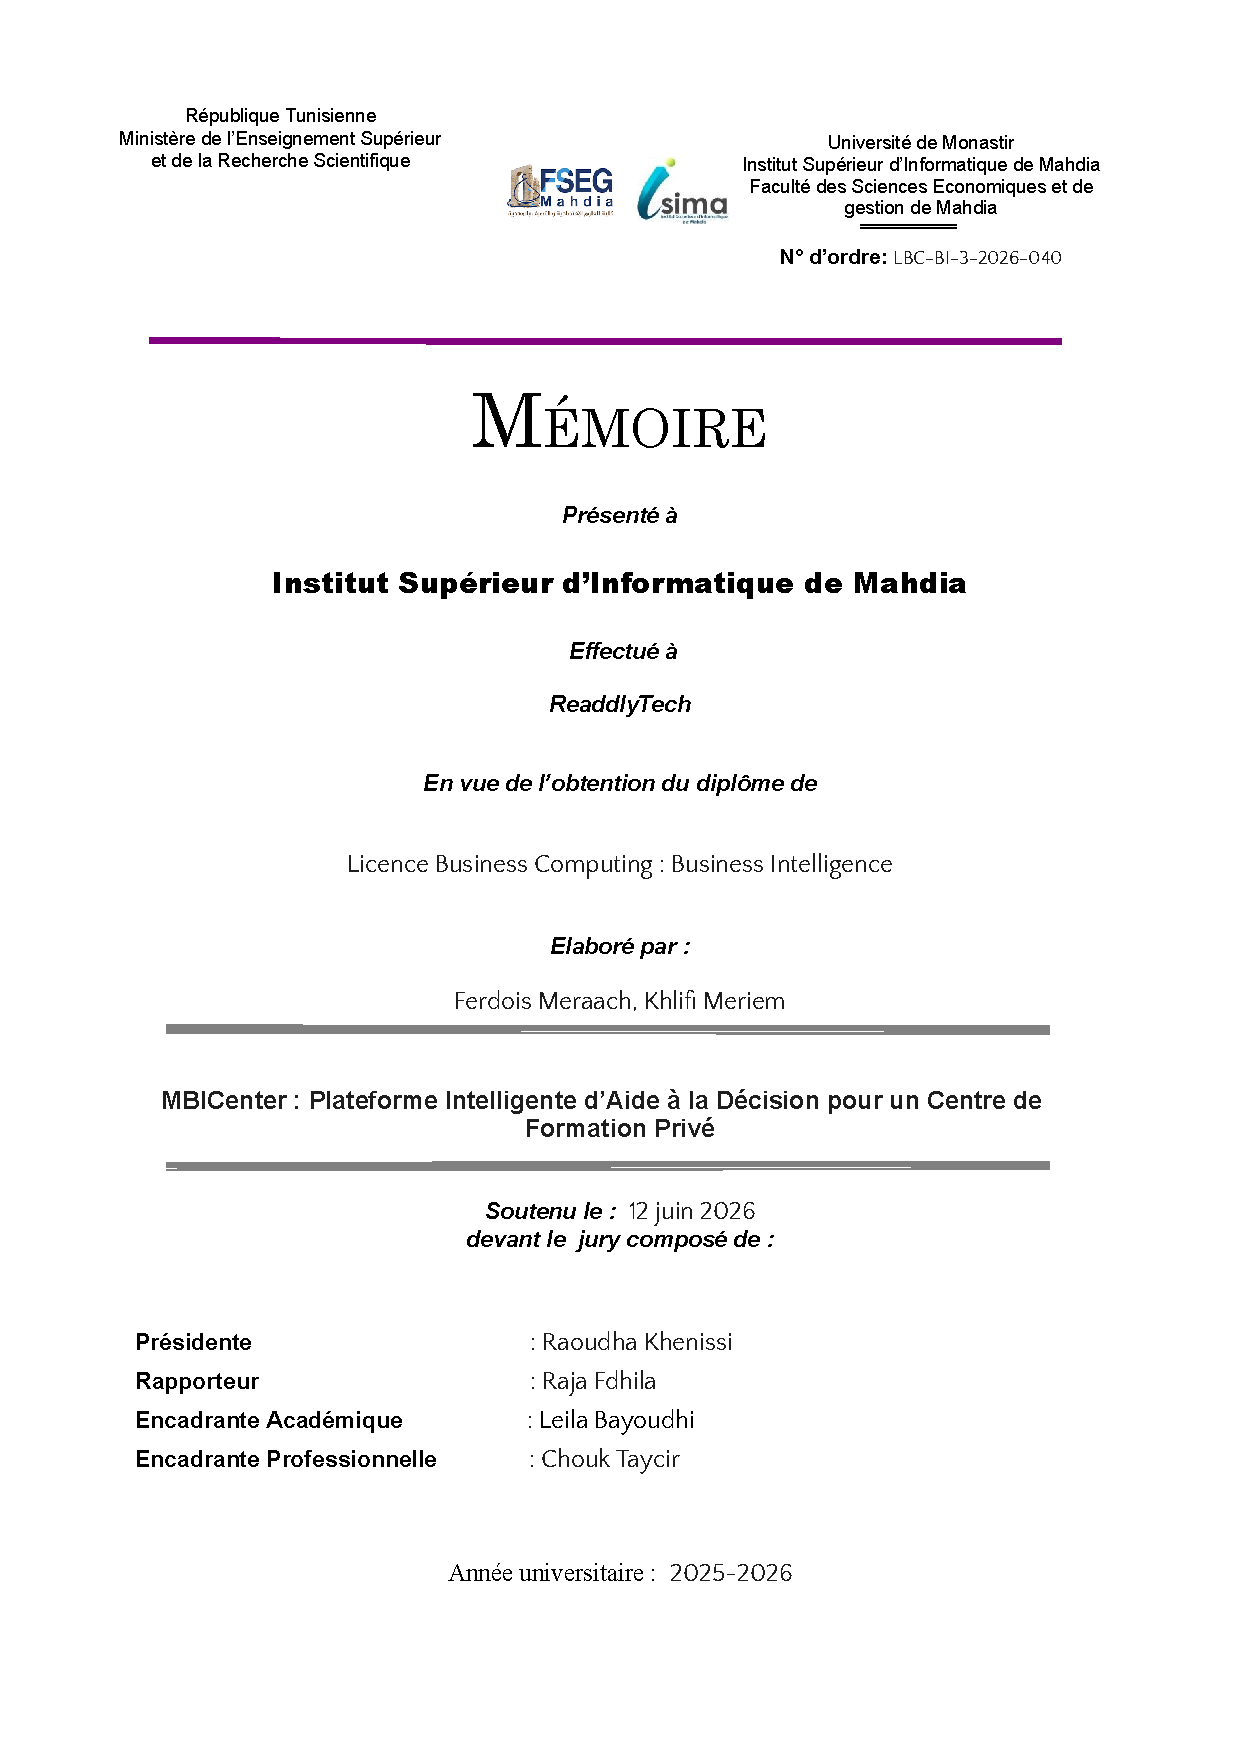
\includepdf{pagedegarde.pdf}
%=========aussi pour la page de remerciment========
%\input{projet/remerciement.tex}
\pagenumbering{roman} % Numérotation des pages en chiffres romains
\clearpage
\thispagestyle{empty}

\begin{center}
    
    {\Huge \bfseries Dédicaces}
\end{center}


\vspace{1cm}
\begin{center}
 \textbf{ Au nom de Dieu, le Tout Miséricordieux, le Très Miséricordieux}
\end{center}
\vspace{1cm}
\textbf{À mes chers parents}, ce travail est avant tout le vôtre. Votre amour inconditionnel, vos sacrifices et votre foi inébranlable en moi m’ont porté à chaque étape de ce
parcours. Vous avez été mes piliers, mes guides, et la source de ma détermination. Merci pour
 chaque encouragement, chaque sourire et chaque moment où vous m’avez rappelé que tout était
possible.

\vspace{0.8cm}
\textbf{À mon cher frère }, à tous les moments d’enfance passés avec toi mon frère, en gage de ma profonde estime pour l’aide que tu m’as apporté. Tu m’as soutenu, réconforté et encouragé. Puissent nos liens fraternels se consolider et se pérenniser encore plus.

\vspace{0.8cm}
À toute ma famille, dont le soutien indéfectible a été un refuge constant, je vous adresse
ma gratitude la plus profonde. Vos conseils, vos prières et votre présence ont donné un sens
particulier à cette aventure. 

\vspace{0.8cm}
À mes amis, ma deuxième famille, vous qui avez partagé mes doutes, mes rires et mes
rêves, merci d’être là. Votre camaraderie, vos encouragements et les souvenirs que nous avons
tissés ensemble ont fait de ce chemin un voyage inoubliable. Ce projet porte aussi l’empreinte
de votre soutien sans faille.

\vspace{0.8cm}
Enfin, je laisse derrière moi ces années universitaires qui m'ont façonné avec un mélange de fierté et de nostalgie, et ce n'est que maintenant que je réalise la valeur de chaque instant devenu souvenir.

\vspace{0.8cm}
Ce rapport est bien plus qu’un aboutissement académique ; il est le reflet de l’amour et de la
force que vous m’avez tous donnés. Du fond du cœur, merci.


\clearpage
\clearpage
\thispagestyle{empty}

\begin{center}
    
    {\Huge \bfseries remerciements}
\end{center}

\vspace{1cm}
La réalisation de ce projet n’aurait pas été possible sans le soutien, les conseils et l’accompagnement de nombreuses personnes auxquelles nous tenons à exprimer notre profonde gratitude.

\vspace{0.8cm}
Tout d’abord, nous tenons à adresser nos plus sincères remerciements à notre encadrante pédagogique, \textbf{Madame Leila Bayoudhi}. votre foi en notre potentiel et votre guidance précieuse tout au long de ce parcours ont été une source d’inspiration constante. votre professionnalisme exemplaire, allié à votre compréhension et votre bienveillance, nous ont permis de surmonter les défis et de donner le meilleur de nous-mêmes.

\vspace{0.8cm}
Nos remerciements vont à nos encadrantes professionnelles, \textbf{Madame Oumaima Halouani} et \textbf{Madame Taycir Chouk}, CEO de \textbf{Readdly Tech}, pour leur soutien indéfectible et leur accompagnement précieux tout au long de notre projet. leurs conseils avisés, leur disponibilité et leur encadrement attentif ont grandement contribué à notre réussite et à notre épanouissement au sein de \textbf{Readdly Tech}.

\vspace{0.8cm}
Nous tenons également à remercier l’ensemble du corps professoral et administratif de   
\textbf{l’Institut Supérieur d’Informatique de Mahdia (ISIMa)} pour leurs efforts inlassables à nous offrir une formation de qualité. votre engagement a été un pilier essentiel dans notre parcours académique.

\vspace{0.8cm}
Enfin, nous adressons nos remerciements aux membres du jury pour l’honneur qu’ils nous font en évaluant ce travail. votre expertise et le temps que vous avez consacré à examiner ce projet sont profondément appréciés.

\vspace{0.8cm}
À toutes et à tous, du fond du cœur, nous vous remercions pour votre contribution à cette aventure, qui restera gravée dans notre mémoire comme une étape marquante de notre parcours.

\clearpage
\chapter*{Résumé} 
Dans un contexte où les centres de formation privés rencontrent des difficultés à piloter efficacement leurs performances en raison de l’absence d’outils décisionnels adaptés, ce projet propose MBICenter, une plateforme intelligente de Business Intelligence dédiée à l’analyse et à l’aide à la décision.

La solution offre aux décideurs des tableaux de bord interactifs, des indicateurs de performance clés et des analyses visuelles permettant un suivi en temps réel des activités du centre.

Le système s’appuie sur une architecture modulaire intégrant un microservice d’intelligence artificielle capable de produire des prédictions stratégiques.

En complément, un module de recommandations basé sur un modèle de langage permet de transformer les résultats analytiques en actions concrètes, facilitant ainsi la prise de décision.

Cette approche vise à accompagner les responsables dans la compréhension de leurs données, la découverte d’insights pertinents et l’amélioration continue de leurs performances, contribuant ainsi à une gestion plus efficace et orientée vers l’avenir.

\textbf{Mots-clés :} Business Intelligence, Machine Learning, aide à la décision, analyse prédictive, centre de formation,Scrum, microservices, Next.js, FastAPI, Nest.js, Supabase.
\clearpage
\dominitoc% 9otlou assna3li sommaire khassa b kol chapitre
\tableofcontents% 9otlou assna3li sommaire globale
 
 \listoffigures% 9otlou assna3li liste figures
  \listoftables%9otlou assna3li liste de tableaux
  \mtcaddchapter  %teb3a sommaire sghira bech tzidheli fi kol chapitre
  %La commande \mtcaddchapter est utilisée avec le package minitoc pour  créer un mini sommaire pour chaque chapitre, affichant les sections et sous-sections qu'il contient.0
 \clearpage
 \clearpage
 \begin{center}
    
    {\Huge \bfseries Liste des acronymes} 
   
\end{center}
\vspace{1.5cm}

\begin{center}
\Large
\begin{tabular}{|c|l|}
\hline
\textbf{BI} & Business Intelligence \\
\hline
\textbf{IA} & Intelligence Artificielle \\
\hline
\textbf{ML} & Machine Learning \\
\hline
\textbf{UML} & Unified Modeling Language \\
\hline
\textbf{ETL} & Extract, Transform, Load \\
\hline
\textbf{ROLAP} & Relational Online Analytical Processing\\
\hline
\textbf{LLM} & Large Language Model \\
\hline
\end{tabular}
\end{center}
 \clearpage
 \pagenumbering{arabic}
\chapter*{Introduction Générale}
% ki nekteb chapter ytalla3li automatiquement chapitre1, ama ena nheb el introduction s'affiche sans le nom de chapitre donc on ajoute *

%ajouter le titre introduction générale dans la table des matières
\addcontentsline{toc}{chapter}{Introduction Générale} 
\markboth{Introduction Générale}{} %définir l'entête de ce chapitre (ki theb taamel entete et pied de page)
L'utilisation des données dans le secteur de l'enseignement et de la 
formation ne date pas d'hier. Les établissements collectent régulièrement 
des informations relatives aux inscriptions, à la participation des 
apprenants, aux résultats des évaluations ainsi qu'aux performances 
pédagogiques.

Au sein des centres de formation privés, ces données jouent un rôle 
central dans le pilotage des activités. Elles concernent aussi bien le 
suivi académique des apprenants que les aspects organisationnels et 
financiers. Cependant, en l'absence d'outils décisionnels adaptés, ces 
données ne sont pas exploitées de manière optimale, ce qui limite 
considérablement leur potentiel stratégique.

Face à cette situation, il devient nécessaire de mettre en place une 
solution décisionnelle capable de centraliser, structurer et analyser 
efficacement ces données. C'est dans cette perspective que s'inscrit notre 
projet \textbf{MBICenter : plateforme intelligente d'aide à la décision 
pour un centre de formation privé}, réalisé dans le cadre de notre stage 
de fin d'études pour l'obtention de la licence en Informatique de Gestion 
à l'Institut Supérieur d'Informatique de Mahdia (ISIMa).

Ce projet a été mené au sein de la startup tunisienne 
\textbf{ReaddlyTech}, spécialisée dans le développement de logiciels et 
de solutions numériques — applications web et mobiles, intégration de 
l'intelligence artificielle et technologies éducatives — dans le but de 
répondre aux besoins croissants en matière de digitalisation et 
d'apprentissage.

L'objectif principal est de concevoir et de développer une plateforme 
décisionnelle permettant de centraliser, d'analyser et de visualiser les 
données issues des activités d'un centre de formation privé. La solution 
offre aux responsables du centre des indicateurs clés de performance (KPIs) 
pour le pilotage stratégique, l'amélioration de la qualité des formations 
et l'optimisation des ressources. Elle intègre également des modèles de Machine Learning et un module de 
recommandations stratégiques basé sur l'intelligence artificielle 
générative, offrant ainsi une aide à la décision proactive et personnalisée.
Afin de présenter ce travail de manière progressive, ce rapport est structuré en six chapitres.

Le chapitre 1, intitulé « Cadre général du projet », présente l'organisme d'accueil, la problématique identifiée ainsi que la solution proposée. 

Ensuite, le chapitre 2 « spécifications des besoins», définit les besoins fonctionnels et non fonctionnels, ainsi que la planification des sprints selon la méthodologie Scrum. 

Par la suite, le chapitre 3 « Conception et environnement Technique », décrit les choix technologiques, l'architecture générale et la conception technique de la solution. 

Les trois derniers chapitres présentent les résultats des trois releases du projet : le chapitre 4 couvre la première release relative à l'authentification et la gestion des utilisateurs. 

Puis, le chapitre 5 traite la deuxième release portant sur la gestion des sessions de formation, l'espace apprenant et l'alimentation des données. 

Enfin, le chapitre 6 est dédié à la troisième release consacrée à la visualisation et à l'analyse des données ainsi qu'au module prédictif et de recommandations stratégiques.
\chapter{Présentation du cadre du projet} 
 \minitoc
 \newpage
\counterwithin{figure}{section}
 
\section{Introduction}
La réussite d’un projet dépend d’une compréhension approfondie de son environnement ainsi que des enjeux qu’il cherche à adresser. Le présent chapitre introductif a pour objectif de poser les fondations de notre projet " Plateforme BI pour l’analyse des performances d’un centre de formation privé ", réalisé au sein de la startup ReaddlyTech.

Dans ce chapitre, nous présentons d’abord l’organisme d’accueil en détaillant ses principaux services dans la section \ref{sec: Présentation de l'organisme d'accueil} . Nous exposons ensuite le contexte du projet dans la section \ref{sec:Contexte de projet}, puis la problématique dans la section \ref{sec:Problématique}. Par la suite, l'analyse de  l’existant dans une section dédiée, en mettant en évidence les études déjà réalisées, leurs limites et critiques, ainsi que la solution que nous proposons. Enfin, nous justifions le choix de la méthodologie adoptée pour ce projet et en expliquons le déroulement.
\section{Présentation de l'organisme d'accueil}
\label{sec: Présentation de l'organisme d'accueil}
ReaddlyTech est une startup EdTech fondée en 2025 et basée à Mahdia. Présente au Canada, aux États-Unis, en Tunisie et en France, elle développe des solutions innovantes destinées aux enfants en difficulté d’apprentissage, notamment l’application Readdly dédiée au soutien de la dyslexie. Afin d’accroître son impact, ReaddlyTech établit des partenariats stratégiques avec des établissements d’enseignement, des thérapeutes et des entreprises du secteur des technologies éducatives. Cette collaboration interdisciplinaire lui permet de répondre à des besoins réels et d’améliorer durablement l’apprentissage ainsi que l’efficacité des organisations éducatives.

Par ailleurs, l’entreprise propose divers services, tels que le développement mobile, l’intelligence artificielle appliquée à l’éducation, la conception d’expériences utilisateurs accessibles et la création d’outils numériques scolaires. Son approche repose sur une ingénierie de qualité, un design centré sur l’utilisateur, l’utilisation du machine learning et des méthodes de développement agiles, afin de concevoir des solutions innovantes à fort impact social et technologique.
\begin{figure}[H]
  \centering
    
\includegraphics[scale=0.3]{project/images/logo (1).png}
  \caption{Organigramme de la startup ReaddlyTech}
\end{figure}


\section{Contexte du projet}
\label{sec:Contexte de projet}
Dans un environnement éducatif de plus en plus axé sur les données, les centres de formation privés produisent un volume important d’informations liées aux activités pédagogiques, administratives et financières .
Cependant, ces données restent souvent dispersées dans différents systèmes ou fichiers, ce qui rend leur exploitation difficile et limite la capacité des responsables à avoir une vision globale et fiable de la performance du centre. \newline
Dans ce contexte, la mise en place d’une plateforme BI dédiée apparaît comme un levier stratégique permettant de centraliser les données, d’analyser les indicateurs clés de performance et de soutenir la prise de décision au sein de l’établissement.
\section{Problématique}
\label{sec:Problématique}
Malgré la disponibilité de nombreuses données opérationnelles, les responsables du centre de formation rencontrent des difficultés à évaluer efficacement les performances pédagogiques, organisationnelles et financières. L’absence d’un outil décisionnel intégré empêche la production rapide d’analyses fiables, complique le suivi des indicateurs clés et limite la capacité d’anticipation face aux dysfonctionnements ou aux opportunités d’amélioration. \newline
La problématique principale consiste donc à savoir comment exploiter efficacement les données disponibles afin de fournir une vision claire, cohérente et dynamique des performances du centre pour faciliter le pilotage stratégique.
\section{Analyse de l’existant}
L'analyse de la situation actuelle est une étape essentielle pour comprendre l’environnement de l’application ainsi que les motivations qui ont conduit à sa conception.
\subsection{Étude de l'existant}
L’analyse de l’environnement technologique actuel des centres de formation met en évidence l’existence de deux catégories principales de solutions numériques : les systèmes de gestion opérationnelle spécialisés et les outils décisionnels généralistes.

D’une part, le marché est majoritairement dominé par des progiciels dédiés à la gestion administrative et pédagogique, tels que\textbf{ Digiforma, Fresh Management, Dendreo et SmartOF}. Ces solutions visent principalement à optimiser les activités quotidiennes des centres, notamment la gestion des inscriptions, la planification des sessions, le suivi des apprenants ainsi que la conformité aux exigences réglementaires, telles que la certification Qualiopi. Elles répondent ainsi efficacement aux besoins opérationnels, mais offrent généralement des fonctionnalités limitées en matière d’analyse stratégique et d’aide à la décision.

D’autre part, certaines organisations adoptent des outils de Business Intelligence généralistes, tels que \textbf{Microsoft Power BI}, \textbf{QlikView} ou les modules décisionnels intégrés à Odoo. Ces solutions permettent la consolidation et l’analyse approfondie des données à travers des tableaux de bord et des indicateurs de performance. Toutefois, leur déploiement requiert souvent des compétences techniques avancées en modélisation, en intégration et en gouvernance des données. Par ailleurs, leur caractère générique peut limiter leur adéquation aux spécificités fonctionnelles du secteur de la formation professionnelle.

Enfin, il reste courant que de nombreux centres reposent encore sur des outils bureautiques traditionnels, notamment des tableurs tels qu’Excel, pour centraliser et exploiter leurs données. Bien que facilement accessibles et flexibles.

\subsection{Critiques de l'existant}
Malgré leur utilité administrative, les solutions existantes souffrent de limites structurelles majeures qui freinent le pilotage stratégique des établissements. Le principal reproche réside dans l'absence d'une véritable analyse décisionnelle avancée, les outils de type ERP se limitant souvent à des rapports statiques sans profondeur analytique. Cette fragmentation empêche une consolidation automatique et fiable des données, rendant le calcul d'indicateurs de performance (KPIs) transversaux — comme la rentabilité réelle par formation ou le taux de complétion précis — particulièrement laborieux. De plus, l'utilisation de systèmes isolés ou de fichiers Excel augmente considérablement le risque d'erreurs humaines, manque de réactivité en temps réel et ne propose aucune perspective évolutive.  ces solutions présentent des limites importantes en termes de fiabilité, de sécurité, d’automatisation et de cohérence des informations, ce qui peut entraver la production d’une vision globale et pertinente pour l'orientation stratégique. En somme, ces outils ne permettent pas d'anticiper les tendances ni de détecter intelligemment les risques, laissant la direction dans une posture réactive plutôt que proactive. C’est précisément pour combler ce fossé entre gestion courante et vision stratégique que notre plateforme BI a été conçue.


\section{Solution proposée}
Face aux limites des solutions existantes, souvent concentrées sur la gestion quotidienne et laissant peu de place à l’analyse stratégique, la solution proposée a pour objectif de fournir aux responsables de centres de formation privés une vision claire et complète de leurs performances pédagogiques et organisationnelles. Elle leur permet de suivre facilement leurs activités, d’identifier rapidement les points à améliorer et de centraliser toutes les informations dans un espace unique, simple à utiliser et intuitif. Cette approche favorise ainsi une prise de décision stratégique fondée sur des données concrètes, fiables et mesurables.

En termes d'innovation, la solution propose des tableaux de bord interactifs et personnalisables, qui s’adaptent au rôle de chaque utilisateur, permettant à chaque acteur (Directeur du centre, résponsable pédagogique, Responsable administratif et financier, Coordinateur des formations) d'accéder aux indicateurs les plus pertinents pour son rôle. Le système intègre également l'automatisation du calcul et de la mise à jour des indicateurs clés de performance (KPI), ce qui réduit le travail manuel et les risques d’erreurs. De plus, l'application offre une visualisation claire et interactive des données grâce à des graphiques analytiques, facilitant l'interprétation et la comparaison des performances dans le temps. Enfin, la plateforme a été pensée pour être simple à utiliser, flexible et évolutive, offrant ainsi un outil adapté aux besoins spécifiques des centres de formation privés, ce qui renforce sa valeur ajoutée par rapport aux outils existants.
\section{Comparaison avec les solutions existantes}
Afin de justifier le choix de notre architecture et de mettre en évidence la valeur ajoutée de notre solution, nous avons réalisé une analyse comparative des outils actuellement disponibles sur le marché. le tableau \ref{tab:comparaison} synthétise les différences fondamentales entre les solutions de gestion spécialisées, les outils de Business Intelligence généralistes et les méthodes traditionnelles (tableurs), par rapport à notre plateforme BI sur-mesure.

    \begin{longtable}{ | p{2.7cm} | p{2.7cm} | p{2.7cm} | p{2.7cm} | p{2.7cm} |}
    \caption{Comparaison de la solution proposée avec les solutions}
    \label{tab:comparaison} \\
        \hline
        \textbf{Critères} & \textbf{Gestion Spécialisée} & \textbf{Outils BI Généralistes} & \textbf{Outils Bureautiques} & \textbf{Notre Solution} \\
        \hline
        \textbf{Exemples} & Digiforma, Dendreo, SmartOF & Power BI, QlikView, Odoo & Excel, Tableurs & \textbf{(Plateforme BI)} \\
        \hline
        \textbf{Objectif} &  Gestion administrative et pédagogique & Analyse décisionnelle des données & Suivi manuel basique & pilotage stratégique du centre \\
        \hline
        \textbf{Centralisation} & Silos(ERP isolé) & Connexion externe & Fragmenté (Fichiers locaux) & Complète\\
        \hline
        \textbf{Interactivité} & Basique(Rapports statiques) & Avancée( dashboards dynamique) & Aucune & Temps Réel (filtres dynamiques) \\
        \hline
        \textbf{Personnalisation des KPIs} & Standards (Génériques) & Modélisation technique & Risque d'erreur (Formules manuelles) & Sur-mesure( taux réussite / abandon; calcul backend) \\
        \hline
        \textbf{Sécurité} & Basique (auth standard) & Bonne (RBAC configurable) & Faible (partage fichiers) & Avancée (JWT, RBAC Guards, bcrypt, HTTPS) \\
        \hline
        \textbf{Automatisation} & Moyenne (docs BPF, relances) & Haute(ETL/ rapports auto)  & Aucune & Totale(import/ nettoyage/ calculs) \\
        \hline
        \textbf{Évolutivité} & Lourde &Complexe & Limitée & Scalable \\
        \hline
        \textbf{Coût \& Complexité} & Licences annuelles élevées & Licences élevées; complexe modélisation  & Gratuit; très complexe/ maintenance & Faible(open tech); déploiement simple scalable\\
        \hline
    \end{longtable}
L'examen du tableau comparatif \ref{tab:comparaison} permet de mieux comprendre pourquoi les outils de formation traditionnels sont insuffisants pour une gestion efficace. Leurs principaux inconvénients résident dans la fragmentation de l'information et la réactivité. Notre solution centralise toutes les données dans un emplacement sécurisé et permet un suivi en temps réel des indicateurs. Contrairement aux méthodes traditionnelles, elle est spécifiquement conçue pour le secteur de la formation et propose des indicateurs pertinents pour les responsables. Ceci permet de passer d'une gestion administrative basique à un véritable outil d'aide à la décision. De plus, l'architecture choisie ouvre la voie à des analyses plus poussées, conférant ainsi au centre de formation un avantage concurrentiel significatif.
\section{Méthodologie de travail }
Afin d’assurer une gestion efficace et flexible du projet, nous avons opté pour la méthodologie Agile Scrum pour encadrer et organiser le déroulement des différentes phases de développement.
 \subsection{Les méthodologies agiles}
Face à un environnement professionnel en constante évolution, la méthode Agile est devenue incontournable pour les équipes cherchant à gagner en flexibilité et en efficacité. Conçue à l’origine pour le développement logiciel, elle s’étend aujourd’hui à de nombreux domaines, du marketing à la gestion d’opérations.
Son efficacité repose sur des sprints courts, une collaboration étroite entre les parties prenantes et une adaptation continue aux priorités du projet. En mettant l’accent sur l’amélioration progressive et des livraisons régulières, elle permet aux équipes d’optimiser leur productivité tout en répondant aux exigences du marché.
La méthode Agile est une approche de gestion de projet qui privilégie l’adaptabilité, la collaboration et la livraison rapide de solutions. Contrairement aux méthodes classiques comme le Waterfall ou le cycle en V, elle repose sur des cycles courts appelés sprints et une amélioration continue basée sur les retours utilisateurs.
L’approche Agile n'est pas un cadre unique, mais un terme générique qui englobe une large gamme de méthodologies, y compris Scrum(Gestion de projet basée sur des principes) , Kanban (met l'accent sur la visualisation du flux de travail, la limitation du travail en cours et l'apprentissage et l'amélioration continus) et Extreme Programming (XP)(qui aide les équipes de développement logiciel à fournir des logiciels de haute qualité tout en restant réactives aux exigences des clients). La figure ci-dessous illustre les étapes à suivre dans le cycle de vie Agile :
\begin{figure}[H]
  \centering
    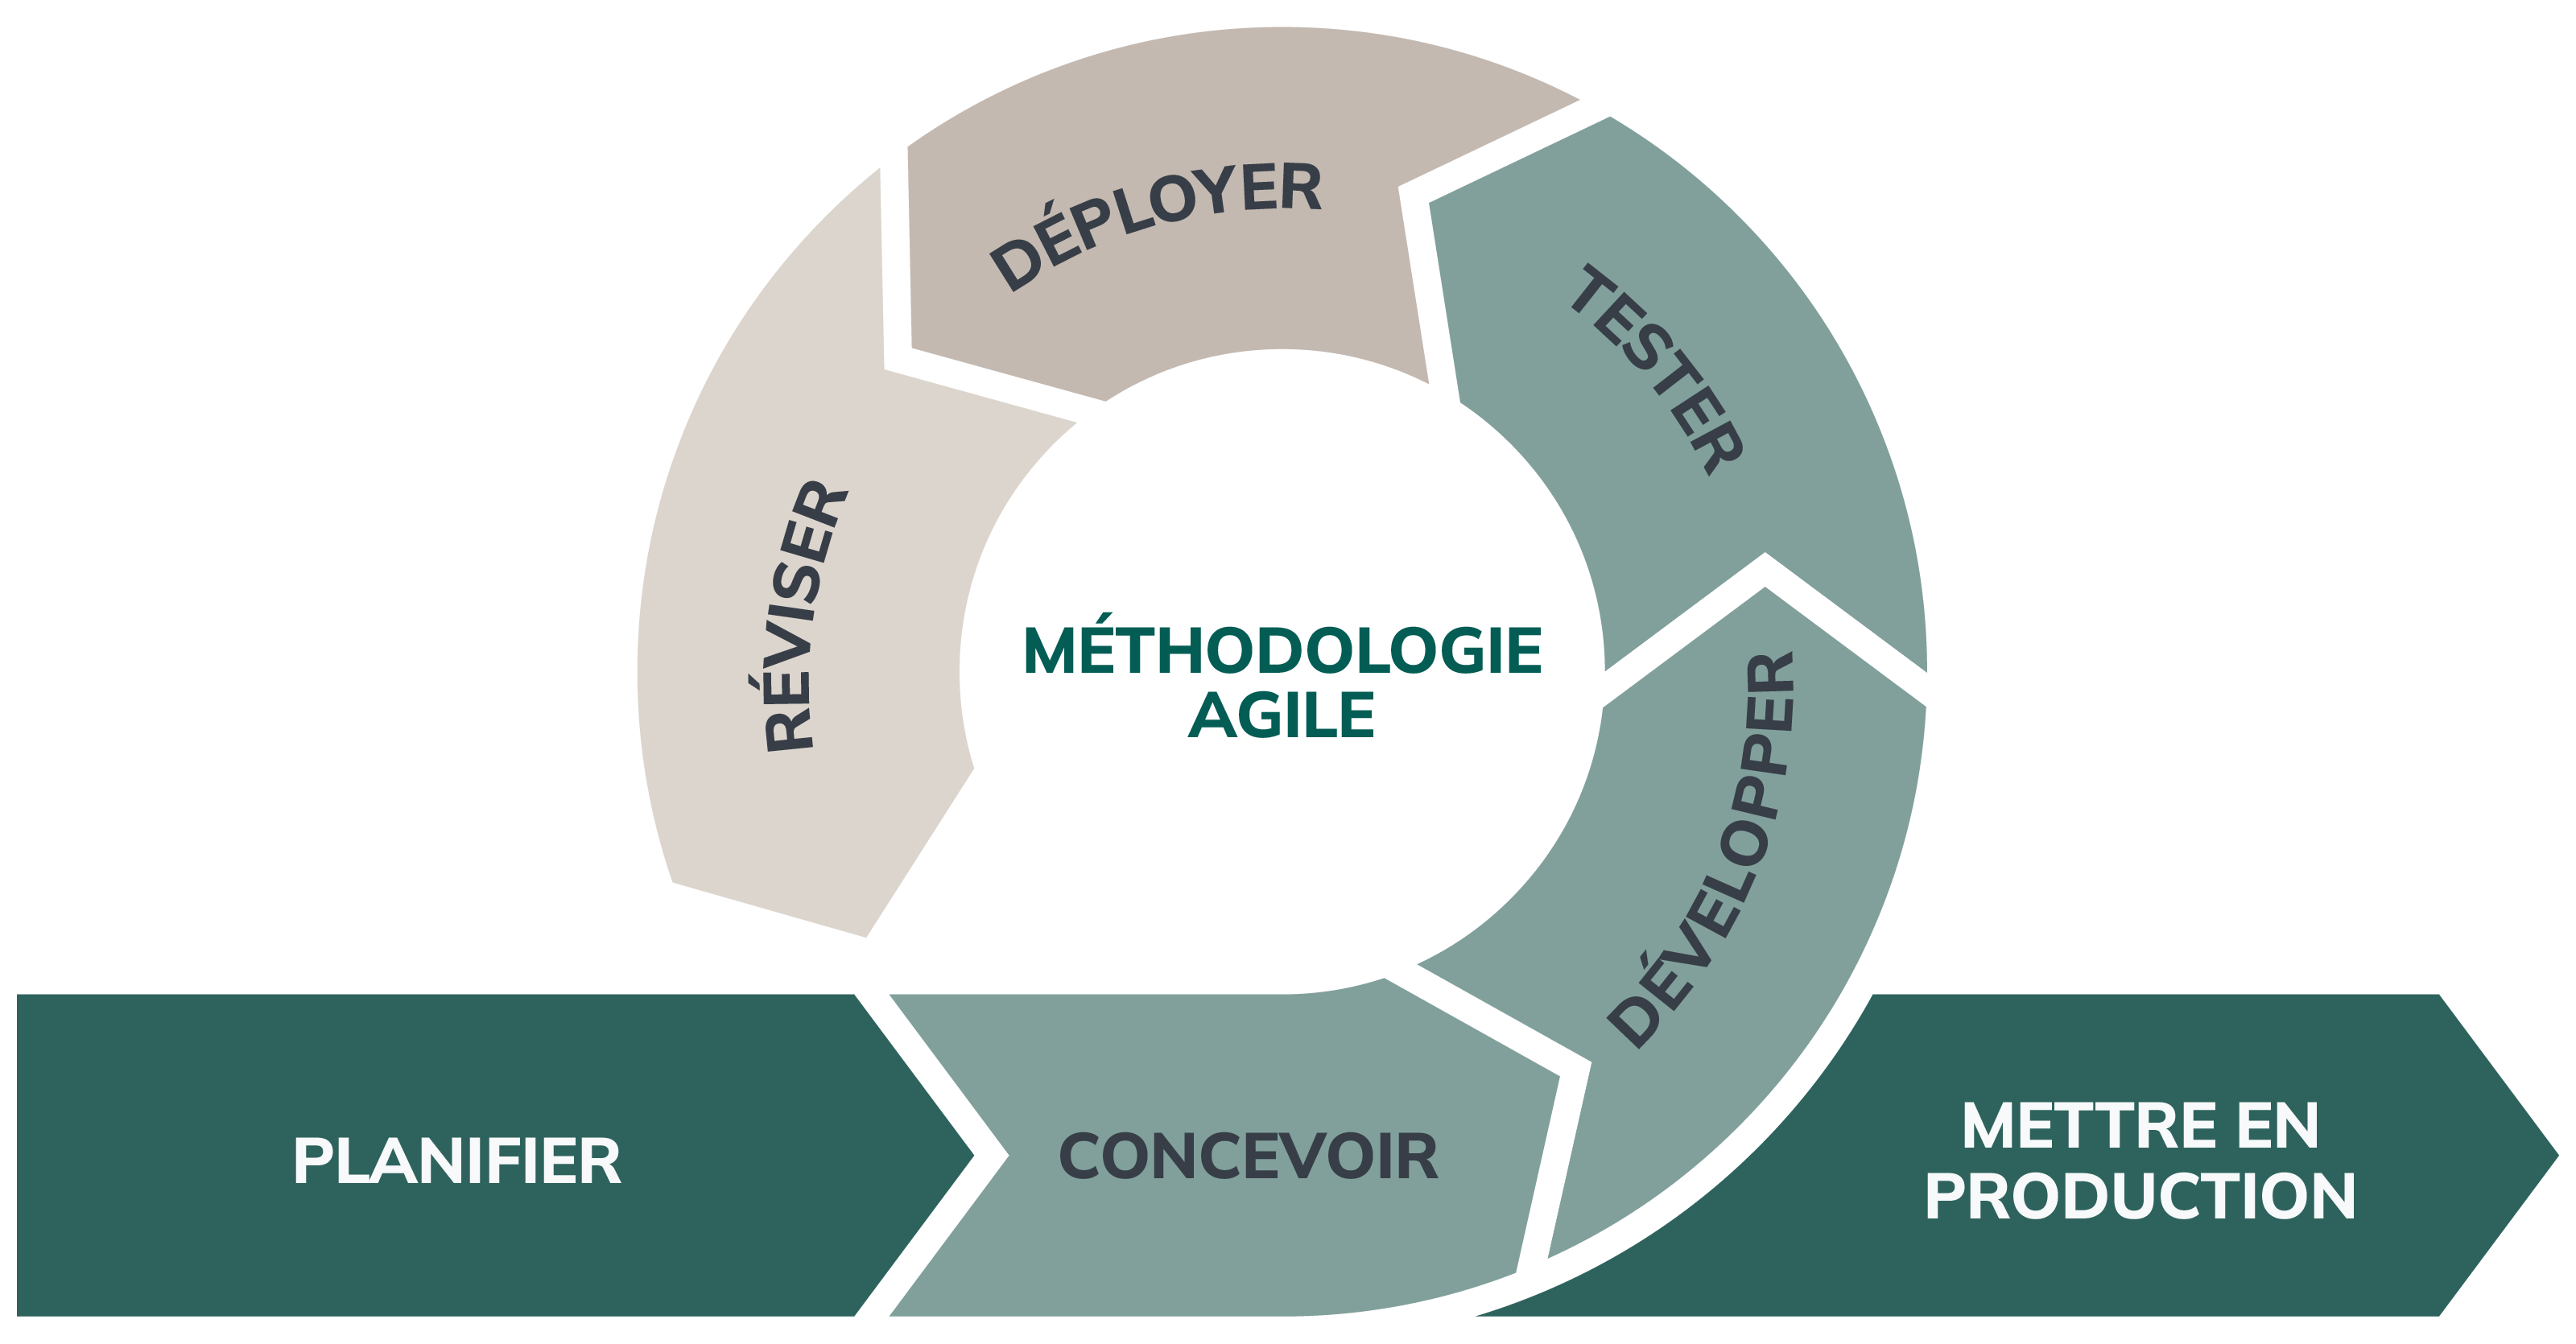
\includegraphics[scale=0.1]{project/images/Agile.png}
  \caption{Processus de méthodologie agile}
\end{figure}

\subsection{La méthodologie SCRUM}
Le framework \textbf{Scrum} repose sur une organisation du travail en cycles courts appelés \textbf{sprints}. Ces cycles, généralement d’une durée de deux semaines, permettent à l’équipe de produire à la fin de chaque itération un livrable exploitable appelé incrément. Chaque sprint possède une durée fixe, un objectif précis (Sprint Goal) ainsi qu’un périmètre défini à travers le Sprint \textbf{Backlog}.

Au début de chaque sprint, une réunion de planification (\textbf{Sprint Planning}) est organisée. Lors de cette réunion, l’équipe sélectionne, à partir du Backlog produit, les éléments qu’elle s’engage à réaliser durant le cycle en cours. Ces éléments constituent le Backlog de sprint. Le \textbf{Product Owner}, responsable de la vision du produit et de la gestion du Backlog produit, collabore avec l’équipe afin de clarifier les priorités et les attentes.

Durant le sprint, l’équipe de développement composée généralement de trois à huit membres travaille à transformer les besoins exprimés en fonctionnalités opérationnelles. Le \textbf{Scrum Master} veille au respect du cadre Scrum et facilite la collaboration au sein de l’équipe. Chaque jour, un \textbf{Daily Scrum} d’une durée de 15 minutes est organisé afin de synchroniser les membres, inspecter l’avancement des travaux et identifier d’éventuels obstacles.

À la fin du sprint, une \textbf{Sprint Review} est tenue pour présenter l’incrément réalisé et vérifier si l’objectif du sprint a été atteint. Cette réunion permet de recueillir les retours du client ou des parties prenantes, même si ces derniers ne font pas directement partie de l’équipe Scrum. Enfin, une rétrospective est organisée afin de prendre du recul, analyser le déroulement du sprint et identifier des axes d’amélioration pour les cycles suivants.

Ainsi, Scrum s’appuie sur les principes de transparence, d’inspection et d’adaptation, garantissant un processus itératif et évolutif centré sur l’amélioration continue et la création de valeur, comme l’illustre la figure 1.8.2 

\begin{figure}[H]
  \centering
    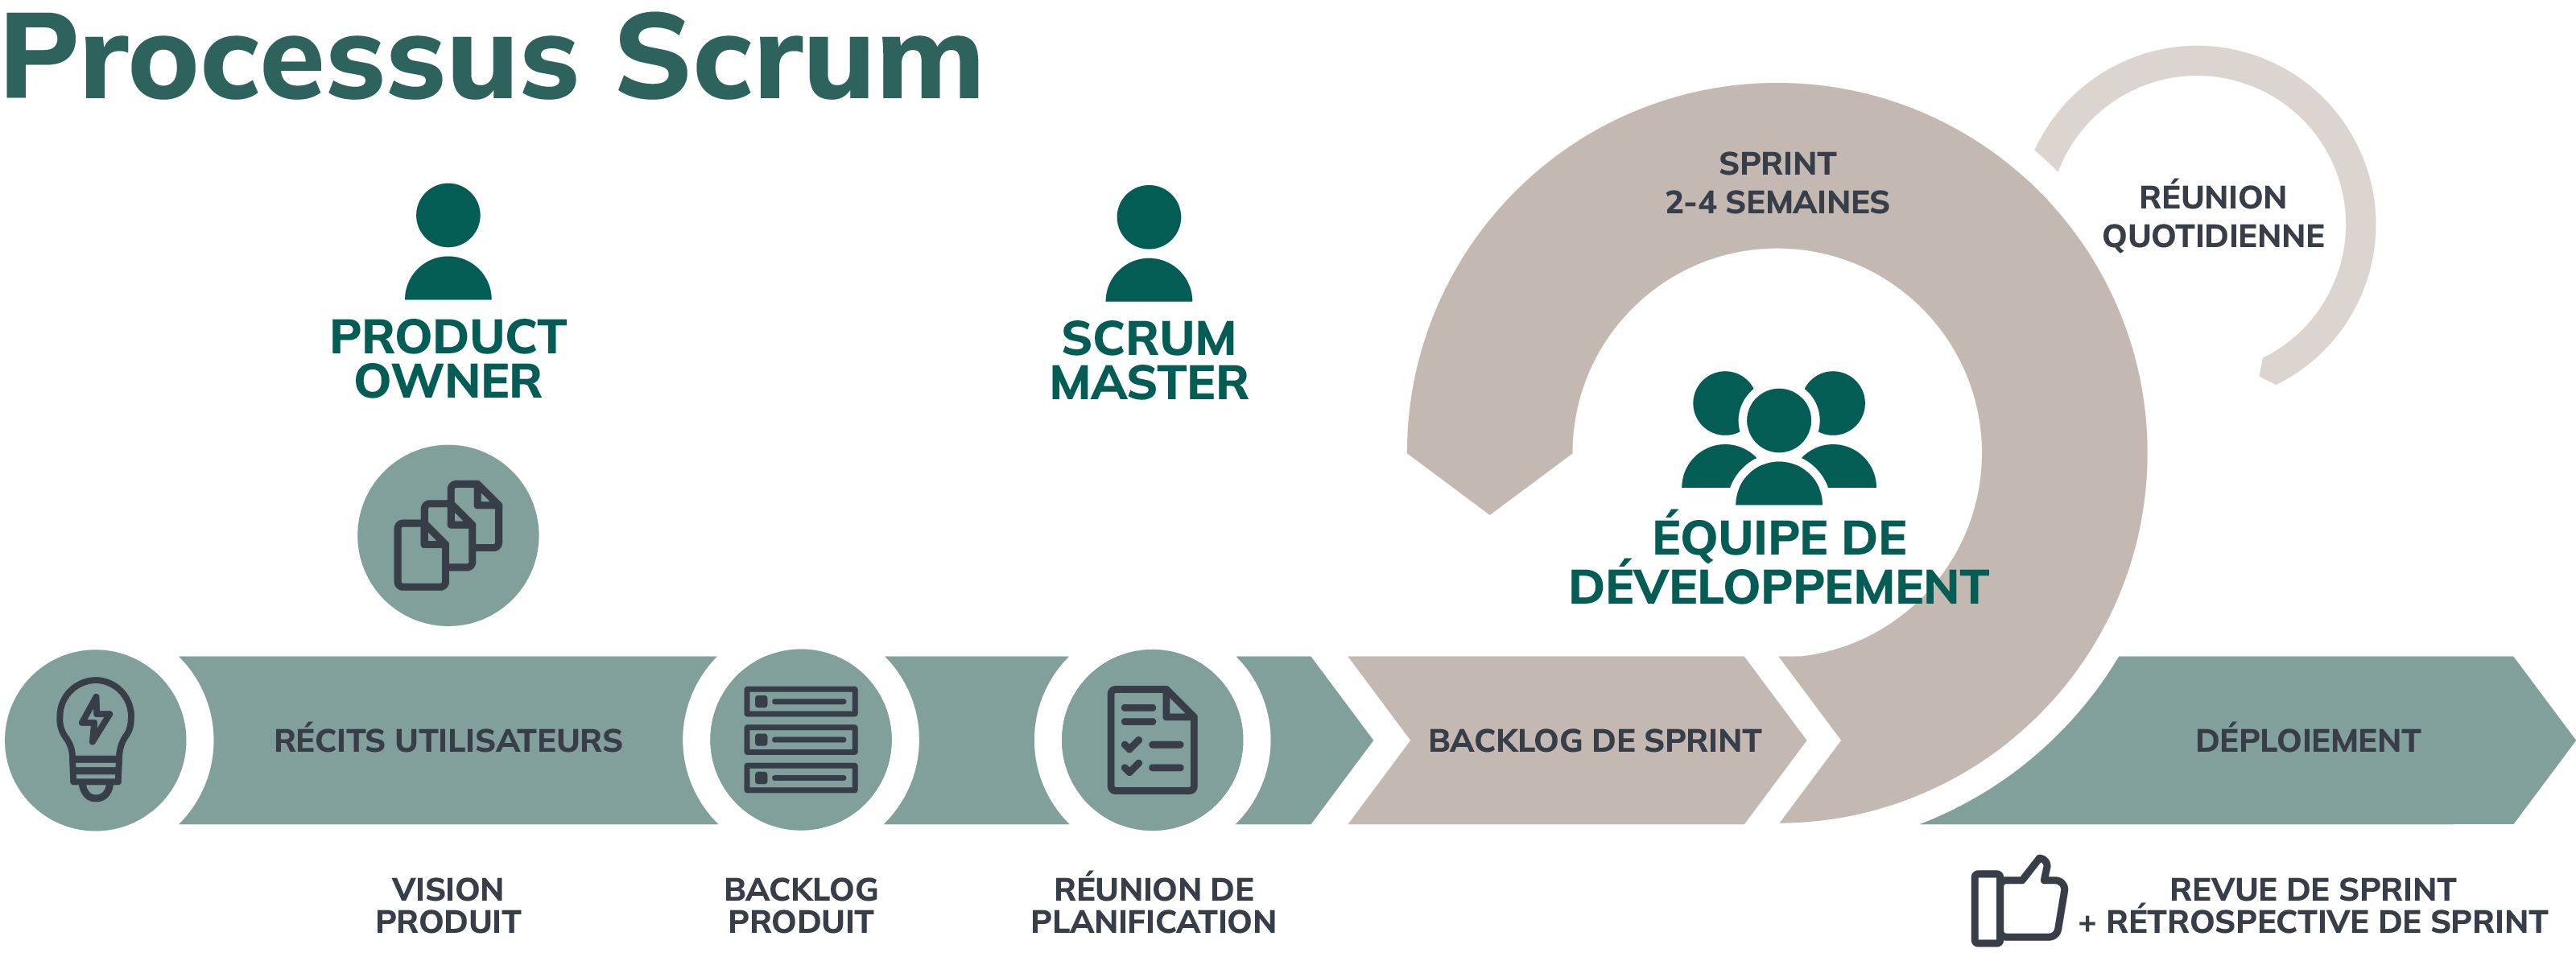
\includegraphics[scale=0.1]{project/images/scrum_agile.png}
  \caption{ Processus de la méthodologie SCRUM agile}
\end{figure}


\section{Conclusion}
Ce premier chapitre a permis de poser les bases de notre projet en présentant l'organisme d'accueil, son contexte et les défis auxquels il fait face. À travers l'étude de l'existant, sNous avons analysé les outils utilisés et mis en évidence leurs principales limites , ce qui nous a permis de proposer des solutions concrètes et adaptées. Pour mener ce travail à bien, nous avons opté pour la méthodologie Scrum Agile, qui nous offre la flexibilité et l'agilité nécessaires pour avancer efficacement tout en restant à l'écoute des besoins. Forts de ces bases solides, nous sommes maintenant prêts à passer à la conception et à la mise en œuvre de notre solution.




 








\chapter{Spécification des besoins} 
 \minitoc
 \newpage
 \counterwithin{figure}{chapter}
 \section{Introduction}
 Après avoir posé les bases et défini le cadre général de notre projet,ce deuxième chapitre constitue l'étape charnière de notre projet, dédiée à la compréhension approfondie des enjeux et à l'organisation du développement. Nous commençons par la capture des besoins dans la section \ref{cap:Capture des besoins}, en identifiant les acteurs clés du centre de formation ainsi que leurs attentes concrètes, tant sur le plan des fonctionnalités que de la fiabilité du système. Nous procédons ensuite à la modélisation des besoins dans la section \ref{cap:Modélisation des exigences} pour traduire ces attentes en une structure visuelle claire. Enfin, nous présentons le pilotage du projet avec Scrum dans la section \ref{cap:Pilotage du projet avec Scrum}, qui définit l’organisation des tâches à travers le backlog ainsi que le rythme de développement en sprints, afin de garantir une collaboration fluide et efficace.

\section{Capture des besoins}
\label{cap:Capture des besoins}
Cette section identifie les acteurs clés du projet et détaille leurs besoins, tant en termes de fonctionnalités que d'exigences de qualité, afin de comprendre les défis de chaque utilisateur et de concevoir un outil de gestion utile à leur quotidien.


\subsection{Identifications des acteurs}
Chaque acteur possède des missions et des attentes spécifiques au sein du centre de formation, allant de la direction stratégique au suivi des cours. Le tableau \ref{tab:Acteurs du système et leurs rôles} présente ainsi les profils retenus et leurs rôles respectifs au sein du système.

\begin{table}[h] 
\centering
\caption{Acteurs du système et leurs rôles}
\label{tab:Acteurs du système et leurs rôles}
\begin{tabular}{|p{4.5cm}| p{11cm}|}
\hline
\textbf{Acteur} &  \textbf{Description} \\
\hline
Directeur & Décideur stratégique du centre, pilote l'établissement et définit la stratégie de développement \\
\hline
Responsable Pédagogique & Garant de la qualité des formations, supervise les programmes, les formateurs et le suivi des apprenants\\
\hline
Responsable Financier & Gère les aspects financiers, la facturation, les paiements et le suivi budgétaire du centre \\
\hline
Administrateur Système &Assure l’administration globale du système, ainsi que la gestion des utilisateurs et des ressources.\\
\hline
Apprenant &Consulte ses propres résultats, suit l'avancement de son parcours et gérer ses inscriptions \\
\hline

\end{tabular}

\end{table}
\subsection{Spécifications des besoins fonctionnels}
Cette section présente les besoins fonctionnels de la plateforme en fonction des différents acteurs, en mettant en évidence les fonctionnalités attendues pour chaque utilisateur selon son rôle. 

\textbf{Besoins fonctionnels de l’acteur « Directeur »}

Le tableau \ref{tab:Besoins fonctionnels de l’acteur « Directeur »} présente les besoins du Directeur, orientés vers l’analyse stratégique de l'établissement.
\begin{table}[H]
\centering
\caption{Besoins fonctionnels de l’acteur « Directeur »}
\label{tab:Besoins fonctionnels de l’acteur « Directeur »}
\begin{tabular}{|p{4.5cm}| p{11cm}|}
\hline
\textbf{Fonctionnalité} & \textbf{Description} \\
\hline
Vue d'ensemble & Consulter un tableau de bord consolidé des performances globales. \\
\hline
Comparaison temporelle  & Analyse comparative multidimensionnelle et temporelle des performances \\
\hline
Analyse multicritère & Analyse des performances selon différents critères.\\
\hline
\end{tabular}
\end{table}

\textbf{Besoins fonctionnels de l’acteur « Responsable pédagogique »}

\vspace{0.3cm}

Le tableau \ref{tab:Besoins fonctionnels de l’acteur « Responsable pédagogique »} présente les besoins du Responsable Pédagogique.

\begin{table}[H]
\centering
\caption{Besoins fonctionnels de l’acteur « Responsable pédagogique »}
\label{tab:Besoins fonctionnels de l’acteur « Responsable pédagogique »}
\begin{tabular}{|p{4.5cm}| p{11cm}|}
\hline
\textbf{Fonctionnalité} & \textbf{Description} \\
\hline
Suivi des apprenants &
Consulter les informations relatives aux apprenants et suivre leur progression. \\
\hline
Analyse des performances &
Analyser les résultats globaux des apprenants et évaluer leur niveau de réussite. \\
\hline
Suivi des formations &
Consulter et analyser l’état d’avancement des formations. \\
\hline
Évaluation des formateurs &
Évaluer les performances des formateurs à partir des résultats obtenus. \\
\hline
Gestion des sessions de formation &
Planifier et organiser les sessions de formation. \\
\hline
Consultation des alertes &
Consulter les alertes liées aux anomalies ou aux situations critiques. \\
\hline
\end{tabular}
\end{table}

\textbf{Besoins fonctionnels de l’acteur «Responsable financier »}

\vspace{0.3cm}

Le tableau \ref{tab:Besoins fonctionnels de l’acteur « Responsable financier »} présente les besoins du Responsable Financier


\begin{table}[H]
\centering
\caption{Besoins fonctionnels de l’acteur « Responsable financier »}
\label{tab:Besoins fonctionnels de l’acteur « Responsable financier »}
\begin{tabular}{|p{4.5cm}| p{11cm}|}
\hline
\textbf{Fonctionnalité} & \textbf{Description} \\
\hline
Gestion des inscriptions & Analyser le flux d'inscriptions mensuel pour prévoir les besoins de facturation. \\
\hline
Calcul des coûts & consulter les coûts liés aux formateurs (honoraires) et aux ressources pour calculer la marge par session.\\
\hline
Suivi des encaissements & Visualiser les montants payés et les montants restants à percevoir.\\
\hline
Analyse de la rentabilité  &  évaluer la rentabilité des formations et des sessions en comparant les revenus générés aux coûts associés, afin d’identifier les activités les plus performantes et celles à optimiser. \\
\hline
\end{tabular}
\end{table}


\textbf{Besoins fonctionnels de l’acteur « Administrateur système »}

\vspace{0.3cm}

Le tableau \ref{tab:Besoins fonctionnels de l’acteur « Administrateur »} présente les besoins de l’Administrateur, centrés sur la gestion des utilisateurs et la maintenance technique du système 
\begin{table}[H]
\centering
\caption{Besoins fonctionnels de l’acteur « Administrateur système  »}
\label{tab:Besoins fonctionnels de l’acteur « Administrateur »}
\begin{tabular}{|p{4.5cm}| p{11cm}|}
\hline
\textbf{Fonctionnalité} & \textbf{Description} \\
\hline
Gestion des utilisateurs & Création et administration des comptes \\
\hline
Gestion des rôles (RBAC) & Attribution des permissions et accès restreints\\
\hline
Gestion des ressources  & Ajout et mise à jour des ressources\\
\hline
 Collecte des données  & Importation manuelle ou automatique des sources (inscriptions, formateurs, etc.)\\
\hline
Traitement des données  & Supervision du nettoyage, validation et structuration des données.\\
\hline
\end{tabular}
\end{table}

\textbf{Besoins fonctionnels de l'Apprenant}

\vspace{0.3cm}

Le tableau \ref{tab:Besoins fonctionnels de l’acteur « Apprenant »} présente les besoins de l’Apprenant. Bien que la plateforme soit principalement orientée décisionnel pour les responsables, l’intégration d’un espace apprenant permet d’améliorer l’engagement, la transparence et le suivi individuel des performances.

\begin{table}[H]
\centering
\caption{Besoins fonctionnels de l’acteur « Apprenant »}
\label{tab:Besoins fonctionnels de l’acteur « Apprenant »}
\begin{tabular}{|p{4.5cm}| p{11cm}|}
\hline
\textbf{Fonctionnalité} & \textbf{Description} \\
\hline
 Consultation de progression& Visualiser son propre taux de complétion de la formation \\
\hline
Accès aux résultats  & Consulter ses notes et ses évaluations finales de manière sécurisée\\
\hline
  Planning et calendrier & Accéder à son emploi du temps personnalisé (dates, lieux, noms des formateurs)\\
\hline
\end{tabular}
\end{table}



\textbf{Besoins fonctionnels du module IA}

\vspace{0.3cm}

Le tableau \ref{tab:Besoins fonctionnels de l’acteur « Module IA »} synthétise les besoins fonctionnels du module Intelligence Artificielle, associant chaque fonctionnalité prédictive à son acteur métier, sa description et ses flux de données.
\begin{table}[H]
\centering
\caption{Besoins fonctionnels de l’acteur « Module IA »}
\label{tab:Besoins fonctionnels de l’acteur « Module IA »}
\begin{tabular}{|p{4.5cm}| p{11cm}|}
\hline
\textbf{Fonctionnalité} & \textbf{Description} \\
\hline
 Alertes sur risques d'abandon &  Analyse prédictive des profils apprenants pour détecter les risques d'abandon et notifier le responsable pédagogique en temps utile.\\
\hline
Prévision des revenus  & Projection budgétaire basée sur l'historique financier et les tendances d'inscription pour accompagner la planification du responsable financier.\\
\hline
  Prévision des inscriptions & Estimation du volume futur des inscriptions pour permettre au directeur d'anticiper les besoins en ressources.\\
\hline
  Prédiction des sessions déficitaires & Prédit les sessions susceptibles d’être déficitaires . Cette analyse permet au responsable financier d’anticiper les pertes et de prendre des décisions financières plus éclairées.\\
\hline
Recommandations stratégiques & Synthèse intelligente des données multi-sources pour proposer au directeur des actions prioritaires et améliorer la performance globale.\\
\hline
\end{tabular}
\end{table}










\subsection{Spécifications des besoins non fonctionnels}

Afin d’assurer la protection des données et fournir un service robuste, le respect des critères suivants est obligatoire :

\noindent\textbf{Performance:} Assurer des temps de réponse rapides pour les tableaux de bord et un traitement efficace des données, tout en supportant un nombre élevé d’utilisateurs simultanés.
\vspace{0.3cm}

\noindent\textbf{Sécurité:} Garantir un haut niveau de sécurité grâce à un mécanisme d’authentification robuste, un contrôle d’accès basé sur les rôles et une protection des données sensibles.

\vspace{0.3cm}
\noindent\textbf{Évolutivité:} Concevoir une solution capable de s’adapter à l’augmentation du volume de données et du nombre d’utilisateurs, tout en facilitant l’ajout de nouvelles fonctionnalités.

\vspace{0.3cm}
\noindent\textbf{Ergonomie:} Offrir une interface intuitive, simple à utiliser et facile à comprendre, assurant une expérience utilisateur fluide.

\vspace{0.3cm}
\noindent\textbf{Compatibilité:} Assurer la compatibilité avec les principaux navigateurs web et permettre une intégration fluide avec les autres systèmes via des APIs standardisées.

\vspace{0.3cm}
\noindent\textbf{Maintenabilité:} Garantir un code propre, structuré et bien documenté, accompagné de mécanismes de journalisation pour faciliter la maintenance et les évolutions.

\vspace{0.3cm}
\noindent\textbf{Fiabilité:} Assurer un fonctionnement stable et continu du système grâce à une gestion efficace des erreurs et des mécanismes de sauvegarde.
\section{Modélisation des exigences}
\label{cap:Modélisation des exigences}
La modélisation des exigences constitue une étape essentielle pour comprendre le fonctionnement du système et la manière dont les différents acteurs interagissent avec ses fonctionnalités. Pour cela, un diagramme de cas d’utilisation global est utilisé afin de représenter de manière synthétique ces interactions et de structurer visuellement les exigences identifiées. Ce diagramme offre une vue d’ensemble claire, facilitant la compréhension des rôles de chaque utilisateur et du flux des actions, tout en préparant efficacement la conception technique à venir.

\noindent La figure \ref{fig:diagrammme de cas d'utilisation globale} présente le diagramme de cas d’utilisation global, illustrant de manière synthétique les rôles de chaque acteur et les principales actions possibles dans le système.

\begin{figure}[H]
  \centering
    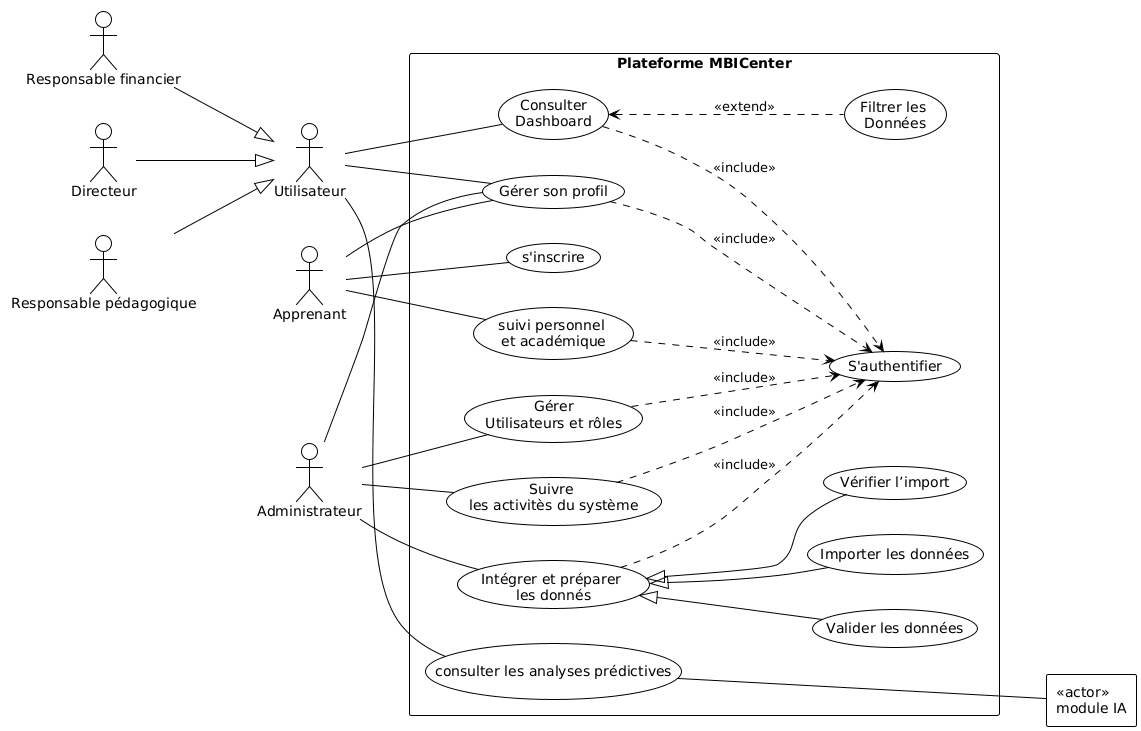
\includegraphics[scale=0.3]{project/images/XLNBRjD05Dr7oZzSkWb8f6fIAIeeYcgI097wW9PqWIf5KtkIZZGUcvbnH4MHsF89x5WshFa3_mbVmXaxiLCdRRE8VEyzz_sOGsEPjaaewODabayZ7VB9cz5av4twKHXBRdczzinUyv1JB9bGzLgz9ldKaer8YzcrfK1exbiHPQ863TB5L2ZX61HmGyotFD46tpHZYNyDUs15cdREk8aZPT.png}
  \caption{ Diagramme de cas d'utilisation globale}
  \label{fig:diagrammme de cas d'utilisation globale}
\end{figure}


\section{Pilotage du projet avec Scrum}
\label{cap:Pilotage du projet avec Scrum}
Dans le cadre de la gestion agile du projet, nous avons opté pour la méthodologie Scrum, qui permet une meilleure organisation des tâches et une priorisation progressive des besoins à travers un backlog produit structuré.

\subsection{Équipe et rôle}
Le bon déroulement et la réussite du projet dépendent d’une répartition efficace des rôles au sein de l’équipe, chacun apportant sa contribution spécifique

\begin{itemize}[label=\textbullet]
  \item \textbf{Product Owner}: Mme Taycir Chouk
  \item \textbf{Scrum Master}: Mme Leila Bayoudhi
  \item \textbf{Development Team }: Mme Mariem khlifi, Mme ferdaws maraach
\end{itemize}




\subsection{Le Backlog du produit}
Le Backlog produit regroupe l’ensemble des fonctionnalités de la plateforme sous forme de User Stories comme indiqué par le tableau \ref{tab:backlog_produit}. Chaque User Story décrit une fonctionnalité du point de vue de l’utilisateur final et est classée par priorité  selon la méthode MoSCoW, qui classe les éléments indispensables (Must), importantes (Should), optionnelles (Could) et non prévues pour cette version (Won’t), afin de réaliser d’abord les éléments les plus importants.
 
\small
\begin{longtable}{|p{1cm}|p{4cm}|p{10cm}|p{1.5cm}|}
\caption{Backlog produit}
\label{tab:backlog_produit} \\
\hline
\textbf{ID} & \textbf{Fonctionnalité} & \textbf{User Story} & \textbf{Priorité} \\
\hline
\endfirsthead
\hline
\textbf{ID} & \textbf{Fonctionnalité} & \textbf{User Story} & \textbf{Priorité} \\
\hline
\endhead

% --- US01 : Authentification ---
\multirow{3}{*}{\textbf{1}} & \multirow{3}{*}{\textbf{Authentification}}
& En tant qu'utilisateur, je veux m'authentifier de manière sécurisée pour accéder aux données selon mon rôle. & M \\
\cline{3-4}
& & En tant qu'apprenant, je veux pouvoir créer un compte sur la plateforme afin de m'inscrire à une formation. & M \\
\cline{3-4}
& & En tant qu'utilisateur, je veux pouvoir réinitialiser mon mot de passe oublié afin de retrouver l'accès à mon espace personnel en toute sécurité. & M \\
\hline

% --- US02 : Gestion des utilisateurs ---
\multirow{3}{*}{\textbf{2}} & \multirow{3}{*}{\textbf{Gestion des utilisateurs}}
& En tant qu'administrateur, je veux gérer les utilisateurs (activer, désactiver, modifier) et traiter les inscriptions. & M \\
\cline{3-4}
& & En tant qu'administrateur, je veux attribuer et gérer les rôles et permissions pour contrôler les accès. & M \\
\cline{3-4}
& & En tant qu'administrateur, je veux modifier et configurer les profils personnels des utilisateurs. & M \\
\hline

% --- US03 : Gestion des sessions de formation---
\multirow{4}{*}{\textbf{3}} & \multirow{4}{*}{\textbf{\shortstack[1]{Gestion des sessions \\ de formation}}}
& En tant que responsable pédagogique, je veux organiser et gérer les sessions de formation afin d'assurer le suivi et le bon déroulement des formations. & M \\
\hline

% --- US04 : Espace apprenant ---
\multirow{4}{*}{\textbf{4}} & \multirow{4}{*}{\textbf{Espace apprenant}}
& En tant qu'apprenant, je veux être redirigé automatiquement vers la page d'inscription lors de ma première connexion, afin de rejoindre une session avant d'accéder aux autres modules. & M\\
\cline{3-4}
& & En tant qu'apprenant, je veux voir un résumé de mes statistiques (formations inscrites, sessions à venir, moyenne générale) afin d'avoir une vue d'ensemble de mon parcours. & S\\
\cline{3-4}
& & En tant qu'apprenant, je veux consulter la liste des formations auxquelles j'ai participé, afin de suivre mon avancement. & S\\
\cline {3-4}
& & En tant qu'apprenant, je veux consulter les formations disponibles auxquelles Je n’ai pas encore participé, afin de découvrir de nouvelles opportunités d'apprentissage. & S\\
\cline {3-4}
& &  En tant qu'apprenant, Je veux participer à une session disponible d’une formation, afin de rejoindre une promotion active. & M\\
\cline {3-4}
& &  En tant qu'apprenant, je veux annuler ma participation à une session, afin de me désinscrire si mes disponibilités changent. & S\\
\cline{3-4}
& & En tant qu'apprenant, je veux consulter l'historique de toutes mes inscriptions passées et actuelles, afin de garder une trace de mon parcours. & C\\
\cline{3-4}
&& En tant qu'apprenant, je veux consulter mon emploi du temps complet (filtrable par semaine ou par mois), afin d'organiser mon agenda. & S\\
\cline{3-4}
& & En tant qu'apprenant, je veux consulter la synthèse de toutes mes notes par formation, afin d'évaluer mes performances globales. & C\\
\cline{3-4}
&& En tant qu'apprenant, je veux consulter la liste paginée de tous mes paiements (filtrables par formation, session ou date), afin de suivre ma situation financière. & S\\
\cline{3-4}
&& En tant qu'apprenant, je veux attribuer une note et un commentaire à une formation que j'ai suivie, afin de partager mon retour d'expérience. & C \\
\hline
% --- US05 : Alimentation des données ---
\multirow{4}{*}{\textbf{5}} & \multirow{4}{*}{\textbf{Alimentation des données}}
& En tant qu'administrateur, je veux importer les données brutes (raw data) pour centraliser les informations. & M \\
\cline{3-4}
& & En tant qu'administrateur, je souhaite que le système détecte automatiquement les erreurs dans les données importées afin de garantir leur qualité. & M \\
\cline{3-4}
& & En tant qu'administrateur, je veux valider ou rejeter les données importées afin que seules les données correctes soient stockées dans la base de données. & M \\
\cline{3-4}
& & En tant qu'administrateur, je souhaite charger les données validées dans la base de données afin qu'elles puissent être utilisées pour l'analyse et la production de rapports. & S \\
\hline
% --- US06 : Visualisation et analyse des données --- 
\multirow{6}{*}{\textbf{6}} & \multirow{6}{*}{\textbf{\shortstack[l]{Visualisation et \\ analyse des données}}} & En tant qu’utilisateur interne, je veux analyser les données du centre afin de comprendre les performances des activités. & M \\
 \cline{3-4}
& & En tant qu’utilisateur interne, je veux visualiser les indicateurs de performance sous forme de graphiques afin de suivre l’évolution des résultats. & M \\
\cline{3-4} & & En tant qu’utilisateur interne, je veux consulter des tableaux de bord afin de suivre les KPIs du centre. & M \\
\cline{3-4} & & En tant qu’utilisateur interne, je veux filtrer les données afin d’affiner mes analyses selon différents critères. & S \\ 
\cline{3-4} & & En tant que utilisateur interne, je veux exporter des rapports afin de partager les analyses et les résultats du centre. & M \\
\cline{3-4} & & En tant qu'utilisateur interne, je veux recevoir des notifications et alertes afin d'être informé en temps réel de tout événement important lié au fonctionnement du centre. & S \\ 
\hline


% --- US07 : Module prédictif et recommandations ---
\multirow{4}{*}{\textbf{7}} & \multirow{4}{*}{\textbf{\shortstack[l]{Module prédictif \\ et recommandations}}}
& En tant que responsable pédagogique, je veux recevoir des alertes sur les risques d'abandon générées par l'IA afin d'intervenir rapidement auprès des apprenants en difficulté. & C \\
\cline{3-4}
& & En tant que responsable financier, je veux prévoir les revenus afin de planifier le budget. & C \\
\cline{3-4}
&& je veux pouvoir prédire la probabilité de survenue de sessions déficitaires afin d'anticiper les risques financiers pour optimiser la rentabilité de l'entreprise. & C\\
\cline{3-4}
& & En tant que directeur, je veux des capacités d'analyse prédictive (prévision des inscriptions) afin d'anticiper les besoins futurs. & C \\
\cline{3-4}
& & En tant que Directeur, je veux accéder à des recommandations stratégiques basées sur l'analyse des données, afin de mieux prioriser les actions, déléguer les responsabilités et améliorer les performances globales de l'établissement. & C \\
\hline
\end{longtable}

\subsection{Planification des sprints}
Après avoir finalisé et ordonné le backlog produit, nous avons procédé à une estimation précise
des durées prévisionnelles de chaque sprint. Suite à une évaluation détaillée de la charge de travail,
nous avons défini 3 versions principales.

\noindent Le tableau \ref{tab:release_planning} présente la répartition détaillée de notre planification des sprints, en soulignant:
\begin{itemize}

  \item  La durée estimée de chaque sprint.
  \item Les principales fonctionnalités à développer.
  \item Les objectifs spécifiques de chaque version
 \end{itemize}
\begin{table}[H]
\centering
\caption{Planification des sprints}
\label{tab:release_planning}
\begin{adjustbox}{width=\textwidth}
\begin{tabular}{|c|c|l|c|}
\hline
\textbf{Release ID} & \textbf{Sprint} & \textbf{Nom du Sprint} & \textbf{Estimation (jours)} \\
\hline

\multirow{2}{*}{Release 1} 
& 1 & Authentification & 10 \\
\cline{2-4}
& 2 & Gestion des utilisateurs & 10 \\
\hline

\multirow{3}{*}{Release 2} 
& 3 & Gestion des sessions de formation & 10 \\
\cline{2-4}
& 4 & Espace apprenant & 10 \\
\cline{2-4}
& 5 & Alimentation des données & 10 \\
\hline

\multirow{2}{*}{Release 3} 
& 6 & Visualisation et analyse des données & 10 \\
\cline{2-4}
& 7 & Module prédictif et recommandations & 10 \\
\hline

\end{tabular}
\end{adjustbox}
\end{table}

\section{Conclusion} 


Ce chapitre nous a permis de définir précisément "pour qui" et "comment" nous allons construire cette solution. En comprenant les besoins des utilisateurs et en structurant notre méthode de travail agile, nous avons désormais une vision claire du projet. Forts de ces bases solides, nous pouvons maintenant aborder, dans le chapitre suivant, le choix des technologies et la conception technique qui permettront de transformer ces besoins en une plateforme réelle.
\chapter{ Conception et environnement Technique} 
 \minitoc
 \newpage
 \counterwithin{figure}{chapter}

 \section{Introduction}
 Ce chapitre présente les éléments techniques et conceptuels ayant guidé la réalisation de la solution. Il introduit le cadre de développement ainsi que les principaux choix adoptés. La section \ref{sec:Environnement de travail} décrit l'environnement de travail et les technologies utilisées. La section \ref{sec:Architecture générale de l'application} présente l'architecture générale du système. La section \ref{sec:Conception technique et modélisation multidimensionnelle} est consacrée à la conception technique et à la modélisation du système, tandis que la section \ref{sec:Conception de l'interface des utilisateurs } traite de la conception de l'interface utilisateur. Enfin, une synthèse des choix effectués clôt ce chapitre afin de préparer la phase d'implémentation.
 \section{Environnement de travail}
 \label{sec:Environnement de travail}
L'environnement de travail regroupe tous les outils, langages et frameworks utilisés pour concevoir, développer et tester une application. Il joue un rôle essentiel pour assurer l'efficacité, la cohérence et la qualité du projet.


\subsection{Outils de développement et modélisation}

\noindent
\begin{minipage}{0.55\textwidth}
\raggedright
\textbf{UML (Unified Modeling Language):} Le Langage de Modélisation Unifié (voir figure \ref{fig:uml_logo}), de l'anglais Unified Modeling Language (UML) \cite{uml_spec}, est un langage de modélisation graphique à base de pictogrammes conçu comme une méthode normalisée de visualisation dans les domaines du développement logiciel et en conception orientée objet.
\end{minipage}
\hfill
 \begin{minipage}{0.4\textwidth}
        \centering
        
\includegraphics[width=0.8\textwidth]{project/images/UML_logo.svg.png}

       \captionof{figure}{Logo UML}
       \label{fig:uml_logo}
    \end{minipage}

\noindent
\begin{minipage}{0.55\textwidth}
\raggedright
\textbf{Visual Studio Code :} (ou VS Code) \cite{vscode_docs}, est un éditeur de code source gratuit, léger et performant, développé par Microsoft. Il est très populaire pour le développement web et logiciel grâce à sa rapidité, la coloration syntaxique, la saisie semi-automatique intelligente, les extraits de code, les outils de restructuration de code et le contrôle de version Git intégré (voir figure \ref{fig:vscode_logo}).
\end{minipage}
\hfill
 \begin{minipage}{0.3\textwidth}
        \centering
        
\includegraphics[width=0.7\textwidth]{project/images/image.png}

       \captionof{figure}{logo VsCode}
       \label{fig:vscode_logo}
    \end{minipage}
    
\noindent
\begin{minipage}{0.55\textwidth}
\raggedright
\textbf{Figma :} \cite{figma_docs} est une plateforme de conception graphique vectorielle et de prototypage basée sur le cloud (voir figure \ref{fig:figma_logo}), principalement utilisée pour créer des interfaces utilisateur (UI) et des expériences utilisateur (UX) de sites web et d'applications mobiles. Il permet la collaboration en temps réel, facilitant le travail d'équipe, le design system et le passage de relais aux développeurs.
\end{minipage}
\hfill
 \begin{minipage}{0.3\textwidth}
        \centering
        
\includegraphics[width=0.5\textwidth]{project/images/Figma-logo.svg.png}

       \captionof{figure}{Logo Figma}
       \label{fig:figma_logo}
    \end{minipage}

\noindent
\begin{minipage}{0.55\textwidth}
\raggedright
\textbf{GitHub:} \cite{github_docs} est une plateforme de développement collaboratif qui permet aux développeurs de stocker, gérer et suivre les modifications de leur code source en utilisant Git, un système de gestion de versions distribué (voir figure \ref{fig:github_logo}).
\end{minipage}
\hfill
 \begin{minipage}{0.3\textwidth}
        \centering
        
\includegraphics[width=0.7\textwidth]{project/images/25231.png}

       \captionof{figure}{ Logo GitHub}
       \label{fig:github_logo}
    \end{minipage}

\noindent
\begin{minipage}{0.55\textwidth}
\raggedright
\textbf{Postman :} \cite{postman_docs} est un outil de développement d'API qui permet aux développeurs de tester, déboguer et documenter les API de manière efficace. Son interface conviviale simplifie le processus de test des requêtes HTTP et de collaboration au sein des équipes (voir figure \ref{fig:postman_logo}).
\end{minipage}
\hfill
 \begin{minipage}{0.3\textwidth}
        \centering
        
\includegraphics[width=0.7\textwidth]{project/images/unnamed.png}

 \captionof{figure}{ Logo Postman}
       \label{fig:postman_logo}
    \end{minipage}
    

\subsection{Langages de programmation}
Cette section présente les principaux langages de programmation utilisés dans le développement du projet.

\noindent
\begin{minipage}{0.55\textwidth}
\raggedright
\textbf{JavaScript :} \cite{javascript_mdn} est un langage de programmation interprété (voir figure \ref{fig:javascript_logo}), dynamique et polyvalent, principalement utilisé pour rendre les pages web interactives. Il est aujourd'hui un pilier du développement web moderne et fonctionne aussi bien côté client (navigateur) que côté serveur via Node.js.
\end{minipage}
\hfill
 \begin{minipage}{0.3\textwidth}
        \centering
        
\includegraphics[width=0.7\textwidth]{project/images/img_javascript_480.jpg}

 \captionof{figure}{Logo Js}
       \label{fig:javascript_logo}
    \end{minipage}
    
\noindent
\begin{minipage}{0.55\textwidth}
\raggedright
\textbf{TypeScript :} \cite{typescript_docs} représente l'évolution moderne de JavaScript, apportant un système de typage statique qui renforce considérablement la robustesse et la maintenabilité du code (voir Figure \ref{fig:typescript_logo}).
\end{minipage}
\hfill
 \begin{minipage}{0.3\textwidth}
        \centering
        
\includegraphics[width=0.8\textwidth]{project/images/typescript.png}

 \captionof{figure}{Logo TypeScript}
       \label{fig:typescript_logo}
    \end{minipage}

\noindent
\begin{minipage}{0.55\textwidth}
\raggedright
\textbf{Python :} \cite{python_docs} est un langage de programmation de haut niveau (voir figure \ref{fig:python_logo}), interprété et orienté objet, reconnu pour sa syntaxe intuitive et facile à lire. Open source, il est largement adopté pour des domaines variés tels que le développement web, la science des données, l'intelligence artificielle et l'automatisation.
\end{minipage}
\hfill
 \begin{minipage}{0.3\textwidth}
        \centering
        
\includegraphics[width=0.7\textwidth]{project/images/Python-logo-notext.svg.png}
        \captionof{figure}{Logo Python}
        \label{fig:python_logo}
    \end{minipage}


\subsection{Framework et technologies utilisé}
\noindent
\begin{minipage}{0.55\textwidth}
\raggedright
\textbf{Next.js :} \cite{nextjs_docs} est un framework moderne basé sur React, conçu pour faciliter le développement d'applications web complètes (full-stack). Il permet aux développeurs de créer des interfaces utilisateur dynamiques en s'appuyant sur les composants React, tout en bénéficiant de fonctionnalités avancées et d'optimisations intégrées (voir figure \ref{fig:nextjs_logo}).
\end{minipage}
\hfill
 \begin{minipage}{0.3\textwidth}
        \centering
        
\includegraphics[width=0.7\textwidth]{project/images/images (5).png}

 \captionof{figure}{Logo NextJs}
        \label{fig:nextjs_logo}
    \end{minipage}

\noindent
\begin{minipage}{0.55\textwidth}
\raggedright
\textbf{NestJS :} \cite{nestjs_docs} est un framework backend moderne basé sur Node.js et TypeScript (voir figure \ref{fig:nestjs_logo}), offrant une architecture modulaire et évolutive pour le développement d'applications serveur. Il fournit des fondations robustes pour construire des API REST, des microservices ou toute logique métier côté serveur, tout en facilitant la maintenabilité et l'organisation du code.
\end{minipage}
\hfill
 \begin{minipage}{0.3\textwidth}
        \centering
        
\includegraphics[width=0.7\textwidth]{project/images/images (6).png}

 \captionof{figure}{Logo NestJs}
        \label{fig:nestjs_logo}
    \end{minipage}

\noindent
\begin{minipage}{0.55\textwidth}
\raggedright
\textbf{Chart.js :} \cite{chartjs_docs} est une bibliothèque JavaScript open-source (voir figure \ref{fig:chartjs_logo}) qui permet de créer facilement des graphiques interactifs et visuels dans une application web. Elle utilise le canevas HTML5 pour dessiner différents types de graphiques (barres, lignes, camemberts, etc.) et offre des options de personnalisation pour représenter clairement des données.
\end{minipage}
\hfill
 \begin{minipage}{0.3\textwidth}
        \centering
        % TODO: Add Chart.js logo image file (chartjs-logo.png) to project/images/
        
\includegraphics[width=\textwidth]{project/images/chartjs-logo.png}

 \captionof{figure}{Logo Chartjs}
        \label{fig:chartjs_logo}
    \end{minipage}

\subsection{Base de données}
\noindent
\begin{minipage}{0.55\textwidth}
\raggedright
\textbf{PostgreSQL:} \cite{postgresql_docs} est un système de gestion de base de données relationnelle orientée objet, open source et performant, capable de gérer des données complexes. Il privilégie la conformité SQL et l'extensibilité. De plus, il est adapté aux charges de travail OLAP (Online Analytical Processing), ce qui permet d'effectuer des analyses et des traitements avancés sur de grands volumes de données (voir figure \ref{fig:postgressql_logo}).
\end{minipage}
\hfill
 \begin{minipage}{0.3\textwidth}
        \centering
        
\includegraphics[width=0.7\textwidth]{project/images/elephant.png}

 \captionof{figure}{Logo PostgresSql}
        \label{fig:postgressql_logo}
    \end{minipage}
\newline

 \section{Architecture générale de l'application}
  \label{sec:Architecture générale de l'application}
 L'architecture désigne la structure technique qui organise les différents composants de l'application (frontend, backend, base de données, services externes) ainsi que leurs interactions. Elle définit la circulation des données, les modalités de communication entre les composants et l'emplacement ou le mode d'exécution de chaque élément. Dans cette section, nous présentons l'architecture logicielle de notre application. La figure \ref{fig:placeholder} illustre l'architecture générale retenue, laquelle est structurée en trois parties principales. \newline

\begin{figure}[H]
     \centering
     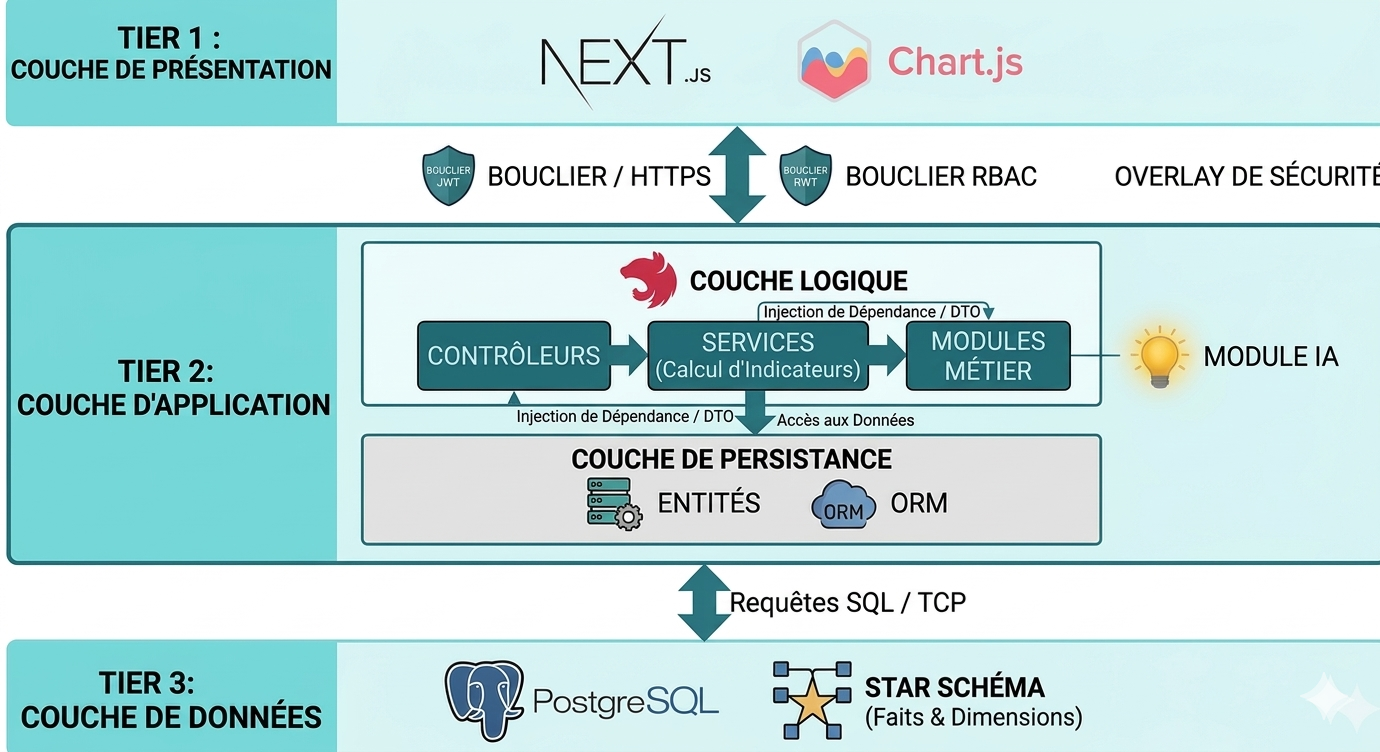
\includegraphics[width=0.8\linewidth]{project/images/Gemini_Generated_Image_jsvpksjsvpksjsvp.png}
     \caption{architecture generale}
     \label{fig:placeholder}
 \end{figure}
 \vspace{0.8cm}
 
\textbf{Tier 1 : Couche de Présentation (Front-end)}\newline
Il représente les interfaces de l'application, c'est-à-dire les éléments avec lesquels l'utilisateur peut interagir. \newline
\textbf{Tier 2 : Couche Application (Back-end)}\newline
Il englobe les fonctionnalités de l'application et leur implémentation. Il est invisible pour les utilisateurs de l'application, mais il assure le dynamisme de celle-ci.

\textbf{communication et securité:} La communication entre le frontend et le backend se fait via des API REST, utilisant des requêtes HTTP pour échanger des données au format JSON. Pour garantir la sécurité de ces échanges, nous avons mis en place une couche de sécurité qui valide les jetons d'authentification (JWT) et vérifie les droits d'accès (RBAC) avant de permettre l'accès aux ressources protégées du backend.

\textbf{Couche logique :} 
représente la partie centrale de l'application où sont implémentées les règles métier. Elle est responsable du traitement des données, de l'exécution des opérations et de la prise de décisions en fonction des besoins fonctionnels.

\textbf{Couche persistence :} Utilise un ORM (Object-Relational Mapping) pour faire le pont entre le code et la base de données, assurant une manipulation fluide des Entities.\newline
\textbf{Tier 3 : Couche de Données (Database)}\newline
Elle englobe la base de données ainsi que les différents mécanismes permettant de manipuler les données de façon sécurisée et efficace.
\newline

\section{Conception technique et modélisation multidimensionnelle}
\label{sec:Conception technique et modélisation multidimensionnelle}
\subsection{Diagramme de classes}
Dans cette section, nous allons explorer la structure logique de la plateforme à travers son diagramme de classes. Ce diagramme permet de visualiser les principales entités du système, leurs attributs et méthodes essentiels, ainsi que les relations qui les lient, offrant ainsi une vue d'ensemble claire de l'architecture du projet.

La figure \ref{fig:diagramme de classe} présente cette modélisation et illustre comment les différentes classes interagissent pour assurer le fonctionnement cohérent de la plateforme.

\begin{figure}[H]
  \centering
    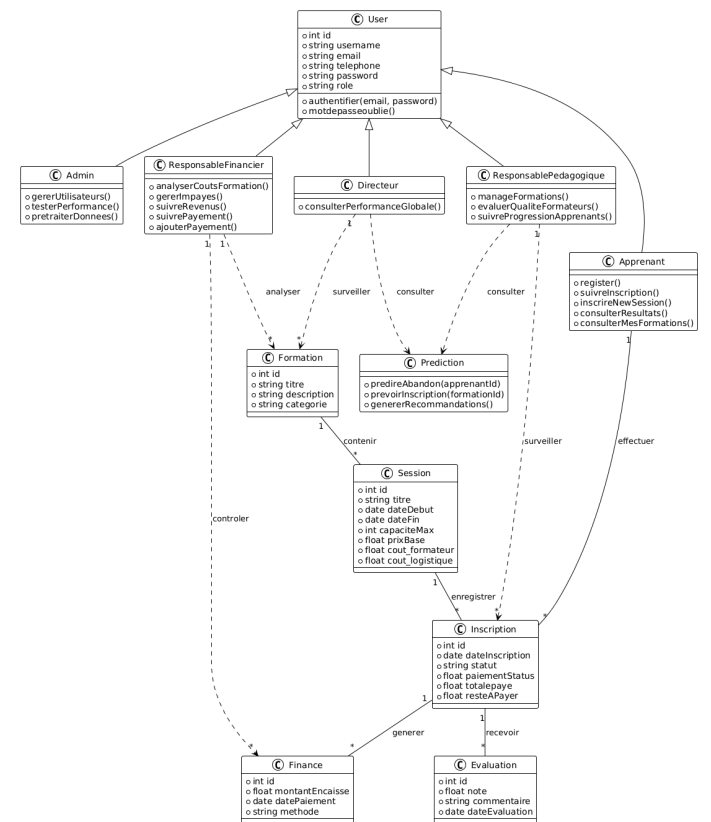
\includegraphics[scale=0.8]{project/images/diagClasse.png}
  \caption{ Diagramme de classe}
  \label{fig:diagramme de classe}
\end{figure}

\subsection{Modélisation décisionnelle}
La modélisation multidimensionnelle est l'étape clé pour structurer les données afin de faciliter l'analyse. Le système repose sur une architecture ROLAP, implémentée à l’aide d’une base de données relationnelle PostgreSQL, en s’appuyant sur un schéma en constellation pour optimiser les requêtes analytiques.

\textbf{ Les Dimensions}\newline Les dimensions représentent les axes d'analyse 

Dim-Temps: Permet d'analyser les données par année, semestre, mois et jour.

Dim-Apprenants: Regroupe les informations sur les profils inscrits (niveau, ville, etc.).

Dim-Formations: Contient les détails des programmes proposés.

Dim-Formateurs: Identifie les intervenants et leurs expertises.

Dim-Sessions: Précise le cadre temporel et physique (ou virtuel) des cours.

\textbf{ Les Faits}\newline
Les faits contiennent les mesures quantitatives (les indicateurs de performance ou KPIs).

Faits-Inscriptions : Analyse le volume des nouveaux inscrits et les flux d'admission.

Faits-Performances : Suit les résultats pédagogiques (notes, taux de réussite).

Faits-Finances : Centralise les données monétaires (revenus, impayés, CA).

Le choix du schéma en étoile se justifie par la simplicité des jointures. Contrairement à un schéma en flocon, il réduit le nombre de tables à interroger, ce qui accélère la génération des graphiques dans le dashboard final.

\section{Conception de l'interface des utilisateurs }
\label{sec:Conception de l'interface des utilisateurs }
La conception des interfaces a débuté par une approche intégrée combinant l'interface utilisateur (UI) et l'expérience utilisateur (UX), essentielles pour une solution intuitive et efficace.
l'utilisation de Figma pour concevoir les interfaces
avant leur développement s'est révélée cruciale. Cette approche a permis de prototyper rapidement les flux utilisateur, tester les interactions, et optimiser le temps de livraison en identifiant
les besoins essentiels. Cette sous-section détaille ces deux aspects
distincts, en s'appuyant sur des bases théoriques et pratiques adaptées au projet.
\subsection{Conception UI/UX}
\textbf{Interface Utilisateur (UI) }\newline
L'interface utilisateur (UI) constitue le principal point d'interaction avec la plateforme décisionnelle, conçue pour offrir une visualisation claire et intuitive des KPIs. Une hiérarchisation efficace met en avant les indicateurs clés sous forme de cartes, complétées par des graphiques interactifs pour analyser les tendances. la typographie a été définie avec la police Inter, largement utilisée dans le projet pour sa modernité et sa lisibilité, garantissant une présentation claire des
texte, Le choix de la palette de couleurs s'est orienté vers des tons \textit{sage} et \textit{cream}, comme illustré dans la Figure \ref{fig:placeholder3}. Ces couleurs ont été sélectionnées pour leur aspect apaisant et professionnel, favorisant une meilleure lisibilité des informations. Toutefois, ce choix reste évolutif et pourra faire l'objet d'ajustements lors de la phase de réalisation, afin d'améliorer davantage l'expérience utilisateur et l'ergonomie de l'interface.
\begin{figure}[H]
     \centering
     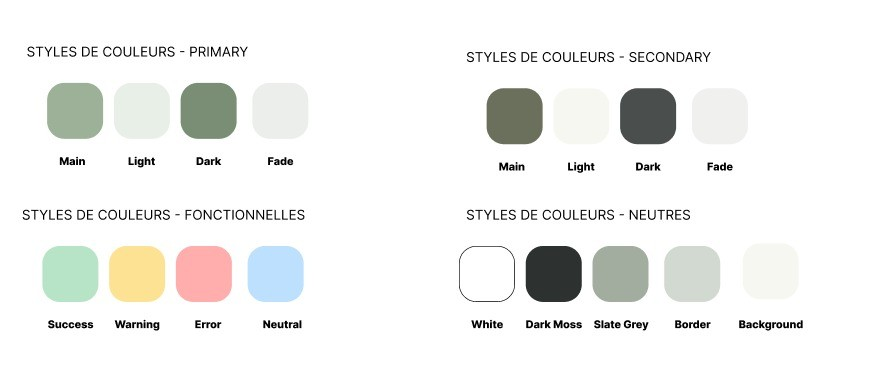
\includegraphics[width=0.8\linewidth]{project/images/WhatsApp Image 2026-03-23 at 9.56.31 PM.jpeg}
     \caption{palette de couleurs suggérée }
     \label{fig:placeholder3}
 \end{figure}
 \vspace{0.8cm}
\textbf{Expérience Utilisateur (UX)}
L'expérience utilisateur (UX) se focalise sur la manière dont les utilisateurs perçoivent et interagissent avec la plateforme décisionnelle, dans le but d'optimiser leur satisfaction et l'efficacité de leur travail. L'organisation de l'information a été pensée pour présenter le contenu et les options de navigation de façon claire et logique, facilitant un accès rapide aux fonctionnalités essentielles. Les interactions sont fluides et cohérentes entre les différents écrans, tandis que les parcours utilisateurs sont conçus pour guider intuitivement l'exploration des données et des KPIs. Ces choix ergonomiques contribuent à une expérience agréable, efficace et adaptée aux besoins d'analyse et de suivi des performances.
\newline

\subsection{Maquettage de l'interface}

Les maquettes présentées dans cette section représentent une première version du design de l'interface.La Figure \ref{fig:placeholder1} montre l'écran de connexion de la plateforme décisionnelle, tandis que la Figure \ref{fig:placeholder2} présente l'interface du Responsable Pédagogique, Elles ont été conçues afin de définir la structure générale des écrans et l'organisation des informations. Des améliorations seront apportées par la suite, notamment en ce qui concerne l'harmonisation et la gradation des couleurs ainsi que l'optimisation de l'ergonomie.

\begin{figure}[H]
     \centering
     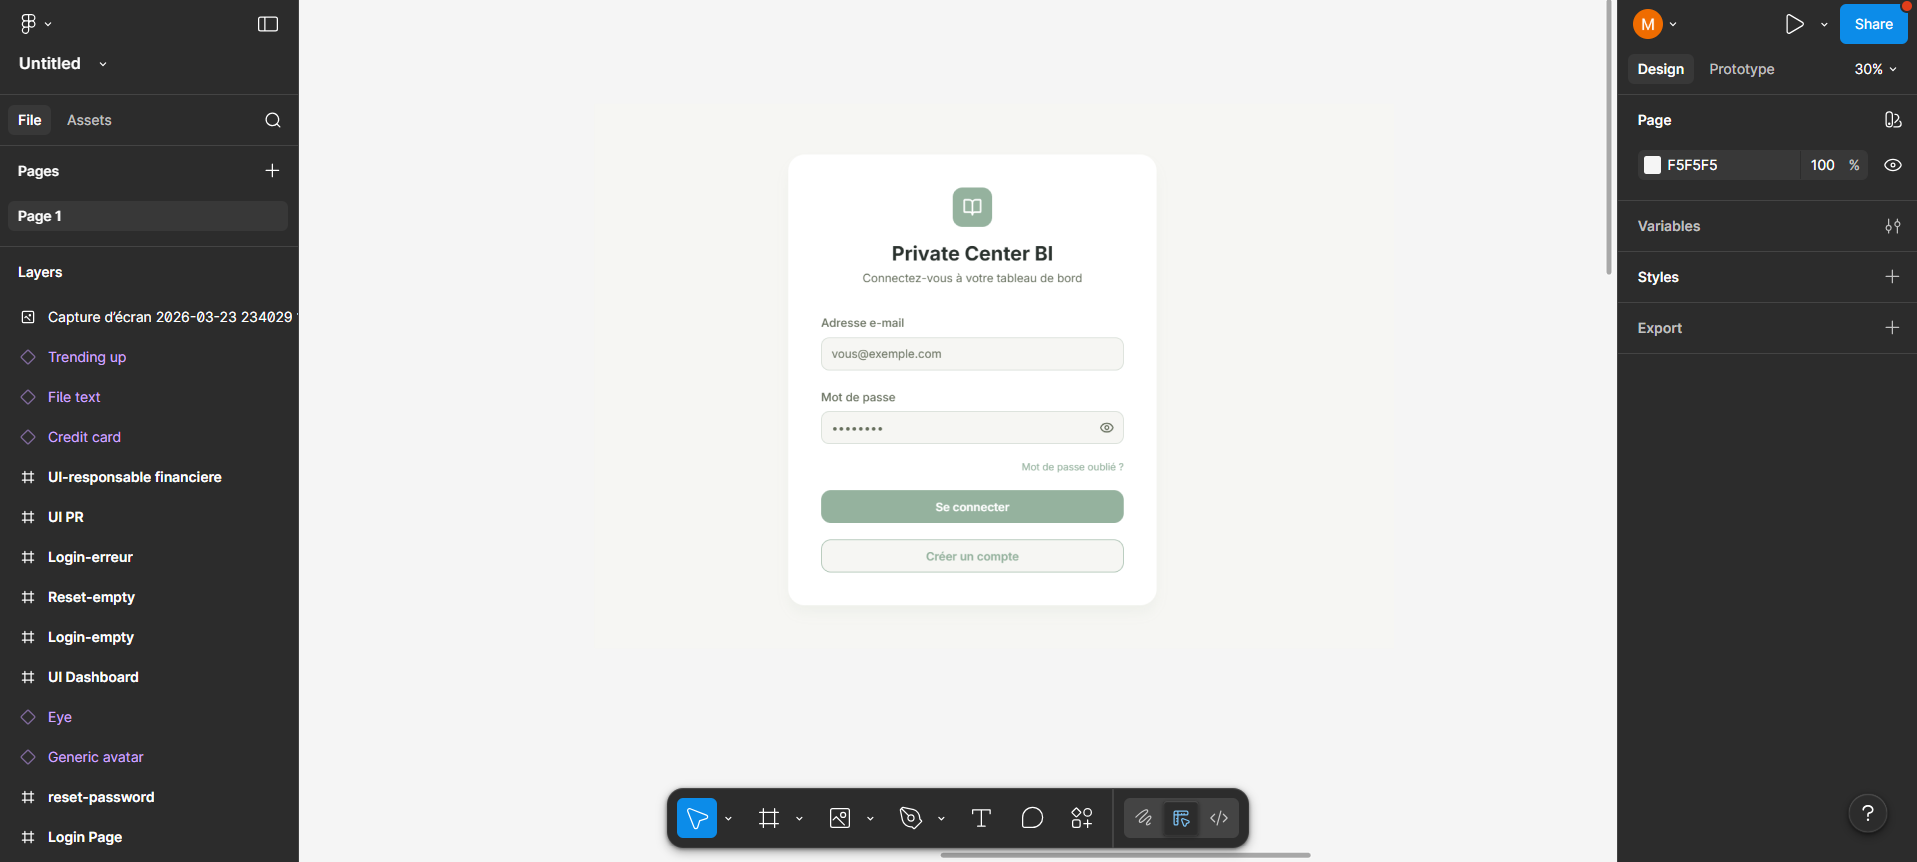
\includegraphics[width=0.8\linewidth]{project/images/Capture d’écran 2026-03-23 234150.png}
     \caption{maquette de l'écran de connexion }
     \label{fig:placeholder1}
 \end{figure}

        \begin{figure}[H]
     \centering
     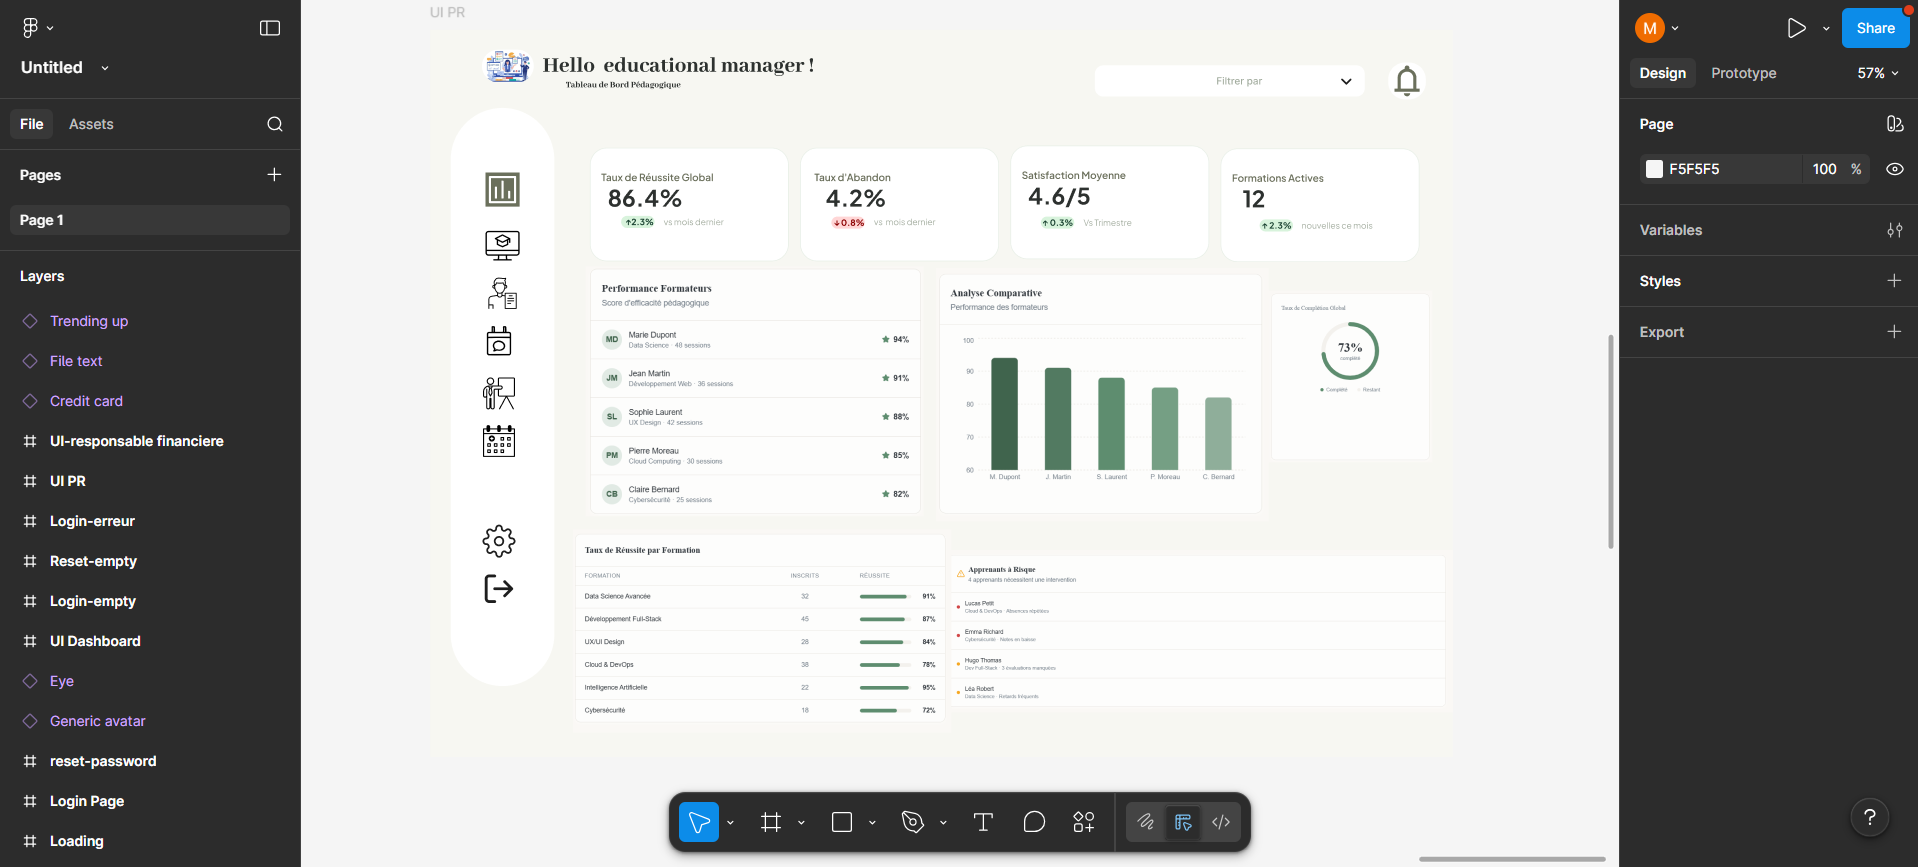
\includegraphics[width=0.8\linewidth]{project/images/Capture d’écran 2026-03-23 232928.png}
     \caption{maquette de l'interface du Responsable Pédagogique}
     \label{fig:placeholder2}
 \end{figure}
 

\section{Conclusion}
En résumé, ce chapitre a permis de définir l'environnement de travail et les technologies choisis pour garantir la performance du système. Nous avons détaillé l'architecture générale ainsi que la conception technique, notamment à travers le diagramme de classes et la modélisation décisionnelle. 
Enfin, l'étude de l'interface utilisateur (UI/UX) et le maquettage ont permis de fixer l'aspect visuel de la plateforme. Ce cadre conceptuel étant validé, nous pouvons maintenant passer à la phase de réalisation de l'application.
\chapter{Release 1:Authentification et gestion des utilisateurs} 
 \minitoc
 \newpage
 \counterwithin{figure}{chapter}
\section{Introduction}
La première release de notre plateforme repose sur la mise en place de fonctionnalités fondamentales, notamment l’authentification et la gestion des utilisateurs, réalisées à travers deux sprints stratégiques.
Ce chapitre décrit de manière structurée le processus de développement adopté, en s’appuyant sur les backlogs ainsi que sur les user stories qui ont guidé la conception et l’implémentation.
Pour chaque sprint, une analyse des cas d’utilisation est présentée, suivie d’une phase de conception illustrée par des diagrammes de séquence, puis d’une phase de réalisation mettant en évidence les interfaces développées.
La section \ref{sec:sprint1-authentification} est consacrée à la sécurisation de l’accès à la plateforme, tandis que la section \ref{sec:sprint2-gestion-utilisateurs} traite de la gestion des utilisateurs et des rôles. Ces deux sprints constituent une base essentielle pour les fonctionnalités analytiques futures.

  \section{Sprint 1: «Authentification»}
  \label{sec:sprint1-authentification}
  Cette section présente les résultats du premier sprint, dédié au développement du module d’authentification de la plateforme. Au cours de ce sprint, les efforts ont été orientés vers la mise en place des fonctionnalités essentielles, notamment l’inscription, la connexion des utilisateurs ainsi que la récupération des mots de passe, tout en intégrant des mécanismes de sécurité basés sur l’authentification et l’autorisation.
  \subsection{Le backlog du sprint 1}
  Dans cette partie, nous présentons le backlog du sprint 1, qui a été élaboré à partir des besoins fonctionnels identifiés pour la fonctionnalité d’authentification. Ce backlog comprend les user stories détaillées, permettant de planifier et de prioriser les tâches à réaliser pendant ce sprint comme le montre le tableau \ref{tab:sprint1_backlog}.
  \begin{table}[H]
\centering
\caption{Backlog du Sprint 1 : Authentification}
\label{tab:sprint1_backlog}
\begin{tabular}{|c|p{4cm}|p{10cm}|c|}
\hline
\textbf{ID} & \textbf{Fonctionnalité} & \textbf{User Story} & \textbf{Priorité} \\
\hline
\multirow{3}{*}{1} & \multirow{3}{*}{Login / S'inscrire} 
& En tant qu’utilisateur, je veux me connecter de manière sécurisée pour accéder à mon espace selon mon rôle. & M \\
\cline{3-4}
& & En tant qu’étudiant, je veux pouvoir créer un compte sur la plateforme afin que mon accès soit validé par l’administrateur. & M \\
\cline{3-4}
& & En tant qu’utilisateur, je veux pouvoir réinitialiser mon mot de passe oublié afin de retrouver l’accès à mon espace personnel. & M\\
\hline
\end{tabular}
\end{table}
 
  \subsection{Analyse}
  Dans cette section, nous proposons une analyse synthétique des cas d’utilisation élaborés durant ce sprint. Chaque cas a été ajusté afin de satisfaire les exigences liées à la gestion de l’authentification au sein de la plateforme.

  \noindent\textbf{Amélioration du cas d’utilisation « inscription »:} 
  
  \noindent L’inscription représente la première étape pour les apprenants souhaitant accéder à la plateforme. En effet, contrairement aux autres acteurs dont les comptes sont créés par l’administrateur, seuls les apprenants passent par cette étape. La figure \ref{fig:usecase} illustre le comportement dynamique de ce processus à travers un diagramme de cas d’utilisation.
  \begin{figure}[H]
    \centering
    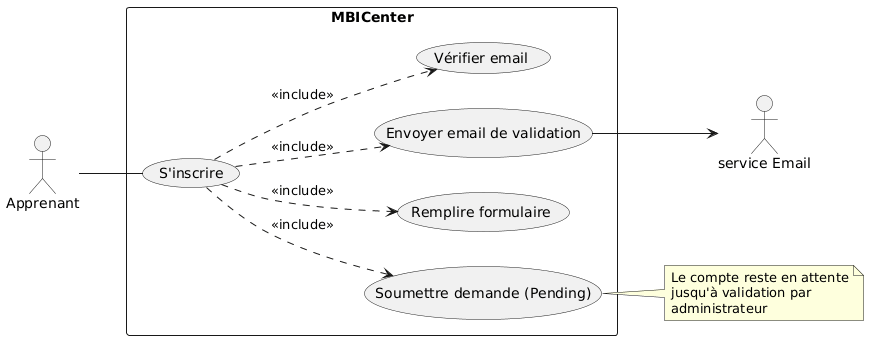
\includegraphics[width=1\textwidth]{project/images/abc.png}
    \caption{Diagramme de cas d’utilisation - Inscription}
    \label{fig:usecase}
    
\end{figure}
Le tableau \ref{tab:inscription_email} présente la description textuelle du cas d’utilisation « s’inscrire ».
\vspace{0.3cm} % petit espace avant le tableau

\small % optionnel : réduit légèrement la taille du texte du tableau
\begin{longtable}{|l|p{12cm}|}

\caption{Cas d’utilisation – Inscription et Vérification Email}
\label{tab:inscription_email} \\
\hline
\textbf{Élément} & \textbf{Description} \\
\hline
\endfirsthead
\hline
\textbf{Élément} & \textbf{Description} \\
\hline
\endhead

Cas d’utilisation & 
\begin{itemize}[leftmargin=*]
    \item inscription
\end{itemize} \\
\hline
Acteur & 
\begin{itemize}[leftmargin=*]
    \item apprenant
\end{itemize} \\
\hline
Préconditions & 
\begin{itemize}[leftmargin=*]
    \item L’utilisateur ne possède pas de compte
    \item L’utilisateur a accès à son email
\end{itemize} \\
\hline
Scénario de base & 
\textbf{Scénario 1 : Inscription} \\
& L’utilisateur saisit ses informations (nom, email, téléphone, mot de passe, confirmation, programme). \\
& Le système vérifie que tous les champs obligatoires sont remplis. \\
& Le système valide la conformité du mot de passe et sa correspondance avec la confirmation. \\
& Le système vérifie que l'email n'existe pas déjà dans la base de données. \\
& Le système chiffre le mot de passe et enregistre les données avec statut \textit{Non vérifié}. \\
& Le système envoie un email de vérification contenant un lien. \\

\hline
\vspace{0.3cm}
& \textbf{Scénario 2 : Vérification Email} \\
& -L’utilisateur clique sur le lien reçu. \\
& -Le système vérifie la validité du lien et l’existence de l’utilisateur. \\
& -Le système met à jour le statut vers \textit{En attente (Pending)}. \\
& -Le système affiche un message indiquant que l’inscription est réussie et en attente de validation par l’administrateur. \\
& -Le système envoie un email de confirmation à l’utilisateur. \\
\hline
Scénarios alternatifs & 
\textbf{Scénario 1: Inscription} \\
& \textbf{1.1 Email déjà utilisé:} Si l’email a déjà été enregistré, un message d’erreur pertinent s’affiche et l’utilisateur doit saisir un autre email. \\
& \textbf{1.2 Champs obligatoires vides:} Si un ou plusieurs champs requis ne sont pas remplis, un message d’erreur pertinent s’affiche et l’utilisateur doit compléter tous les champs. \\
& \textbf{1.3 Mot de passe non conforme:} Si le mot de passe ne respecte pas les règles (longueur minimale, caractères spéciaux…), un message d’erreur pertinent s’affiche et l’utilisateur doit corriger le mot de passe. \\
& \textbf{1.4 Confirmation du mot de passe incorrecte:} Si le mot de passe et sa confirmation ne correspondent pas, un message d’erreur pertinent s’affiche et l’utilisateur doit corriger la confirmation du mot de passe. \\
& \textbf{Scénario 2: Vérification Email} \\
& 2.1 Lien invalide ou expiré: Si le lien  de vérification est incorrect ou expiré, un message d’erreur pertinent s’affiche et l’utilisateur peut réessayer ou demander un nouveau lien. \\
\hline
Post-condition & 
\begin{itemize}
    \item L’utilisateur est enregistré dans le système.
    \item Le compte est en statut \textit{En attente de validation}.
    \item Un email de notification est envoyé.
\end{itemize} \\
\hline
\end{longtable}
\vspace{0.2cm}


\noindent\textbf{Amélioration du cas d’utilisation « authentification »:}

\noindent Une fois les comptes créés et pour les apprenants, leurs demandes d’inscription validées par l’administrateur, les utilisateurs peuvent accéder à la plateforme via la procédure d’authentification.
La figure \ref{fig:usecase_login} présente le diagramme de cas d’utilisation illustrant le processus de connexion.
\begin{figure}[H]
    \centering
    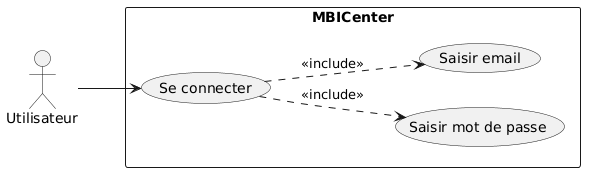
\includegraphics[width=0.7\textwidth]{project/images/RP2n3e9038Pt4jwXOOS4sGmXH2S79yC3D4V59iUTkIkJyTszYeD4r__x-ZTj7mM3BBFDipopT1KG3u6dcy38WOomTuhGY0ym25kEABG43VDC3NIJ9IZEXzEHd50euA48O8baC2Pq8J3UkUGgnGZ3iOQjWHmvmEpJMe8xHWrNS_TFf1dPVeGc2Uj2hQsgJeTW3stBpjXbfAxRmkONlYkUsl.png}
    \caption{Diagramme de cas d'utilisation "authentification"}
    \label{fig:usecase_login}
\end{figure}

\noindent Le tableau \ref{tab:authentification} présente la description textuelle du cas d’utilisation «Authentification».
\vspace{0.3cm} % petit espace avant le tableau

\small % optionnel : réduit légèrement la taille du texte du tableau
\begin{longtable}{|l|p{12cm}|}
\caption{Cas d’utilisation –Authentification} \label{tab:authentification} \\
\hline
\textbf{Élément} & \textbf{Description} \\
\hline
\endfirsthead
\hline
\textbf{Élément} & \textbf{Description} \\
\hline
\endhead

Cas d’utilisation & 
\begin{itemize}
    \item Authentification 
\end{itemize} \\
\hline
Acteur & 
\begin{itemize}
    \item Utilisateur
\end{itemize} \\
\hline
Préconditions & 
\begin{itemize}
    \item L'utilisateur possède un compte vérifié et approuvé dans le système

\end{itemize} \\
\hline
Scénario de base & 
1. L’utilisateur saisit  l'email  et le mot de passe \\
& 2. Le système vérifie que les champs ne sont pas vides \\
& 3. Le système vérifie que l’email existe dans la base de données\\
& 4. Le système compare le mot de passe saisi avec le mot de passe hashé\\
& 5.Le système vérifie le statut du compte  \\
& 6. Le système génère un JWT contenant (id,email,role)\\
& 7. Le token est stocké (Cookie sécurisé ou localStorage)\\
& 8. Le système redirige l’utilisateur vers son espace selon son rôle\\
\hline
Scénarios alternatifs & 
\textbf{Champs vides :}
 Le système affiche un message demandant de remplir tous les champs \\
& \textbf{Email inexistant :} Le système affiche un message d’erreur et refuse l’authentification \\
& \textbf{Mot de passe incorrect :} Le système affiche un message d’erreur et permet une nouvelle tentative \\
& \textbf{Compte non autorisé :} Le système bloque l’accès et affiche un message indiquant que le compte n’est pas autorisé \\
\hline
Post-condition & 
\begin{itemize}[leftmargin=*]
    \item Authentification réussie
    \item JWT généré
    \item Accès au dashboard selon le rôle
\end{itemize} \\
\hline
\end{longtable}


\noindent \textbf{Amélioration du cas d'utilisation « modification du mot de passe » :}

\noindent La fonctionnalité de récupération de mot de passe est essentielle pour permettre aux utilisateurs de réinitialiser leur mot de passe en cas d’oubli.
Elle comprend la soumission d’une demande de réinitialisation, la réception d’un lien de réinitialisation envoyé par email, l’accès à ce lien sécurisé, ainsi que la définition d’un nouveau mot de passe.

\noindent La figure \ref{fig:usecase_password_modification} présente le diagramme de cas d’utilisation expliquant le fonctionnement de la modification du mot de passe.
 \begin{figure}[H]
    \centering
    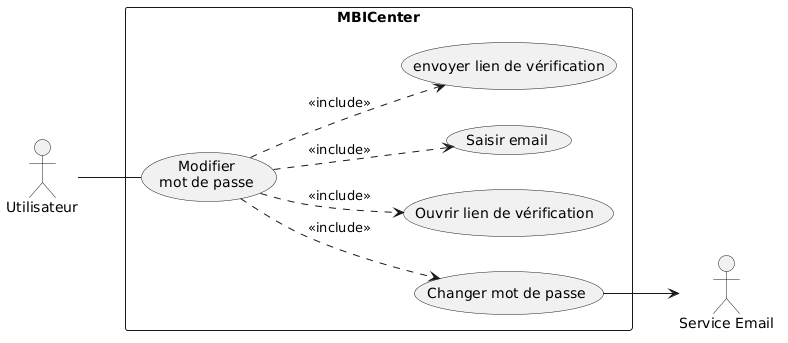
\includegraphics[width=1\textwidth]{project/images/ddcsc.png}
    \caption{Diagramme de cas d'utilisation "modification du mot de passe"}
    \label{fig:usecase_password_modification}
\end{figure}
\noindent Le tableau \ref{tab:password_modification} présente la description textuelle du cas d’utilisation «modification du mot de passe».

\begin{longtable}{|l|p{12cm}|}
\caption{cas d'utilisation-modification du mot de passe}
\label{tab:password_modification} \\
\hline
\textbf{Élément} & \textbf{Description} \\
\hline
\endfirsthead
\hline
\textbf{Élément} & \textbf{Description} \\
\hline
\endhead
Cas d’utilisation & Mot de passe oublié (Forgot Password) \\
\hline
Acteur & Utilisateur \\
\hline

Précondition & 
\begin{itemize}[leftmargin=*]
    \item L’utilisateur a oublié son mot de passe
    \item L’utilisateur possède un compte dans le système
\end{itemize} \\
\hline
Scénario principal & 
\textbf{ Scénario 1: Demande de réinitialisation}
\begin{enumerate}[leftmargin=*]
    \item L’utilisateur clique sur « Mot de passe oublié »
    \item Il saisit son adresse email
    \item Le système vérifie la validité de l’email
    \item Le système vérifie l’existence de l’email en base
    \item Le système envoie un lien de réinitialisation unique et temporaire
    \item Le système affiche un message de confirmation
\end{enumerate}

\textbf{Scénario 2: Réinitialisation du mot de passe}
\begin{enumerate}[leftmargin=*]
    \item L’utilisateur ouvre le lien reçu par email
    \item Il saisit le nouveau mot de passe et sa confirmation
    \item Le système vérifie que les champs sont remplis
    \item Le système vérifie que les mots de passe sont identiques
    \item Le système vérifie la validité du lien (token non expiré)
    \item Le système met à jour le mot de passe (hash)
    \item Le système affiche un message de succès et redirige vers login
\end{enumerate}
\\
\hline
Scénarios alternatifs & 
\begin{itemize}[leftmargin=*]
    \item \textbf{Email invalide ou vide :} le système affiche un message d’erreur et bloque l’envoi
    \item \textbf{Email inexistant :} affichage d’un message générique pour des raisons de sécurité
    \item \textbf{Mots de passe non identiques :} le système rejette la demande
    \item \textbf{Lien expiré ou déjà utilisé :} le système affiche une erreur et demande une nouvelle réinitialisation
\end{itemize}
\\
\hline

Postcondition & 
\begin{itemize}[leftmargin=*]
    \item Un lien de réinitialisation est généré
    \item Un email est envoyé à l’utilisateur
    \item L’utilisateur accède au formulaire de réinitialisation
    \item Le mot de passe est mis à jour dans la base de données
    \item L’utilisateur peut se reconnecter avec le nouveau mot de passe
\end{itemize}
\\
\hline
\end{longtable}

\subsection{Conception}
La phase de conception modélise techniquement le fonctionnement de l'authentification à l'aide de diagrammes de séquence. Ils illustrent chronologiquement les interactions entre l'utilisateur et le système pour garantir la sécurité des flux, depuis l'inscription de l'apprenant jusqu'à sa validation finale par l'administration.
\vspace{0.3cm}

\noindent\textbf{Diagramme de séquence : Inscription de l'apprenant}

\noindent Ce diagramme illustre le processus de création d'un nouveau compte sur la plateforme. L'utilisateur fournit ses donnés personnelles. La figure \ref{cap:inscription_apprenant} presente comment le système procède d'abord à une vérification du format des données et l'unicité de l'email. Une fois validé, le mot de passe est haché et le compte est créé avec un statut "non vérifié". Un lien de confirmation est alors envoyé par email à l'utilisateur pour confirmer l'identité de l'apprenant.

\vspace{0.3cm}
\noindent \textbf{Diagramme de séquence : Vérification de l'adresse email}

\noindent Ce diagramme démontre la validation de l'email,comme il est représenté dans la Figure \ref{cap:usecase_seq_verif}, faisant passer le compte du statut "non vérifié" à "en attente". En cliquant sur le lien reçu, l'apprenant transmet un code de sécurité que le système vérifie (intégrité et validité). Une fois l'email confirmé, le profil est prêt pour l'étape finale : l'examen et la validation manuelle par l'administrateur.

\vspace{0.3cm}
\noindent\textbf{Diagramme de séquence : Login}

\noindent Le processus d’authentification est  détaillé en deux scénarios spécifiques : le login de l’apprenant et celui du responsable, afin de distinguer les différents parcours d’accès selon le rôle de l’utilisateur.

\newpage
\thispagestyle{empty}

\begin{figure}[H]
\centering

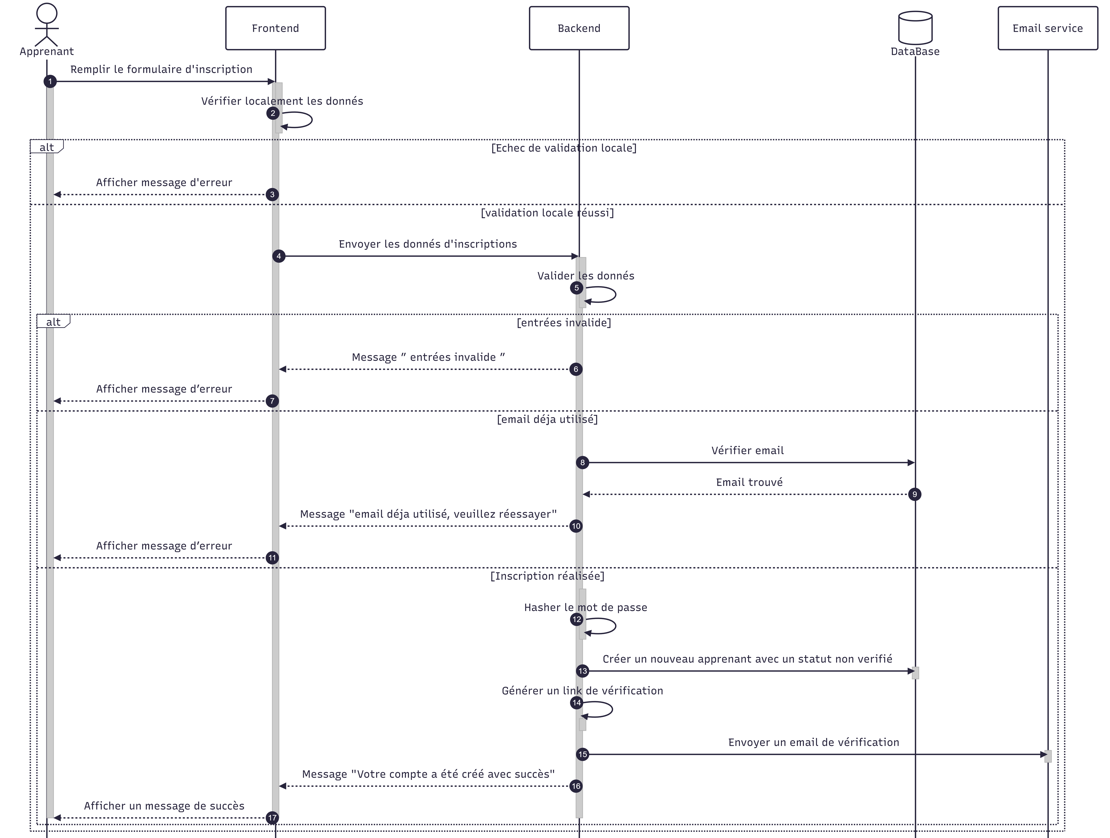
\includegraphics[height=0.45\textheight,keepaspectratio]{project/images/inscds.png}

\caption{Diagramme de séquence <<Inscription de l'apprenant>>}
\label{cap:inscription_apprenant}

\end{figure}

\begin{figure}[H]
  \centering
    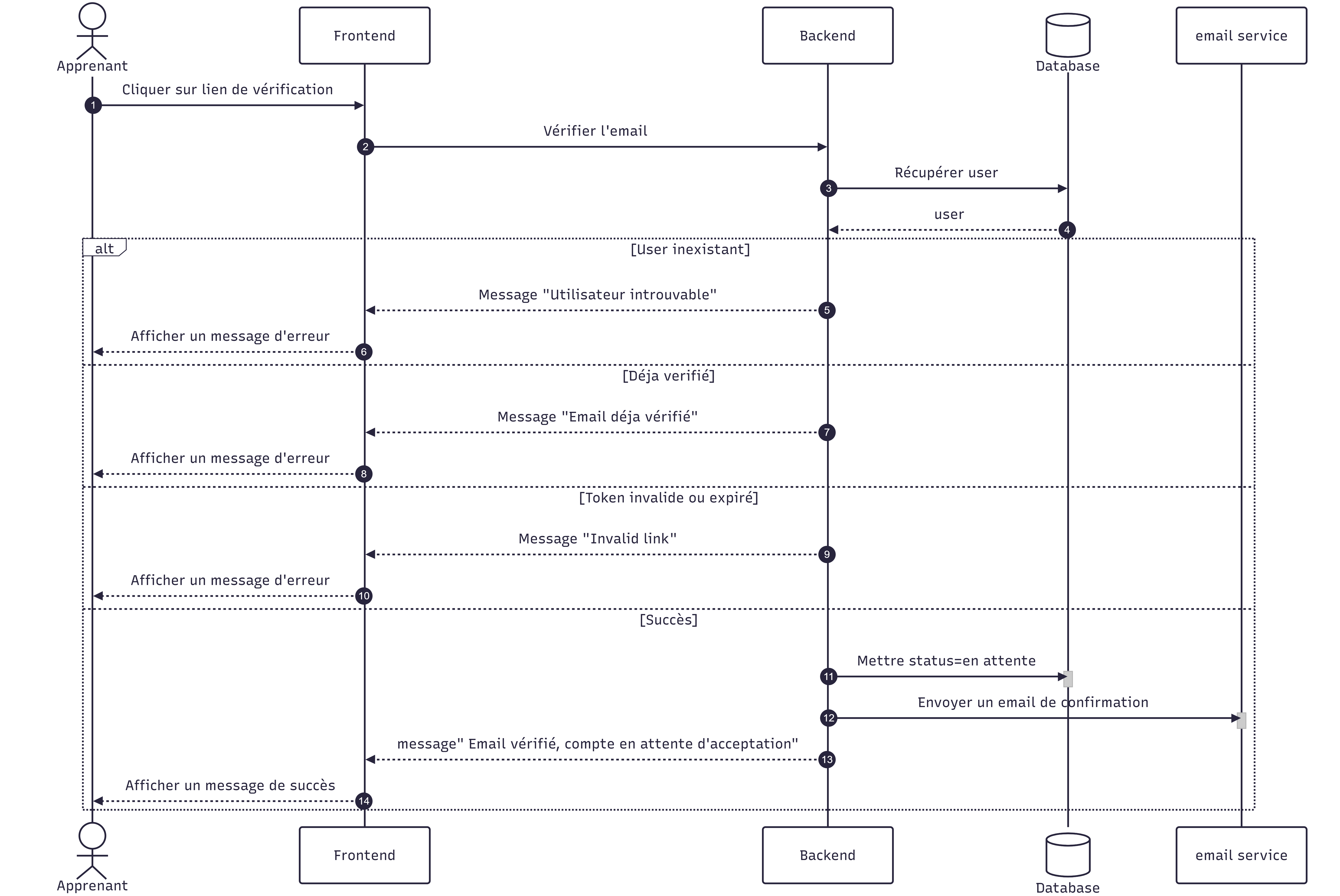
\includegraphics[width=\textwidth,height=0.9\textheight,keepaspectratio]{project/images/Verify-mail.png}
  \caption{Diagramme de séquence <<Vérification de l'adresse email>> }
  \label{cap:usecase_seq_verif}
\end{figure}


\vspace{0.3cm}

\noindent \textbf{Diagramme de séquence: Login -Apprenant}

\noindent le diagramme décrit la procédure de connexion sécurisée pour le profil apprenant, qui est schématisé dans la Figure \ref{cap:Diagramme de séquence <<Login - Apprenant>>}.
\vspace{0.3cm}

\begin{figure}[H]
  \centering
    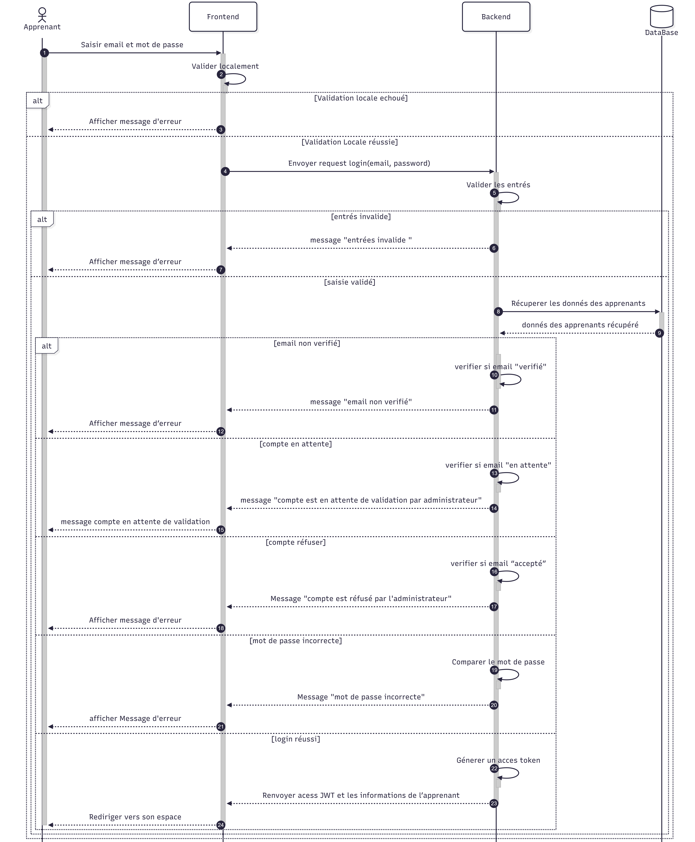
\includegraphics[scale=0.9]{project/images/loginds.png}
  \caption{Diagramme de séquence <<Login - Apprenant>> }
  \label{cap:Diagramme de séquence <<Login - Apprenant>>}
\end{figure}
\newpage
\noindent \textbf{Diagramme de séquence : Login -Responsables et Administrateurs}

\noindent Le diagramme exposé dans la Figure \ref{cap:Diagramme de séquence <<Login -Responsables et Administrateurs>>}, présente le flux d’authentification pour les profils administratifs, tels que le Directeur, le Responsable pédagogique , Responsable financier ou l’Administrateur. Bien que ces utilisateurs possèdent des niveaux d’accès différents, leurs étapes de connexion sont identiques, ce qui justifie la conception d’un diagramme unifié.



\begin{figure}[H]
  \centering
    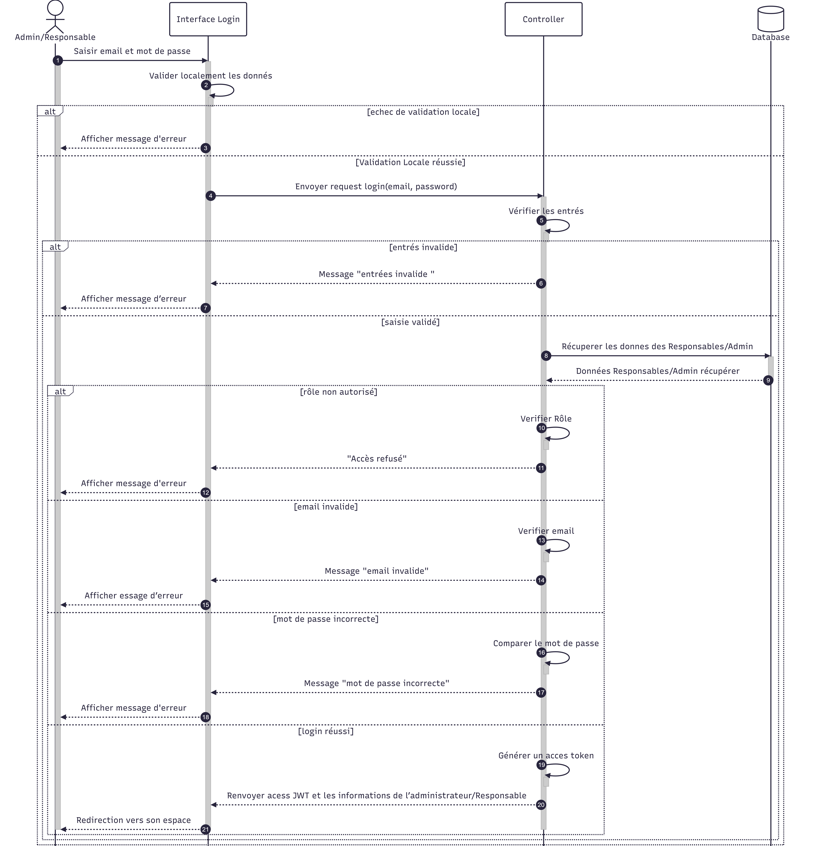
\includegraphics[scale=0.8]{project/images/LoginResds.png}
  \caption{Diagramme de séquence <<Login -Responsables et Administrateurs>> }
  \label{cap:Diagramme de séquence <<Login -Responsables et Administrateurs>>}
  \centering
\end{figure}

\newpage
\noindent\textbf{Diagramme de séquence: Mot de passe oublié}

\noindent Ce diagramme modelise la demande de récupération de compte. Après avoir vérifié l'existence de l'utilisateur, le système lui envoie un lien de réinitialisation temporaire par email comme il est représenter dans la Figure \ref{cap:Diagramme de séquence <<Mot de passe oublié>>}. Ce mécanisme sécurisé garantit que seul le propriétaire légitime de la boîte mail peut initier la modification de son mot de passe.
\vspace{0.5cm}
\begin{center}
  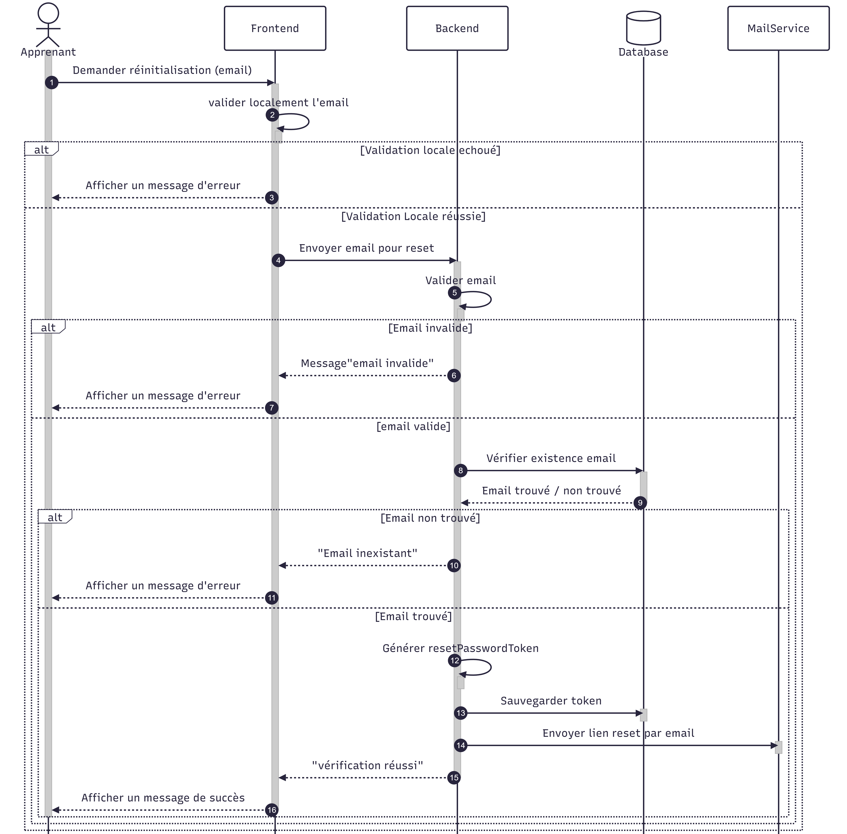
\includegraphics[width=1.1\textwidth,keepaspectratio]{project/images/forgetpassds.png}
  \captionof{figure}{Diagramme de séquence <<Mot de passe oublié>>}
  \label{cap:Diagramme de séquence <<Mot de passe oublié>>}
\end{center}
\newpage
\noindent\textbf{Diagramme de séquence : Vérification de lien de réinitialisation}

Ce diagramme décrit la validation automatique du lien envoyé par email. Avant d'autoriser tout changement, le système vérifie si le lien utilisé est toujours fonctionnel. Cela permet de bloquer la procédure si le lien a expiré, évitant ainsi à l'utilisateur de perdre du temps avec un lien expiré comme illustré dans la Figure \ref{cap:usecase_seq_linkReset}.

\begin{figure}[H]
  \centering
    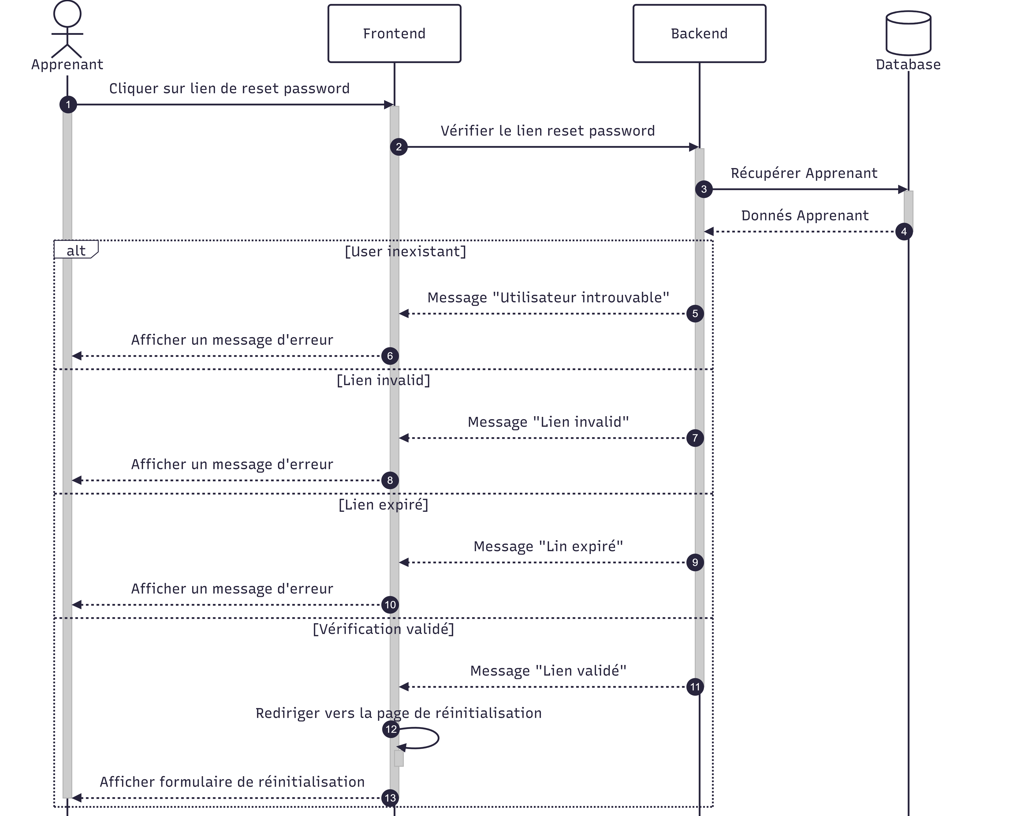
\includegraphics[width=1.1\textwidth,height=0.9\textheight,keepaspectratio]{project/images/linkressds.png}
  \caption{Diagramme de séquence <<Vérification du lien de réinitialisation>> }
  \label{cap:usecase_seq_linkReset}
\end{figure}

\vspace{0.3cm}

\noindent\textbf{Diagramme de séquence : Réinitialisation du mot de passe}

\noindent Ce dernier diagramme schématisé dans la Figure \ref{cap:Diagramme de séquence:<<Réinitialisation du mot de passe>>} présente la mise à jour finale du mot de passe. L’utilisateur saisit ses nouvelles informations, qui sont envoyées de manière  sécurisée au système. Après une vérification finale de la demande, le système sécurise le nouveau mot de passe et l’enregistre dans la base de données.
\newpage
\begin{figure}[H]
  \centering
    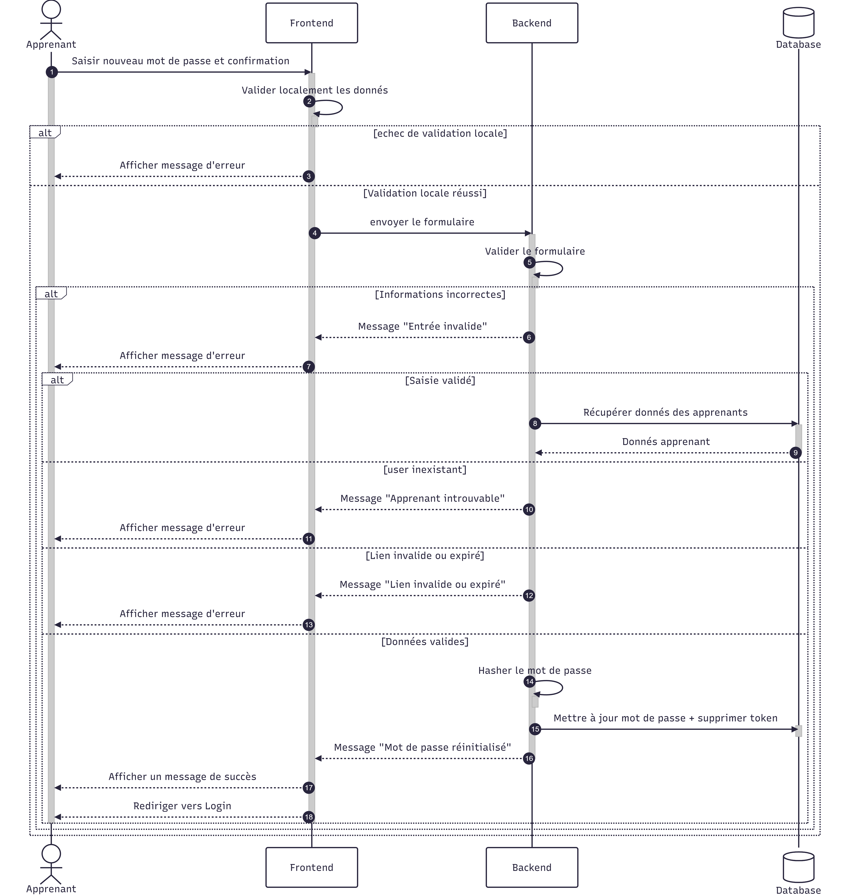
\includegraphics[width=1.1\textwidth,height=1\textheight,keepaspectratio]{project/images/newpassds.png}
  \caption{Diagramme de séquence <<Réinitialisation du mot de passe>> }
  \label{cap:Diagramme de séquence:<<Réinitialisation du mot de passe>>}
\end{figure}




\newpage
\subsection{Réalisation}
Cette section présente les interfaces de l'authentification. Nous allons détailler les différents modules en mettant l’accent sur l’expérience utilisateur et les fonctionnalités implémentées.

\vspace{0.3cm}
\noindent\textbf{Interface d'inscription}

\noindent La première étape pour l'apprenant est de renseigner ses informations de base via une interface intuitive. Comme l'illustre la Figure \ref{cap:Interface d'inscription:standard}, le formulaire comprend des champs obligatoires avec une aide à la saisie pour guider l'apprenant. La figure \ref{cap:Interface d'inscription:champs-vide} montre comment l'interface réagit lorsque les données ne respectent pas le format attendu (par exemple, un mot de passe trop simple ou un email mal formé). Si un utilisateur tente de s'inscrire avec un email déjà existant, une alerte spécifique est déclenchée comme le montre la figure \ref{cap:Interface d'inscription:champs-invalide}.

\begin{center}


\begin{minipage}{0.9\textwidth}
    \centering
    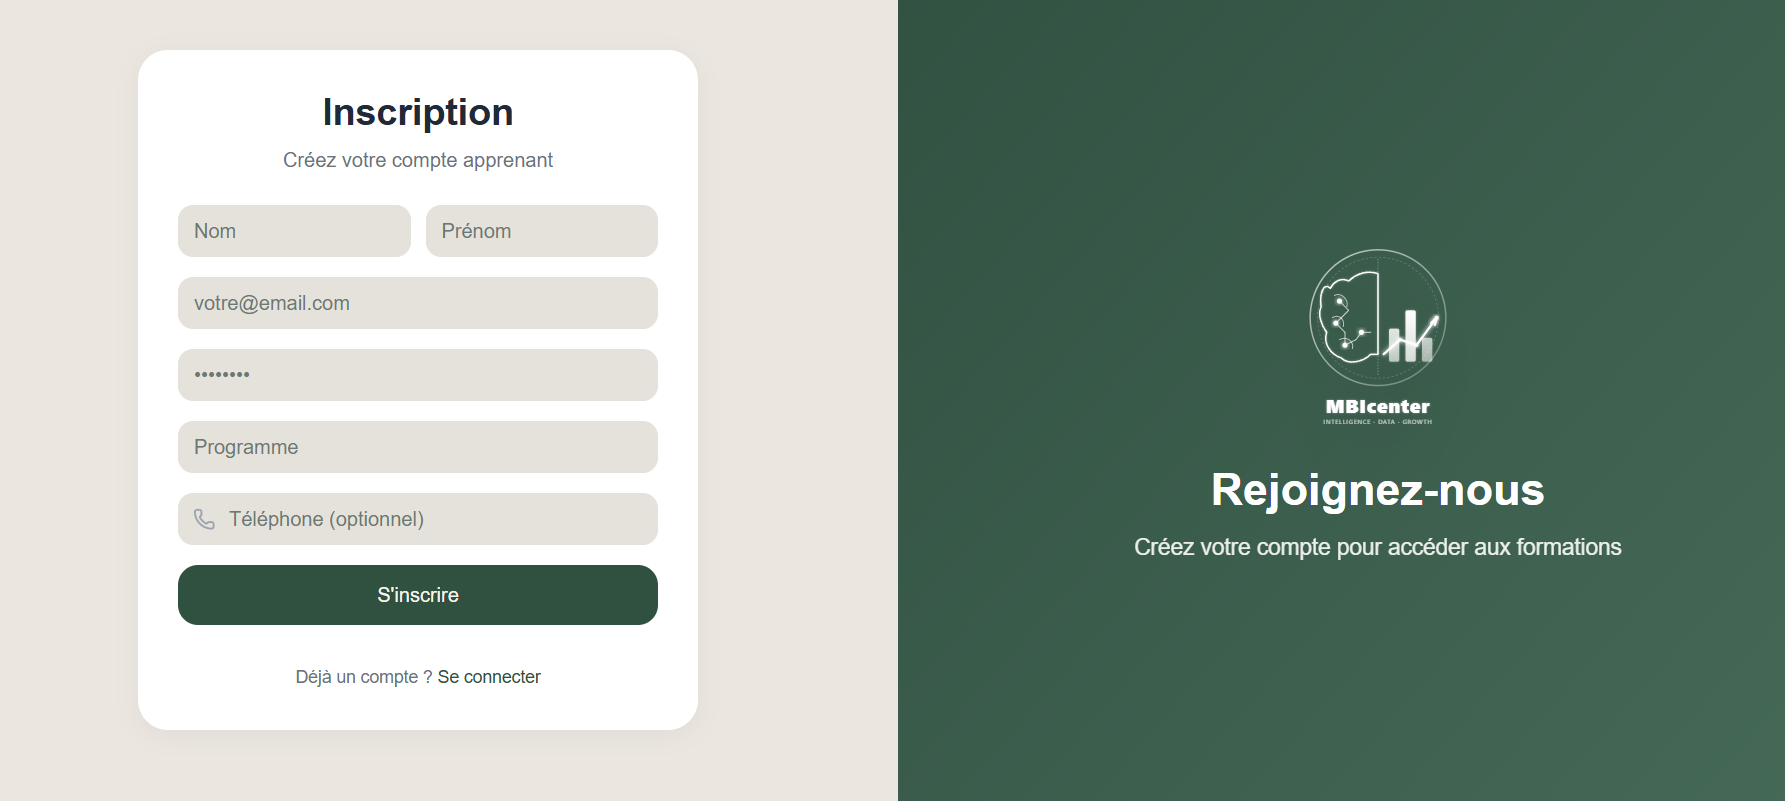
\includegraphics[width=1\linewidth]{project/images/register-cap.png}
    \captionof{figure}{Interface d'inscription : standard}
    \label{cap:Interface d'inscription:standard}
\end{minipage}

\begin{minipage}{0.45\textwidth}
    \centering
    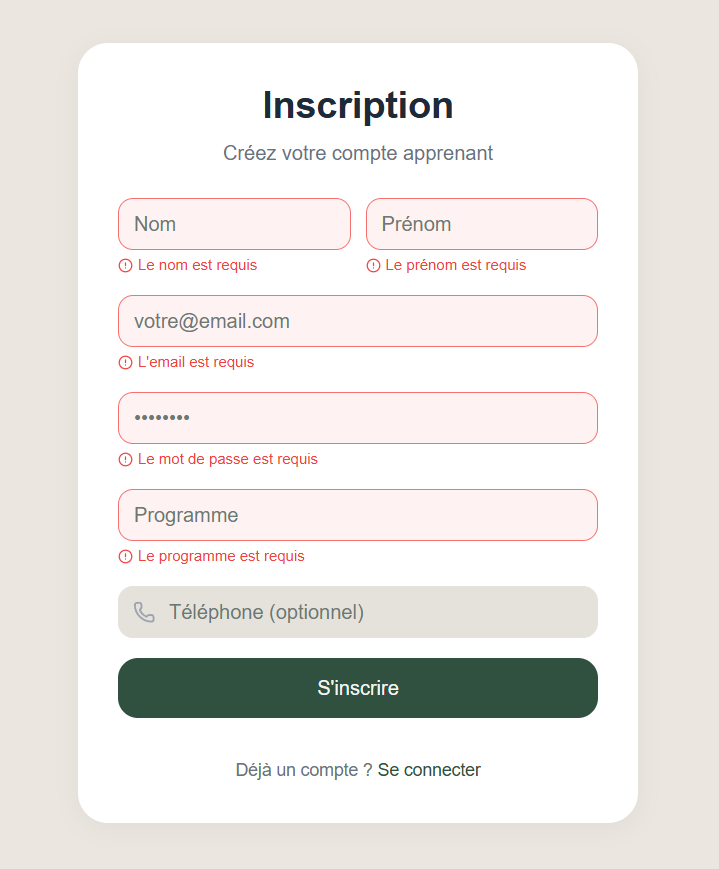
\includegraphics[width=0.9\linewidth]{project/images/register-empty.png}
    \captionof{figure}{Interface d'inscription : champs vides}
    \label{cap:Interface d'inscription:champs-vide}
\end{minipage}
\hfill
\begin{minipage}{0.45\textwidth}
    \centering
    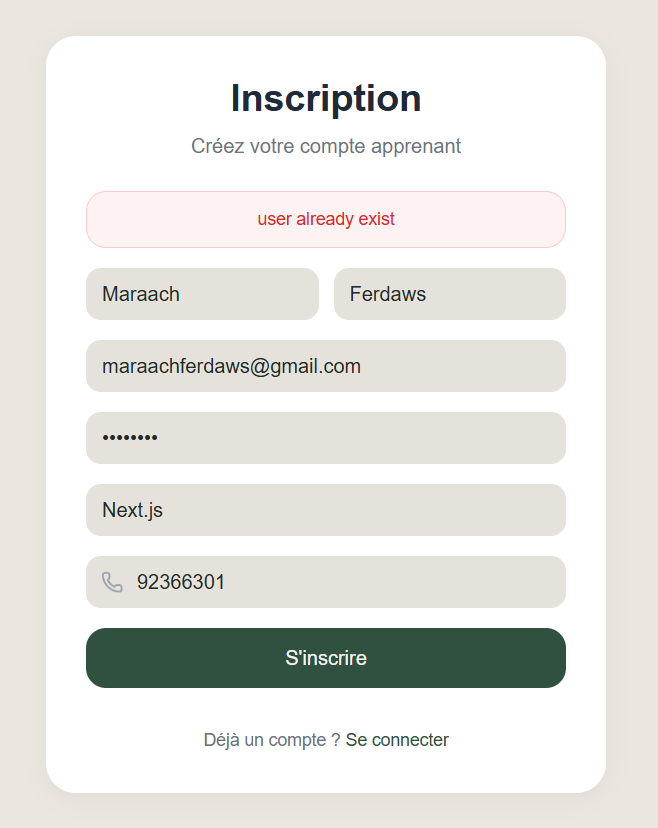
\includegraphics[width=0.9\linewidth]{project/images/register-invalid.png}
    \captionof{figure}{Interface d'inscription : champs invalides}
    \label{cap:Interface d'inscription:champs-invalide}
\end{minipage}

\vspace{0.4cm}



\end{center}

\FloatBarrier

\newpage
\noindent \textbf{Étape de la Vérification d'email}

\noindent L’interface illustrée en Figure \ref{cap:interface d'inscription: vérifier email} informe l'utilisateur qu'un lien de confirmation a été envoyé à son adresse mail pour valider son compte. À cette étape, la Figure \ref{cap:interface d'inscription: email de vérification}  présente le contenu du mail reçu par l'utilisateur, incluant un bouton sécurisé contenant un token d'activation. 

\noindent Dans le cas où l'utilisateur clique sur un lien déjà utilisé ou dont la durée de validité est dépassée, l’interface de la \ref{cap:interface d'inscription:lien non valide} s'affiche pour lui proposer de renvoyer un nouvel email de vérification.

\noindent Enfin, comme le montre la Figure \ref{cap:interface d'inscription:inscription vérifié}, une page de confirmation apparaît brièvement suite à une validation réussie, avant de rediriger automatiquement l'utilisateur vers la page de connexion.



\begin{center}
    \centering
    
    % الصف الأول
    \begin{minipage}{0.45\textwidth}
        \centering
        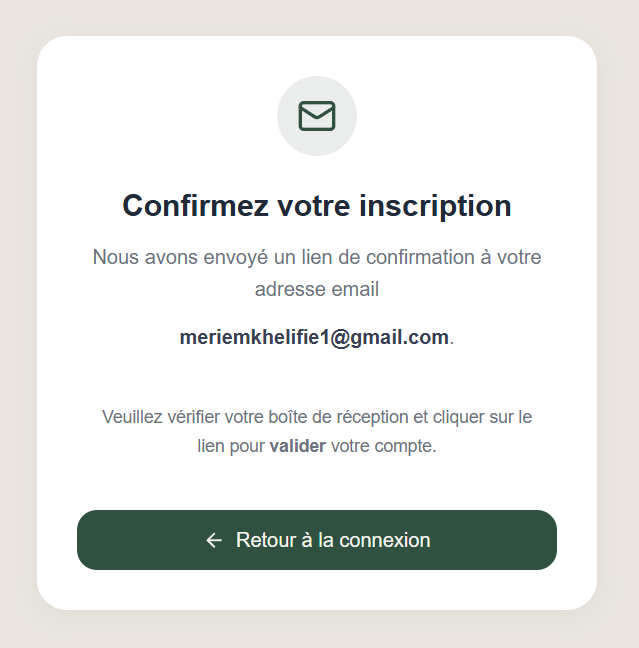
\includegraphics[width=1\linewidth]{project/images/confirme.png}
        \captionof{figure}{interface d'inscription : vérifier email}
        \label{cap:interface d'inscription: vérifier email}
    \end{minipage}
    \hfill
    \begin{minipage}{0.45\textwidth}
        \centering
        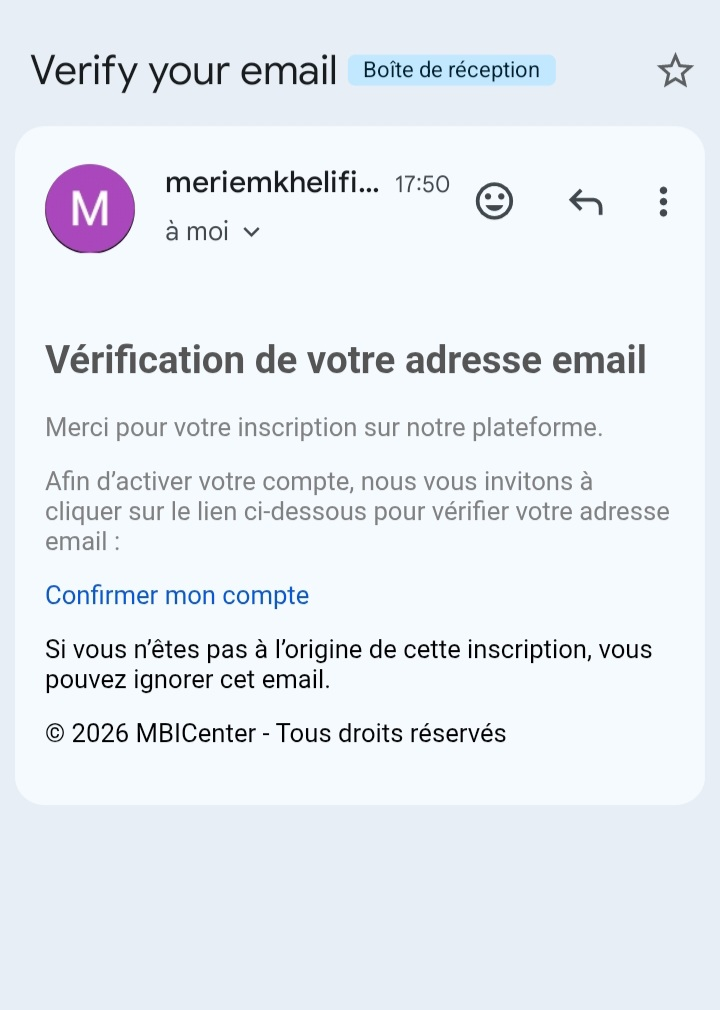
\includegraphics[width=0.8\linewidth]{project/images/email.verify.jpeg}
        \captionof{figure}{interface d'inscription : email de vérification}
        \label{cap:interface d'inscription: email de vérification}
    \end{minipage}
    
    \vspace{0.5cm}
    
    % الصف الثاني
    \begin{minipage}{0.45\textwidth}
        \centering
        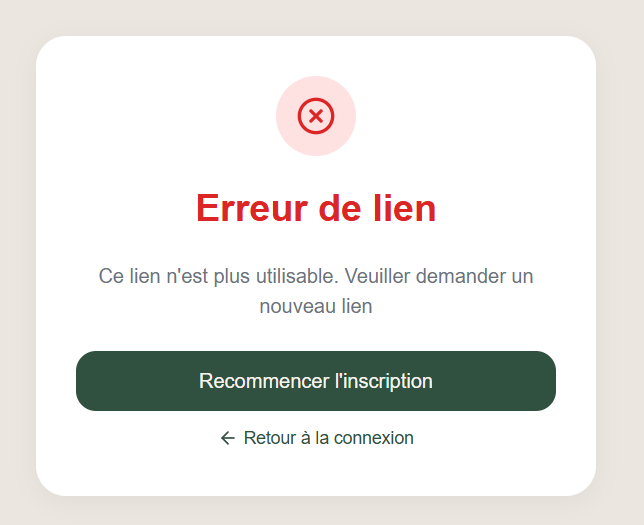
\includegraphics[width=1\linewidth]{project/images/lien-invalide.png}
        \captionof{figure}{interface d'inscription : lien non valide}
        \label{cap:interface d'inscription:lien non valide}
    \end{minipage}
    \hfill
    \begin{minipage}{0.45\textwidth}
        \centering
        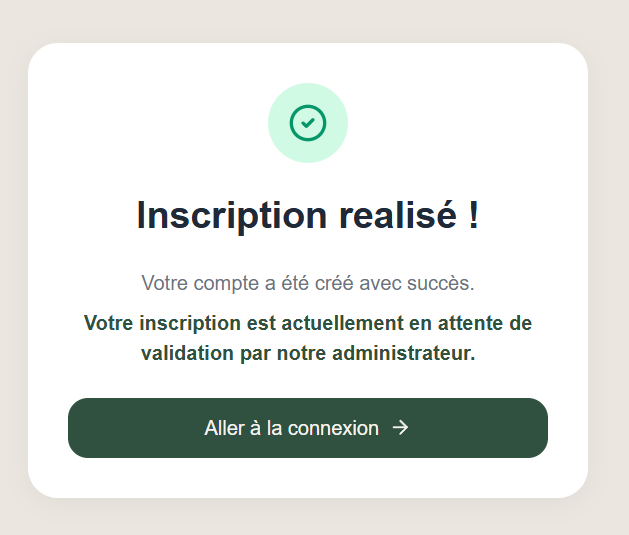
\includegraphics[width=0.8\linewidth]{project/images/validé.png}
        \captionof{figure}{interface d'inscription : inscription vérifié}
        \label{cap:interface d'inscription:inscription vérifié}
    \end{minipage}

\end{center}

\newpage
\noindent\textbf{Interface Login:}

\noindent L’interface de connexion dans la Figure \ref{fig:Interface login:état normale}  constitue le point d’entrée unique pour tous les utilisateurs. Afin de sécuriser l'accès, un message d’erreur s’affiche en cas d’identifiants incorrects comme la montre Figure \ref{cap:Interface login: données invalide}. Le système vérifie également le statut du compte : les profils en attente de validation illustré dans la Figure \ref{cap:Interface login:Apprenant ena attente d'acceptation} ou rejetés, représenté dans la Figure \ref{cap:Interface login:Apprenant-est-refusé} sont informés par des interfaces spécifiques. Par ailleurs, si le compte est désactivé, l’accès est refusé et un message d’erreur dédié est affiché, comme le montre la Figure \ref{cap:Interface login: Utilisateur désactivé}. Une fois l'authentification réussie, la plateforme redirige automatiquement l'utilisateur vers un espace selon son rôle.


\begin{figure}[H]
  \centering
    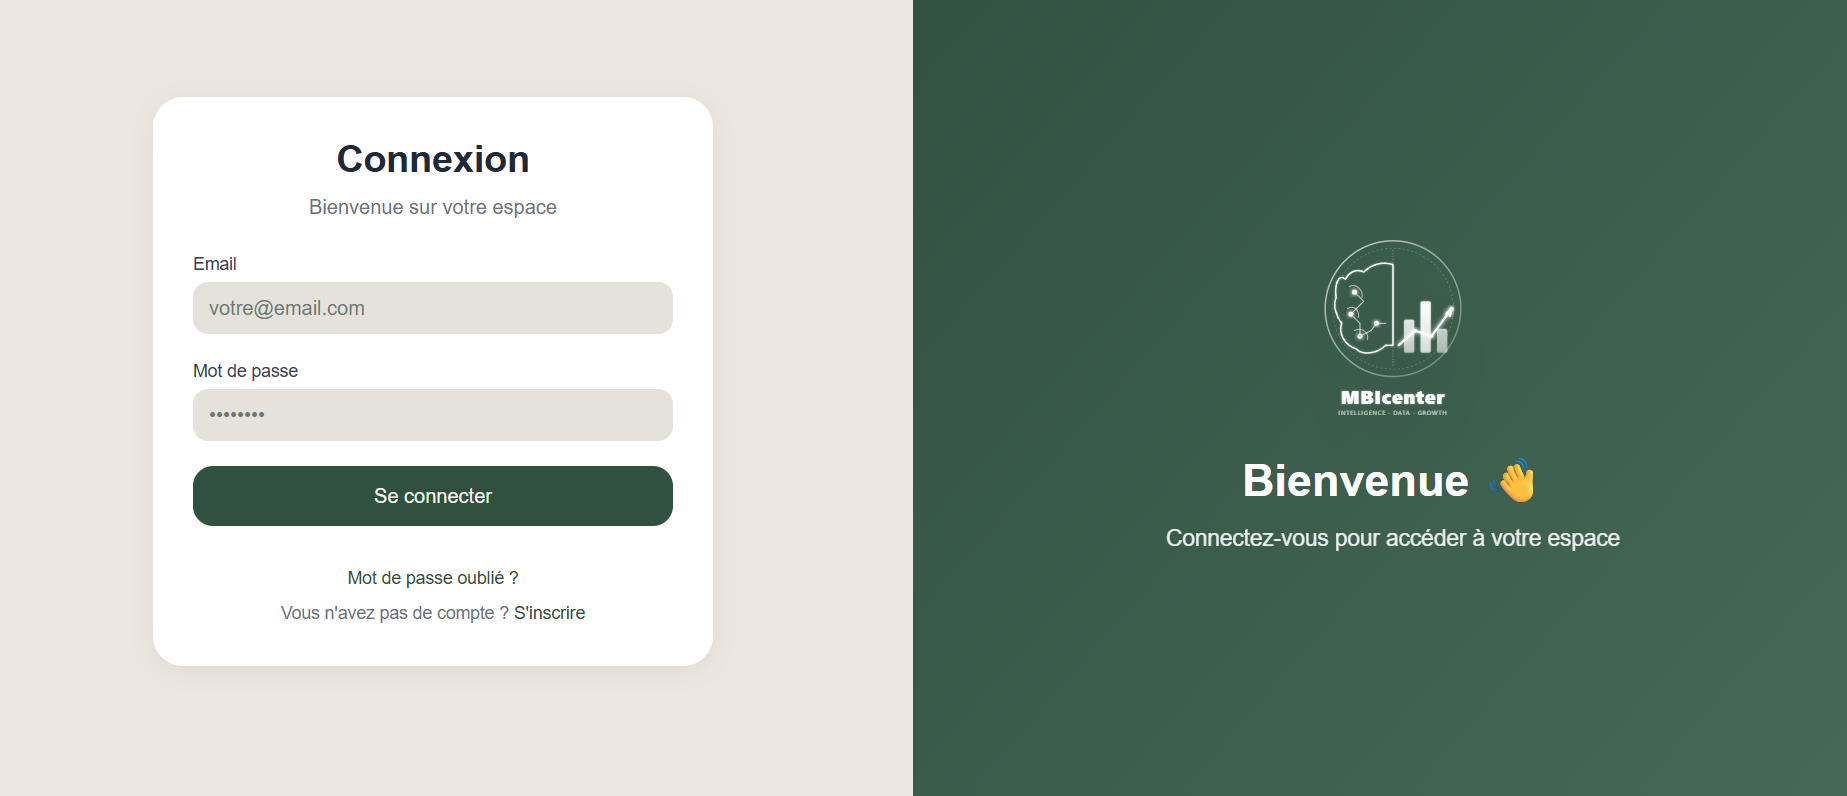
\includegraphics[width=1\linewidth]{project/images/login.png}
  \caption{ Interface login : état normale}
  \label{fig:Interface login:état normale}
\end{figure}

\begin{center}
    \centering
    
    % الصف الأول
    \begin{minipage}{0.45\textwidth}
        \centering
        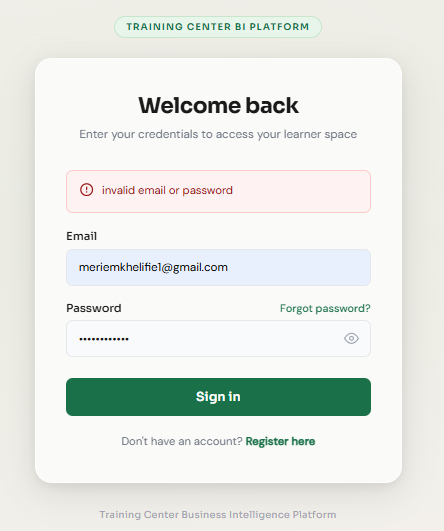
\includegraphics[width=0.9\linewidth]{project/images/Login-invalide.png}
        \captionof{figure}{Interface login : données invalide}
        \label{cap:Interface login: données invalide}
    \end{minipage}
    \hfill
    \begin{minipage}{0.5\textwidth}
        \centering
        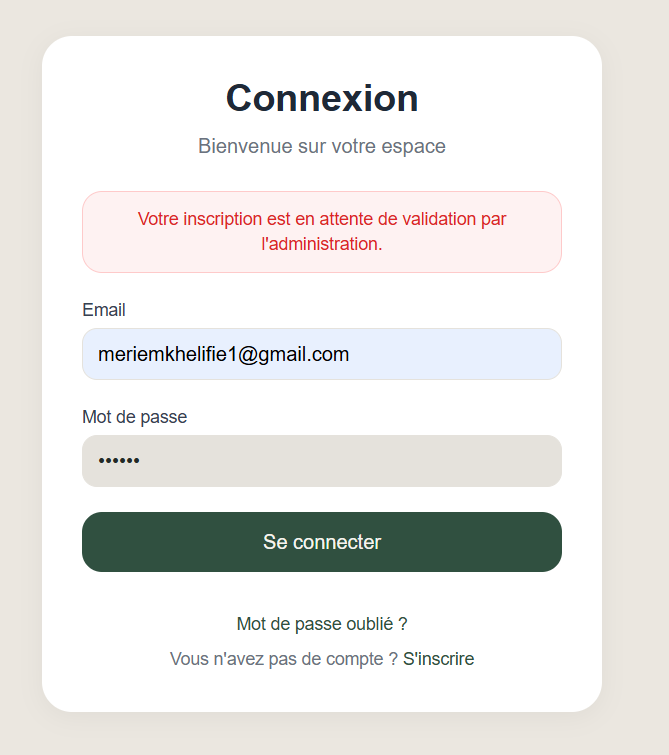
\includegraphics[width=0.79\linewidth]{project/images/en attente.png}
        \captionof{figure}{Interface login : Apprenant en attente d'acceptation}
        \label{cap:Interface login:Apprenant ena attente d'acceptation}
    \end{minipage}
\end{center}
    \vspace{0.5cm}
    % الصورة في الوسط
\begin{center}
    \centering  
    \begin{minipage}{0.45\textwidth}
        \centering
        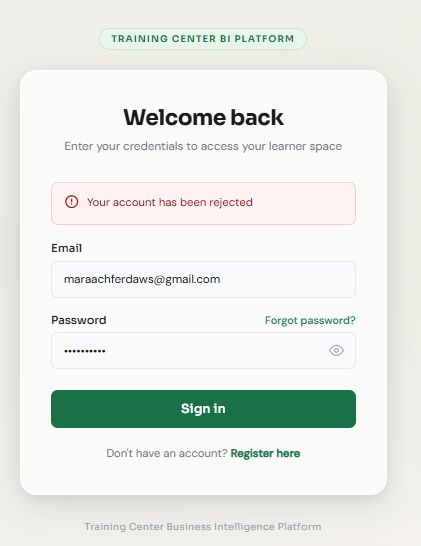
\includegraphics[width=0.9\linewidth]{project/images/rejected.png}
        \captionof{figure}{Interface login : Apprenant est refusé}
        \label{cap:Interface login:Apprenant-est-refusé}
    \end{minipage}
    \hfill
    \begin{minipage}{0.45\textwidth}
        \centering
        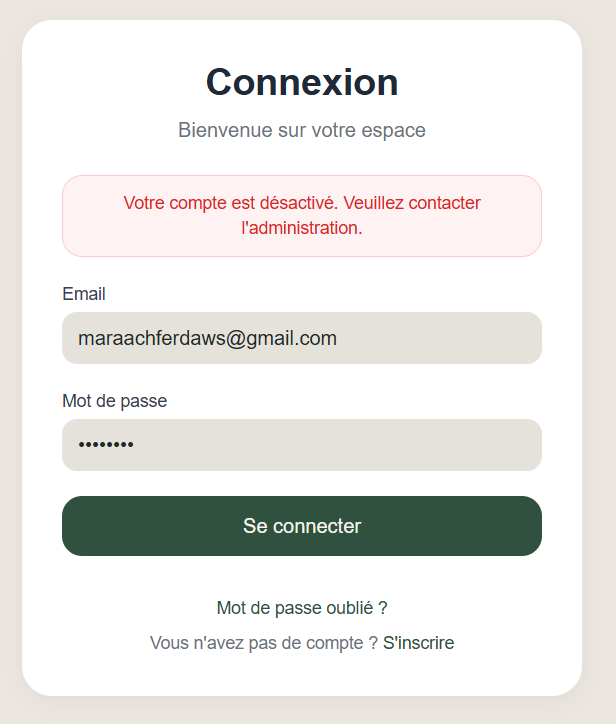
\includegraphics[width=0.9\linewidth]{project/images/compte-désactivé.png}
        \captionof{figure}{Interface login : Utilisateur désactivé}
        \label{cap:Interface login: Utilisateur désactivé}
    \end{minipage}
\end{center}







\noindent \textbf{Interface Réinitialisation du mot de passe:}

\noindent L’interface illustrée en Figure \ref{cap:R_mp} permet à l'utilisateur de saisir son adresse email pour initier la procédure.
Si l'adresse saisie ne correspond à aucun compte enregistré ou si le format est incorrect, l'interface de la Figure \ref{cap:F_F} s'affiche.

\vspace{0.8cm}

\begin{figure}[H]
  \centering
    \centering
        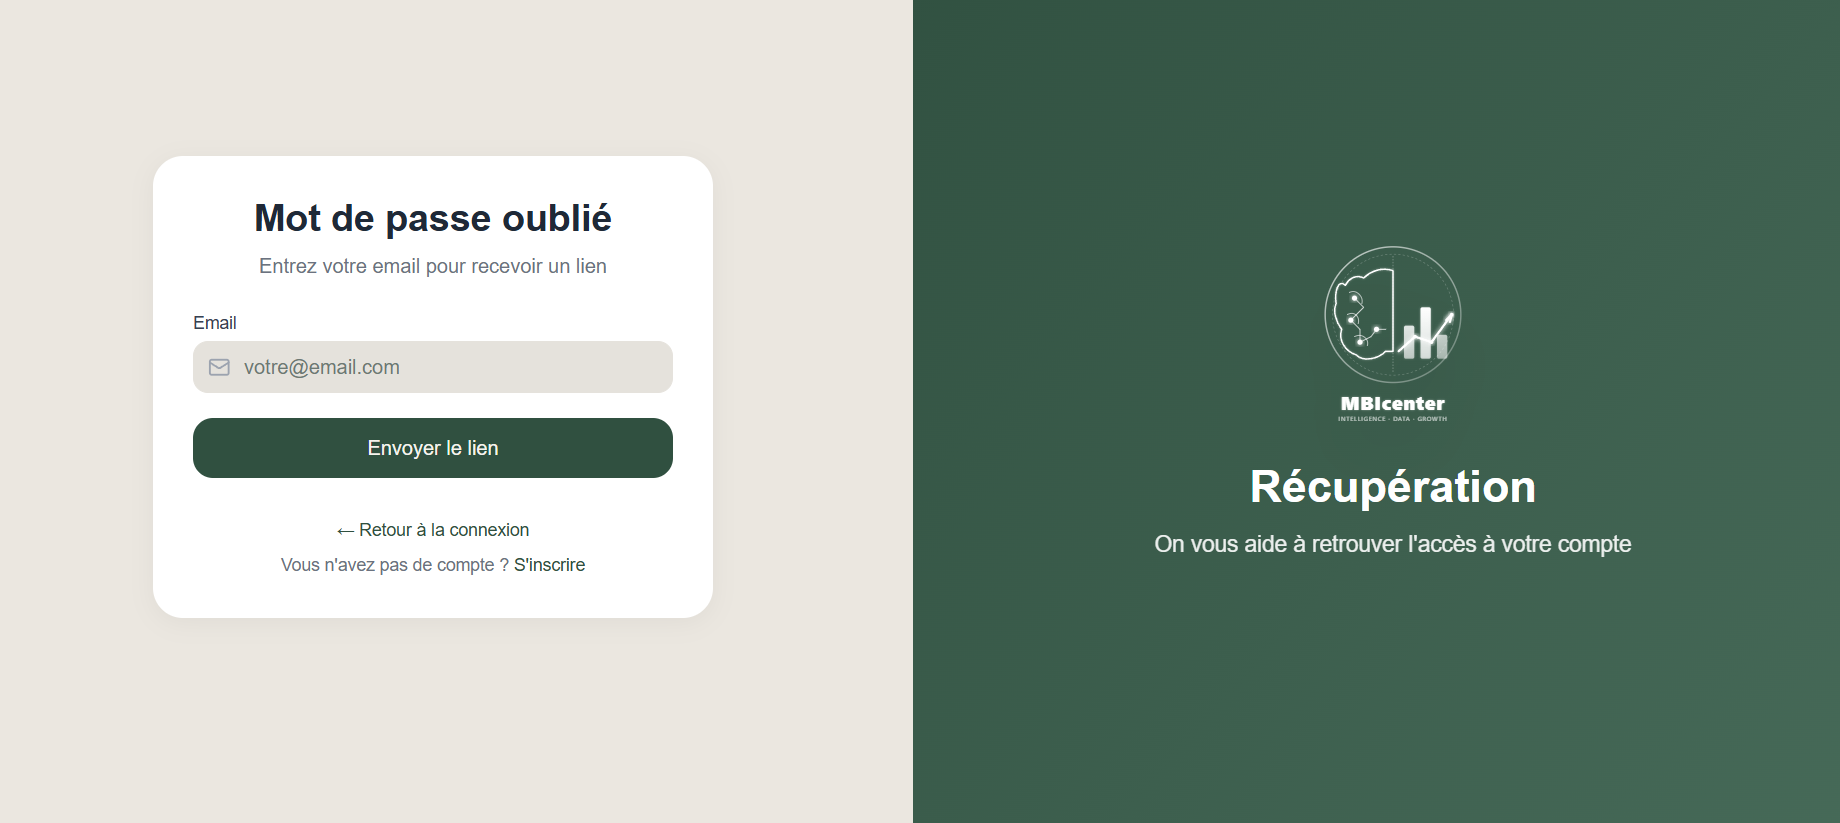
\includegraphics[width=\linewidth]{project/images/forgot-pass.png}
        \captionof{figure}{Interface de réinitialisation du mot de passe }
        \label{cap:R_mp}
\end{figure}


\begin{figure}[H]
    \centering
        \centering
        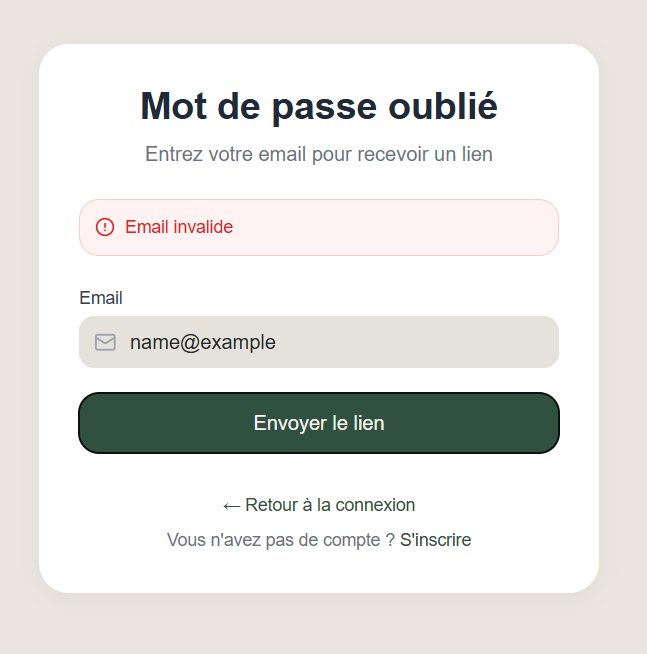
\includegraphics[width=0.5\linewidth]{project/images/pass-invalide.png}
        \captionof{figure}{Interface de réinitialisation : email invalide}
        \label{cap:F_F}
\end{figure}


\noindent \textbf{interface de lien de vérification :}

\noindent Une fois un email valide soumis comme le montre la figure \ref{cap:Interface réinitialisation: email }  , l'interface de la Figure \ref{cap:Interface de réinitialisation:email de réinitialisation} informe l'utilisateur qu'un lien de réinitialisation lui a été envoyé. Cette étape confirme la prise en compte de la demande par le serveur.

\noindent En accédant à ce lien, l’utilisateur est redirigé vers une interface dédiée à la réinitialisation du mot de passe, comme le montre la figure \ref{cap:Interface de réinitialisation:etat}, où il peut saisir un nouveau mot de passe.

\noindent Le lien envoyé par email a une durée de validité limitée. Si l'utilisateur clique sur un lien obsolète ou déjà utilisé, l'interface présentée en Figure \ref{cap:Interface de réinitialisation: lien invalide} apparaît, l'invitant à renouveler sa demande.

 \begin{center}
    \centering  
    \begin{minipage}{0.45\textwidth}
        \centering
        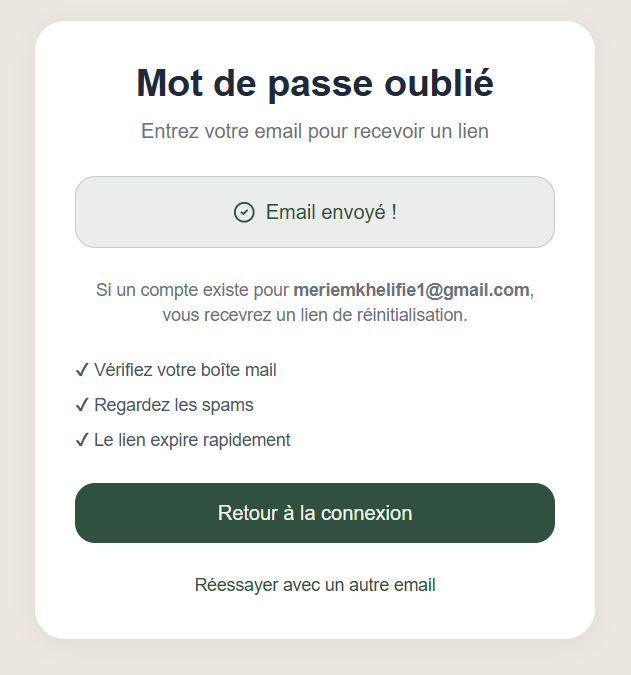
\includegraphics[width=0.9\linewidth]{project/images/pas-mail.png}
        \captionof{figure}{Interface de réinitialisation : email envoyé}
        \label{cap:Interface réinitialisation: email }
    \end{minipage}
    \hfill
    \begin{minipage}{0.45\textwidth}
        \centering
        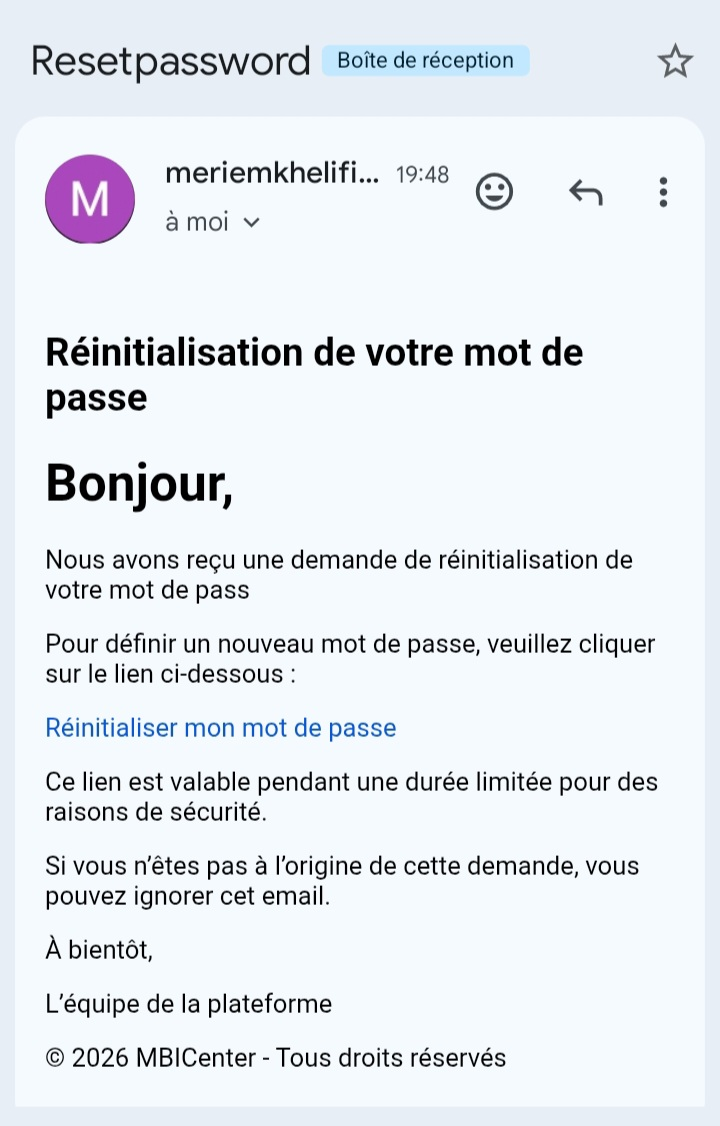
\includegraphics[scale=0.23]{project/images/email-reset.jpeg}
        \captionof{figure}{Interface de réinitialisation : email de réinitialisation}
        \label{cap:Interface de réinitialisation:email de réinitialisation}
    \end{minipage}
\end{center}

    
  
    
  
 \begin{center}   
    % الصف اللي لتحت (زوز صور)
    \begin{minipage}{0.45\textwidth}
        \centering
        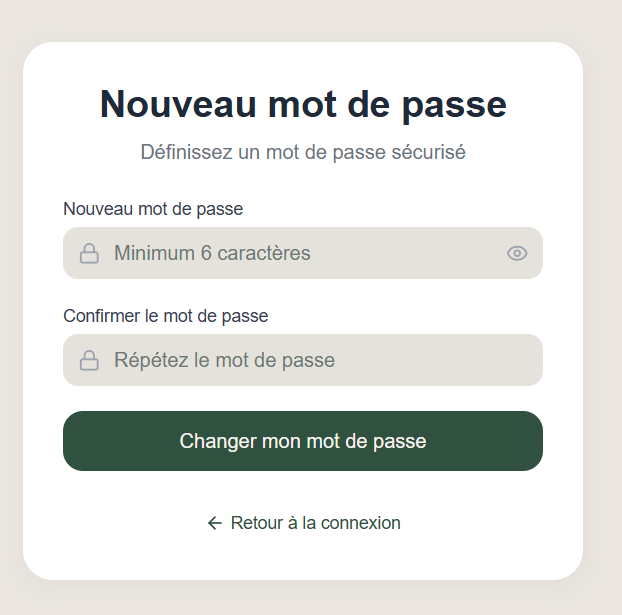
\includegraphics[width=\linewidth]{project/images/reset-pass.png}
        \captionof{figure}{Interface de réinitialisation : état normale}
        \label{cap:Interface de réinitialisation:etat}
    \end{minipage}
    \hfill
    \begin{minipage}{0.45\textwidth}
        \centering
        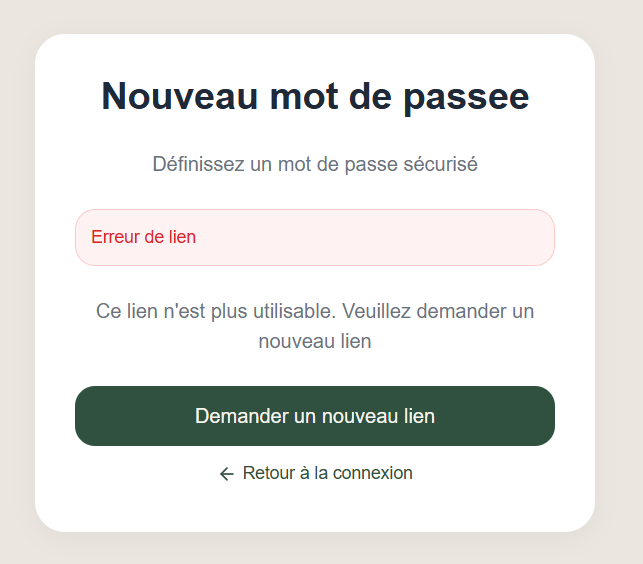
\includegraphics[width=\linewidth]{project/images/invalid-link.png}
        \captionof{figure}{Interface de réinitialisation : lien invalide}
        \label{cap:Interface de réinitialisation: lien invalide}
    \end{minipage}

\end{center}

\vspace{0.5cm}
\noindent \textbf{Interface de création du nouvelle mot de passe:}

\noindent Si le lien est valide, l'utilisateur accède au formulaire de la Figure \ref{cap:reset_form}. Cette interface sécurisée permet de saisir et de confirmer le nouveau mot de passe.
Le système applique également des règles de validation afin de garantir la robustesse du mot de passe. Ainsi, si le mot de passe saisi ne respecte pas les contraintes définies, un message d’erreur s’affiche à l’écran, comme illustré dans la figure \ref{cap:reset_invalid}, invitant l’utilisateur à corriger sa saisie.

\noindent Enfin, après la validation du nouveau mot de passe, un message de succès s'affiche dans la figure \ref{cap:reset_success} et le système redirige automatiquement l'utilisateur vers la page de connexion pour s'authentifier.


\begin{center}
    \centering
    
    % الصف الأول (زوز صور)
    \begin{minipage}{0.45\textwidth}
        \centering
        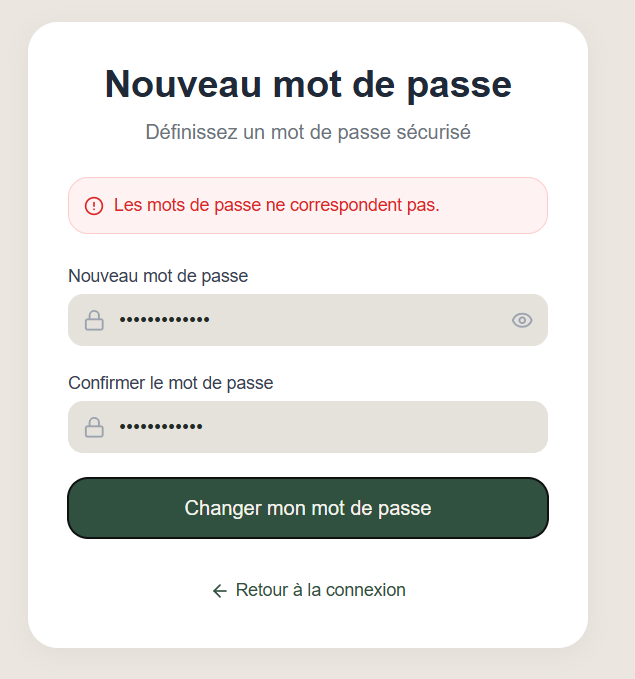
\includegraphics[width=1\linewidth]{project/images/reset-empty.png}
        \captionof{figure}{Interface de réinitialisation : changer le mot de passe}
        \label{cap:reset_form}
    \end{minipage}
    \hfill
    \begin{minipage}{0.45\textwidth}
        \centering
        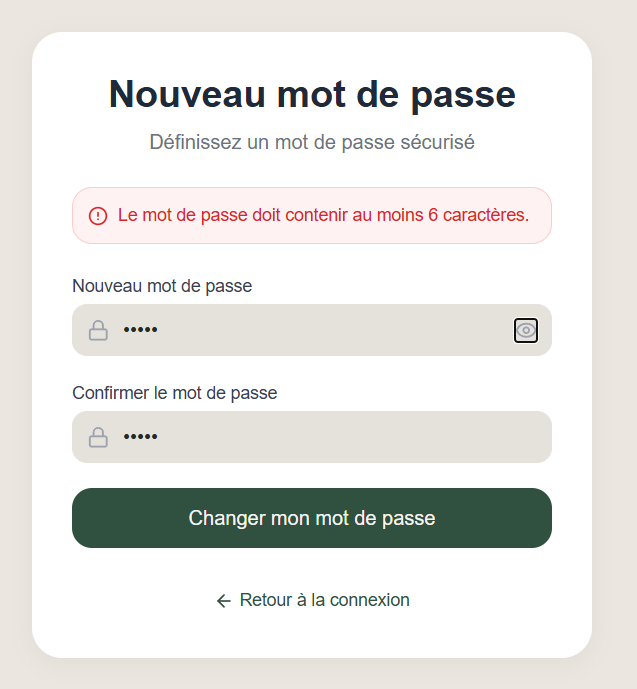
\includegraphics[width=1\linewidth]{project/images/ress-invalide.png}
        \captionof{figure}{Interface de réinitialisation : mot de passe invalide}
        \label{cap:reset_invalid}
    \end{minipage}
    
    \vspace{0.5cm} % espace بين الصفوف
    
    % الصف الثاني (صورة وحدة في الوسط)
    \begin{minipage}{0.7\textwidth}
        \centering
        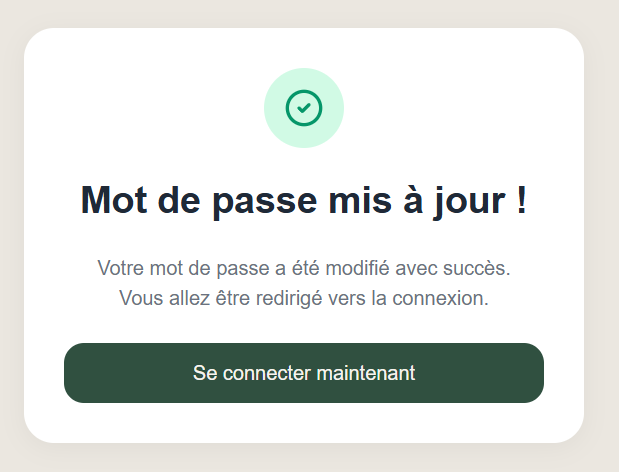
\includegraphics[width=0.8\linewidth]{project/images/ress-success.png}
        \captionof{figure}{Interface de réinitialisation : mot de passe réinitialisé avec succès}
        \label{cap:reset_success}
    \end{minipage}
\end{center}


\section{Sprint 2: Gestion des utilisateurs}
\label{sec:sprint2-gestion-utilisateurs}
Le sprint 2 est consacré au développement du module de gestion des utilisateurs, une fonctionnalité essentielle de notre système.
Ce module permet aux administrateurs de gérer efficacement l’ensemble des utilisateurs de la plateforme, notamment à travers la consultation, la validation (acceptation ou refus), la suppression ainsi que la mise à jour de leurs informations.
L’objectif de ce sprint est de mettre en place une interface intuitive, ergonomique et sécurisée, offrant une gestion complète et centralisée des comptes utilisateurs, afin de répondre aux besoins d’administration du système.
\subsection{Le backlog du sprint 2}
Le backlog du Sprint 2, consigné dans le Tableau \ref{tab:backlog_sprint2}, recense les fonctionnalités de gestion des utilisateurs à développer. Il fournit ainsi un cadre structuré pour l'ordonnancement et le suivi des tâches de cette itération.
\nopagebreak

\begin{table}[H]
\caption{Backlog - Gestion des utilisateurs}
\label{tab:backlog_sprint2}
\centering
\small
\setlength{\tabcolsep}{3pt}
\renewcommand{\arraystretch}{0.85}

\begin{tabular}{|c|>{\centering\arraybackslash}p{2.8cm}|p{9cm}|c|}
\hline
\textbf{ID} & \textbf{Fonctionnalité} & \textbf{User Stories} & \textbf{Priorité} \\
\hline
\multirow{6}{*}{2} & \multirow{6}{=}{\small Gestion des utilisateurs} 
& En tant qu'administrateur, je veux consulter la liste des utilisateurs afin de gérer les comptes & M \\ \cline{3-4}
& & En tant qu'administrateur, je veux modifier les informations d'un utilisateur afin de maintenir les données à jour & M \\ \cline{3-4}
& & En tant qu'administrateur, je veux supprimer un utilisateur afin de retirer les comptes inutiles & M \\ \cline{3-4}
& & En tant qu'administrateur, je veux approuver ou refuser les demandes afin de contrôler l'accès & M \\ \cline{3-4}
& & En tant qu'administrateur, je veux ajouter un nouvel utilisateur afin de créer des comptes & S \\ \cline{3-4}
& & En tant qu'administrateur, je veux activer ou désactiver un utilisateur afin de gérer son statut & S \\
\hline
\end{tabular}

\end{table}

\subsection{Analyse}
L'analyse du module de gestion des utilisateurs nous a permis d'identifier les besoins fonctionnels et de définir précisément les interactions attendues entre l'administrateur et le système
\vspace{0.3cm}

\noindent\textbf{Amélioration du cas d’utilisation « gestion des utilisateurs »:}
 
\noindent Le cas d'utilisation « gestion des utilisateurs » permet à l’administrateur d'effectuer toutes les opérations nécessaires à la gestion efficace des comptes utilisateurs au sein du système.
\vspace{0.3cm}

\noindent La figure \ref{fig:usecase_gestion_utilisateurs} présente le diagramme de cas d'utilisation illustrant les différents scénarios de gestion des utilisateurs, et détaillant les différentes actions que l’administrateur peut réaliser.
 \begin{figure}[H]
    \centering
    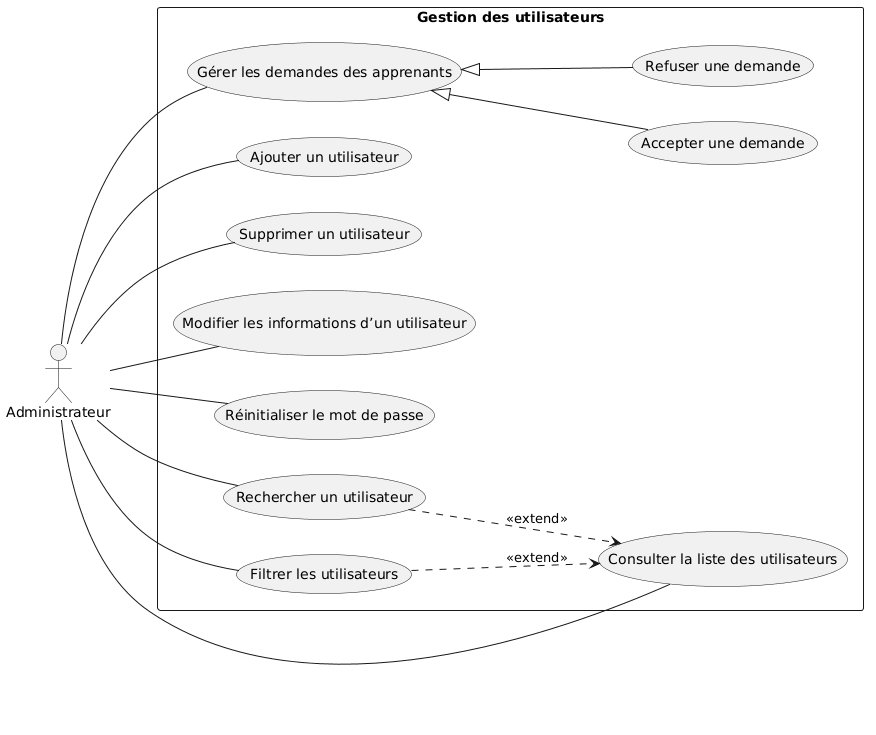
\includegraphics[width=1\textwidth]{project/images/new DG.png}
    \caption{Diagramme de cas d'utilisation "gestion des utilisateurs"}
    \label{fig:usecase_gestion_utilisateurs}
\end{figure}

Le tableau \ref{tab:gestion_utilisateurs} présente la description textuelle du cas d'utilisation « gestion des utilisateurs ».
{\interlinepenalty=10000
\begin{longtable}{|l|p{12cm}|}
\caption{Cas d'utilisation -- Gestion des utilisateurs}
\label{tab:gestion_utilisateurs} \\
\hline
\textbf{Élément} & \textbf{Description} \\
\hline
\endfirsthead
\hline
\textbf{Élément} & \textbf{Description} \\
\hline
\endhead

Cas d'utilisation & Gestion des utilisateurs \\
\hline
Acteur & Administrateur \\
\hline

Préconditions &
L'administrateur est connecté au système (authentifié). \\
& Le système est fonctionnel. \\
& La base de données est accessible. \\
\hline

Scénario de base &
\textbf{Scénario 1 : Consulter la liste des utilisateurs} \\
&- L'administrateur accède à l'interface Gestion des Utilisateurs. \\
&- Le système vérifie la validité du token. \\
&- Le système contrôle que l'utilisateur possède bien le rôle ADMIN. \\
&- Le système renvoie la liste complète des utilisateurs. \\
\\
& \textbf{Scénario 2 : Filtrage des utilisateurs} \\
&- L'administrateur applique un filtre (exemple : Rôle : directeur). \\
&- Le système met à jour dynamiquement le tableau sans rechargement de la page. \\
&- Le système affiche la liste filtrée. \\
\\
& \textbf{Scénario 3 : Rechercher un utilisateur} \\
&- L'administrateur saisit un nom ou un email dans le champ de recherche. \\
&- Le système effectue une recherche en temps réel et met à jour la liste des utilisateurs. \\
&- Le système affiche les résultats correspondants. \\
\\
& \textbf{Scénario 4 : Modifier les informations d'un utilisateur} \\
&- L'administrateur sélectionne un utilisateur dans la liste. \\
&- Le système affiche les détails de l'utilisateur. \\
&- L'administrateur modifie les informations souhaitées. \\
&- Le système met à jour les données de l'utilisateur. \\
\\
& \textbf{Scénario 5 : Ajouter un utilisateur} \\
&- L'administrateur clique sur « Nouvel utilisateur ». \\
&- Le système affiche le formulaire d'ajout. \\
&- L'administrateur renseigne les informations nécessaires (nom, prénom, email, rôle). \\
&- L'administrateur valide la création. \\
&- Le système vérifie la validité des données et l'unicité de l'email. \\
&- Le système hache le mot de passe (bcrypt). \\
&- Le système enregistre le nouvel utilisateur. \\
\\
& \textbf{Scénario 6 : Supprimer un utilisateur} \\
&- L'administrateur sélectionne un utilisateur dans la liste. \\
&- Le système affiche une confirmation de suppression. \\
&- L'administrateur confirme la suppression. \\
\hline
&- Le système supprime l'utilisateur de la base de données. \\
\\
& \textbf{Scénario 7 : Réinitialiser le mot de passe} \\
&- L'administrateur sélectionne un utilisateur. \\
&- Le système envoie un email de réinitialisation à l'utilisateur. \\
&- L'utilisateur saisit un nouveau mot de passe. \\
&- Le système vérifie la validité du mot de passe. \\
&- Le système hache le nouveau mot de passe (bcrypt). \\
&- Le système met à jour les données de l'utilisateur. \\
&- Le système confirme la réussite de l'opération. \\
\\
& \textbf{Scénario 8 : Gérer les demandes des apprenants} \\
&- L'administrateur accède à la section « Apprenants ». \\
&- Le système affiche la liste des apprenants en attente de validation. \\
&- L'administrateur accède à la liste des demandes d'inscription. \\
&- L'administrateur traite la demande (acceptation ou refus). \\
&- Le système met à jour le statut de la demande. \\
&- En cas d'acceptation, le système crée un compte utilisateur pour l'apprenant. \\
&- Le système envoie une notification à l'apprenant. \\
&- En cas de refus, le système archive la demande. \\
\hline

Scénarios alternatifs &
\textbf{Cas 1 -- Échec d'authentification :} Le système détecte un token invalide ou expiré et refuse l'accès. \\
& \textbf{Cas 2 -- Données invalides lors de l'ajout ou modification :} Le système détecte des informations incorrectes ou incomplètes et affiche un message d'erreur. \\
& \textbf{Cas 3 -- Échec d'envoi de l'email de réinitialisation :} Le système ne parvient pas à envoyer l'email et informe l'administrateur de l'échec. \\
\hline

Post-conditions &
\textbf{Scénarios 1, 2 et 3 :} La liste des utilisateurs (complète, filtrée ou recherchée) est affichée à l'administrateur. \\
& \textbf{Scénario 4 :} Les informations de l'utilisateur sélectionné sont mises à jour dans le système. \\
& \textbf{Scénario 5 :} Un nouveau compte utilisateur est créé, le mot de passe est haché et les données sont enregistrées dans la base de données. \\
& \textbf{Scénario 6 :} L'utilisateur sélectionné est définitivement supprimé de la base de données. \\
& \textbf{Scénario 7 :} Un email de réinitialisation est envoyé et le nouveau mot de passe haché est mis à jour dans le système. \\
& \textbf{Scénario 8 :} Le statut de la demande est mis à jour, un compte est créé en cas d'acceptation et une notification est envoyée à l'apprenant. \\
\hline
\end{longtable}
}

\vspace{0.2cm}

\subsection{Conception}
La section Conception présente la modélisation dynamique des principaux scénarios fonctionnels du module de gestion des utilisateurs. Les diagrammes de séquence ci-dessous illustrent, de manière chronologique et détaillée, les interactions entre les différents acteurs du système (Administrateur, Frontend, Backend, Base de données et Serveur Email), en couvrant les flux nominaux ainsi que les cas alternatifs et d'erreur.

\vspace{0.3cm}

\noindent \textbf{Diagramme de séquence : Ajouter un utiliateur}

\noindent Le diagramme de séquence de la Figure \ref{cap:Diagramme de séquence <<Ajouter un utilisateur>>} illustre le processus d'ajout d'un nouvel utilisateur par l'administrateur, depuis la saisie du formulaire jusqu'à l'enregistrement en base de données.
\begin{figure}[H]
  \centering
   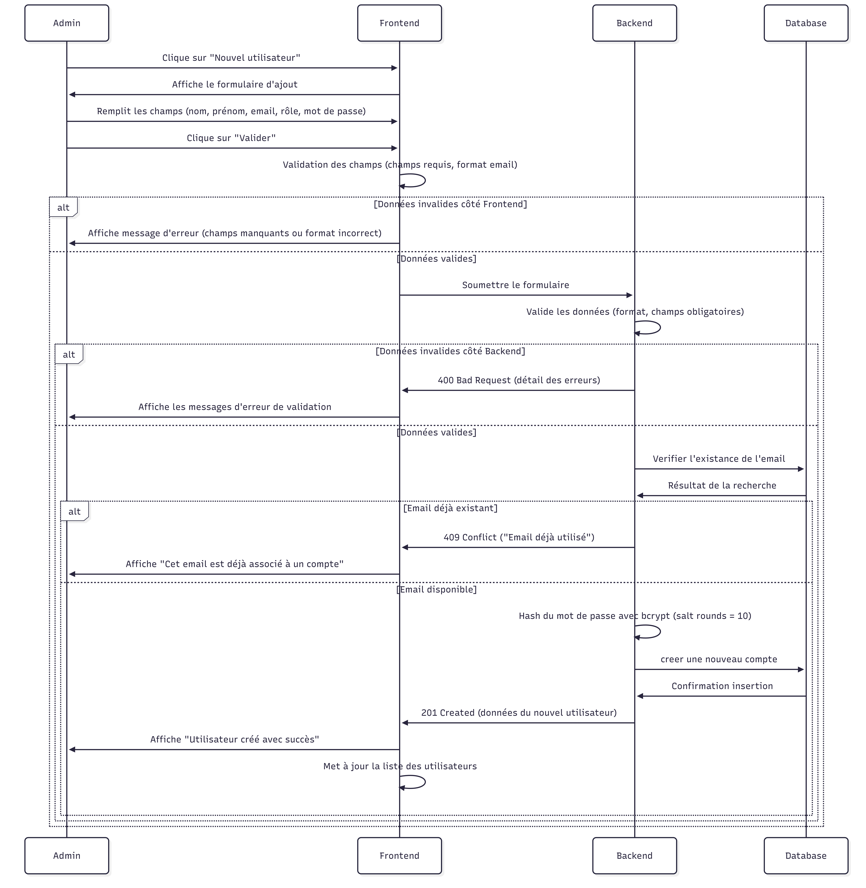
\includegraphics[scale=0.7]{project/images/ajouter-user.png}
  \caption{Diagramme de séquence <<Ajouter un utilisateur>> }
  \label{cap:Diagramme de séquence <<Ajouter un utilisateur>>}
\end{figure}
\vspace*{\fill} % espace vertical sous
\newpage
\noindent\textbf{Diagramme de séquence : Réinitialisation du mot de passe}

\noindent La Figure \ref{cap:Diagramme de séquence <<Réinitialisation du mot de passe>>} présente le diagramme de séquence relatif à la réinitialisation du mot de passe d'un utilisateur, initié par l'administrateur.
\begin{figure}[H]
  \centering
    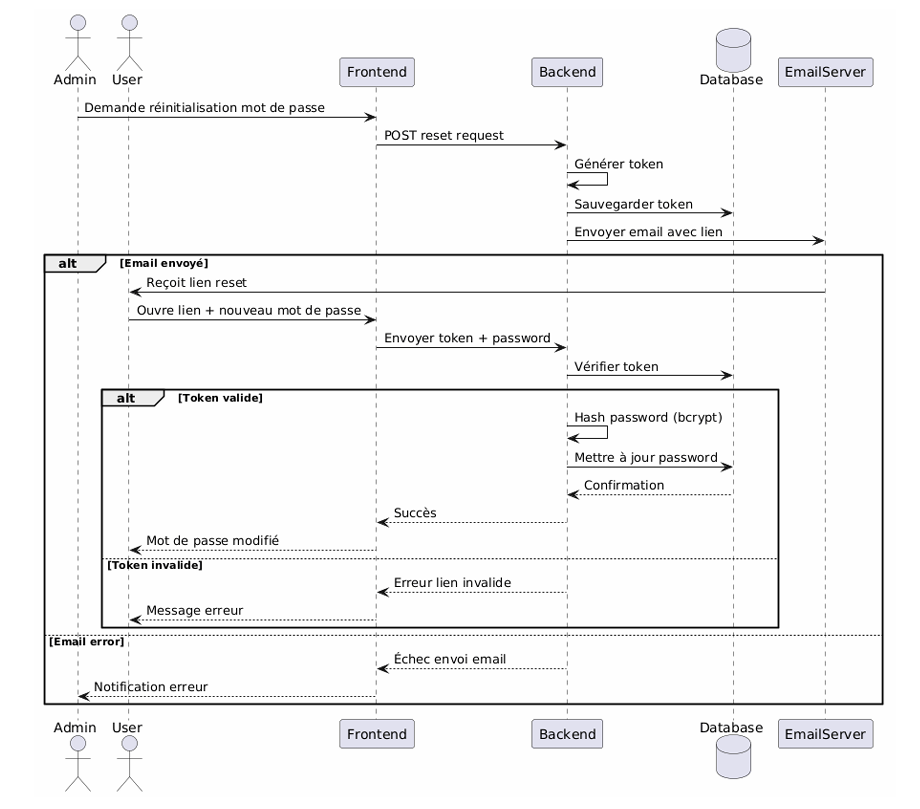
\includegraphics[scale=0.7]{project/images/admin-réinitialise.png}
  \caption{Diagramme de séquence <<Réinitialisation du mot de passe>> }
  \label{cap:Diagramme de séquence <<Réinitialisation du mot de passe>>}
\end{figure}
\vspace*{\fill} 

\newpage

\noindent \textbf{Diagramme de séquence : Gestion des demandes des apprenants}


\noindent Le diagramme de séquence de la Figure \ref{cap:Diagramme de séquence <<Gestion des demandes des apprenants>>} décrit le flux de traitement des demandes d'inscription des apprenants par l'administrateur, en détaillant les deux chemins possibles: l'acceptation, qui declanche l'envoi d'une notification par email, et le refus, qui archive la demande et notifie l'apprenant.
\begin{figure}[H]
  \centering
    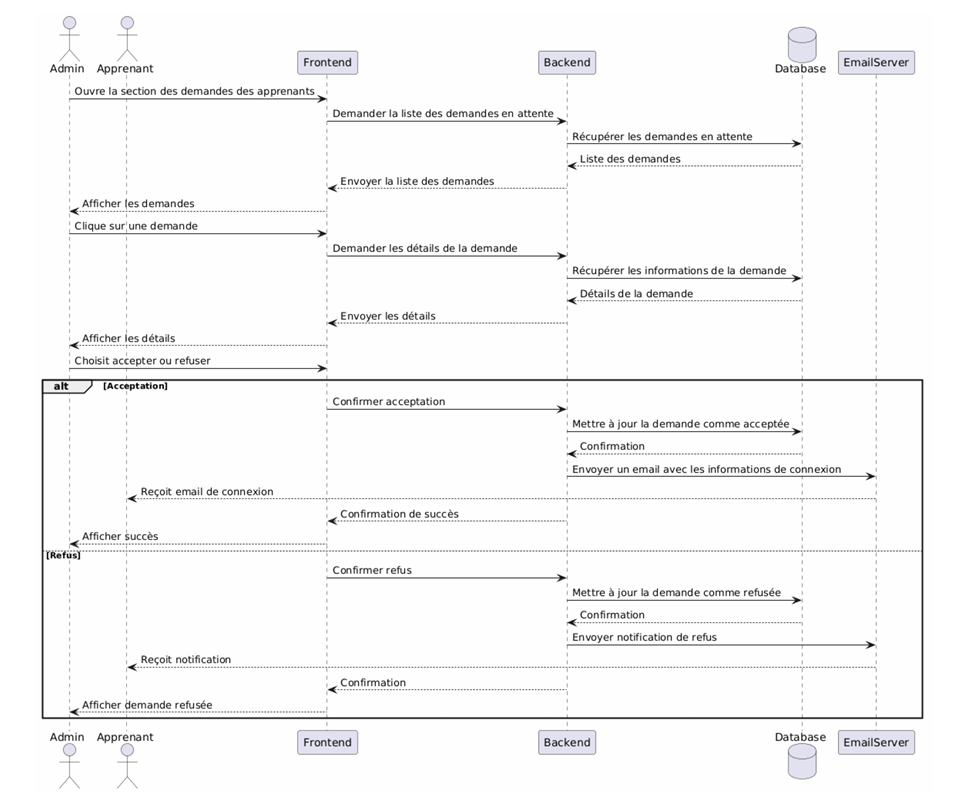
\includegraphics[scale=0.7]{project/images/accept-rejectsequence.png}
  \caption{Diagramme de séquence <<Gestion des demandes des apprenants>> }
  \label{cap:Diagramme de séquence <<Gestion des demandes des apprenants>>}
\end{figure}

\subsection{Réalisation}
Cette section présente les interfaces de gestion des utilisateurs, en mettant l’accent sur les différentes fonctionnalités implémentées et l’expérience utilisateur offerte par ces interfaces.

\vspace{0.3cm}
\noindent \textbf{Interface de gestion des utilisateurs :} 

\noindent La figure \ref{fig:capture_userstab} présente l'interface principale affichant la liste des utilisateurs sous forme de tableau structuré, avec barre de recherche et filtres par rôle.

\begin{figure}[H]  % [H] bech t7otha houni just
    \centering
    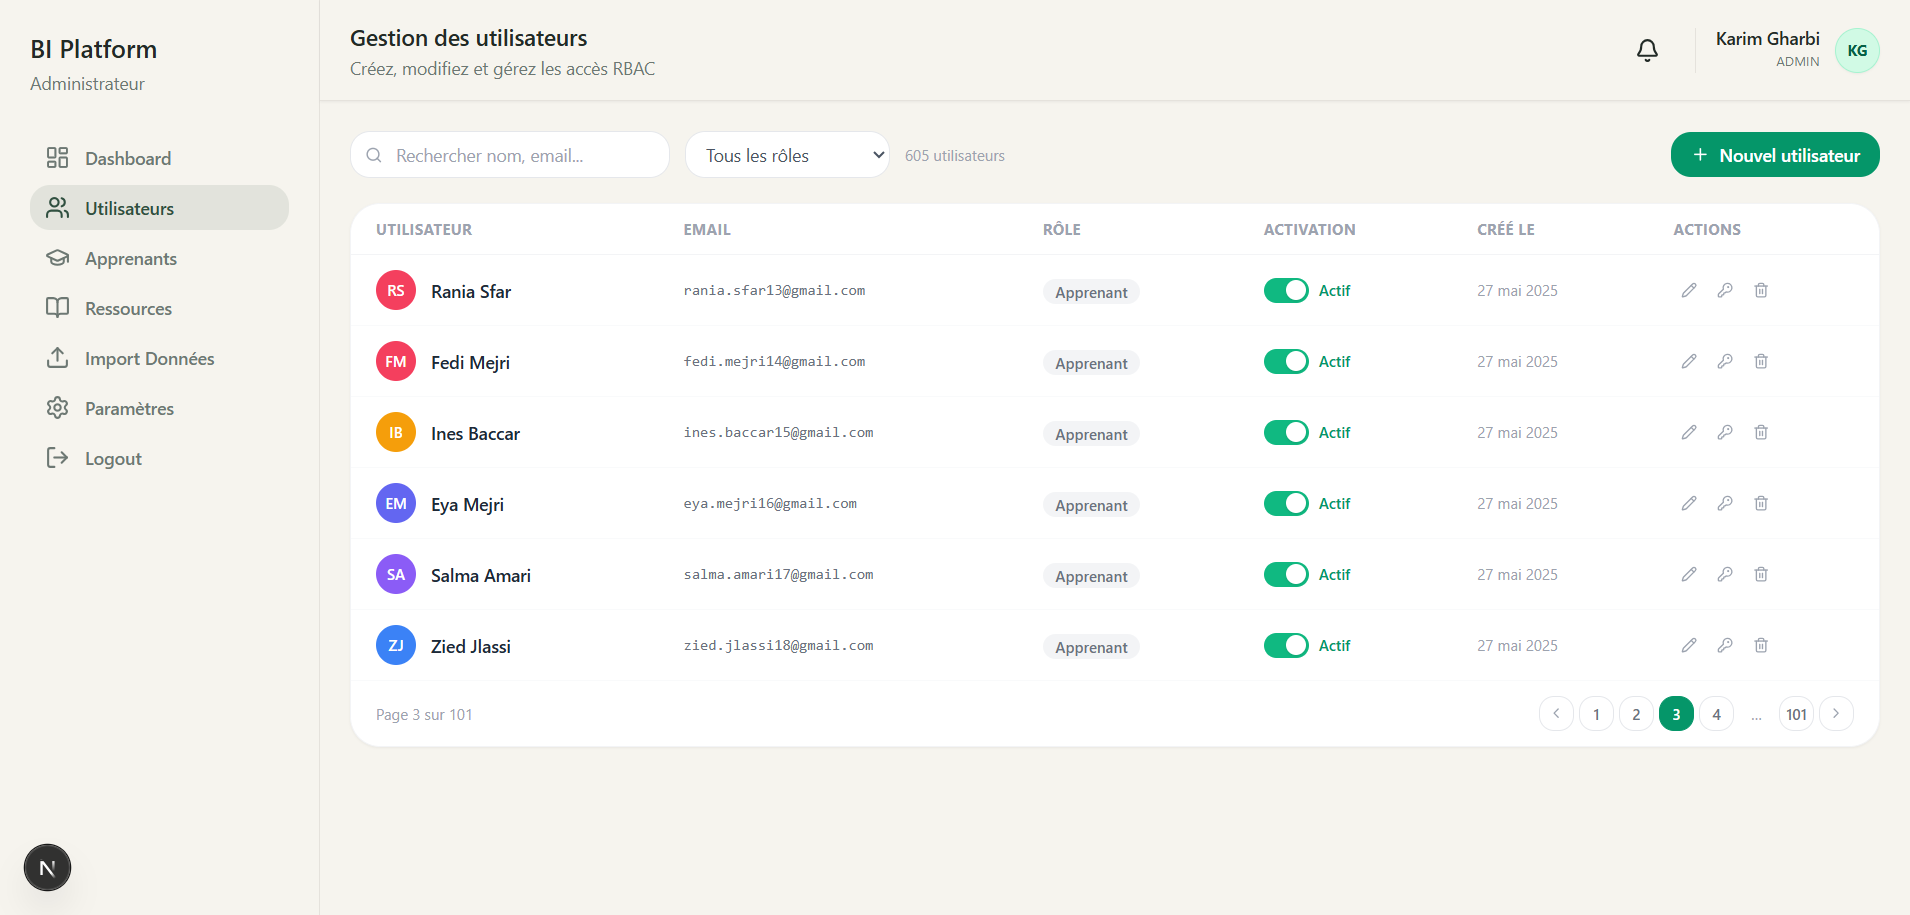
\includegraphics[width=0.8\textwidth]{project/images/localhost_3000_admin_users.png}
    \caption{Gestion des utilisateurs}
    \label{fig:capture_userstab}
\end{figure}

\noindent\textbf{Validation des comptes :} 

\noindent La figure \ref{fig:capture_learnersvalidated} illustre l'interface de traitement des demandes d'inscription, permettant à l'administrateur d'accepter ou de refuser les comptes en attente.

\begin{figure}[H]  % [H] bech t7otha houni just
    \centering
    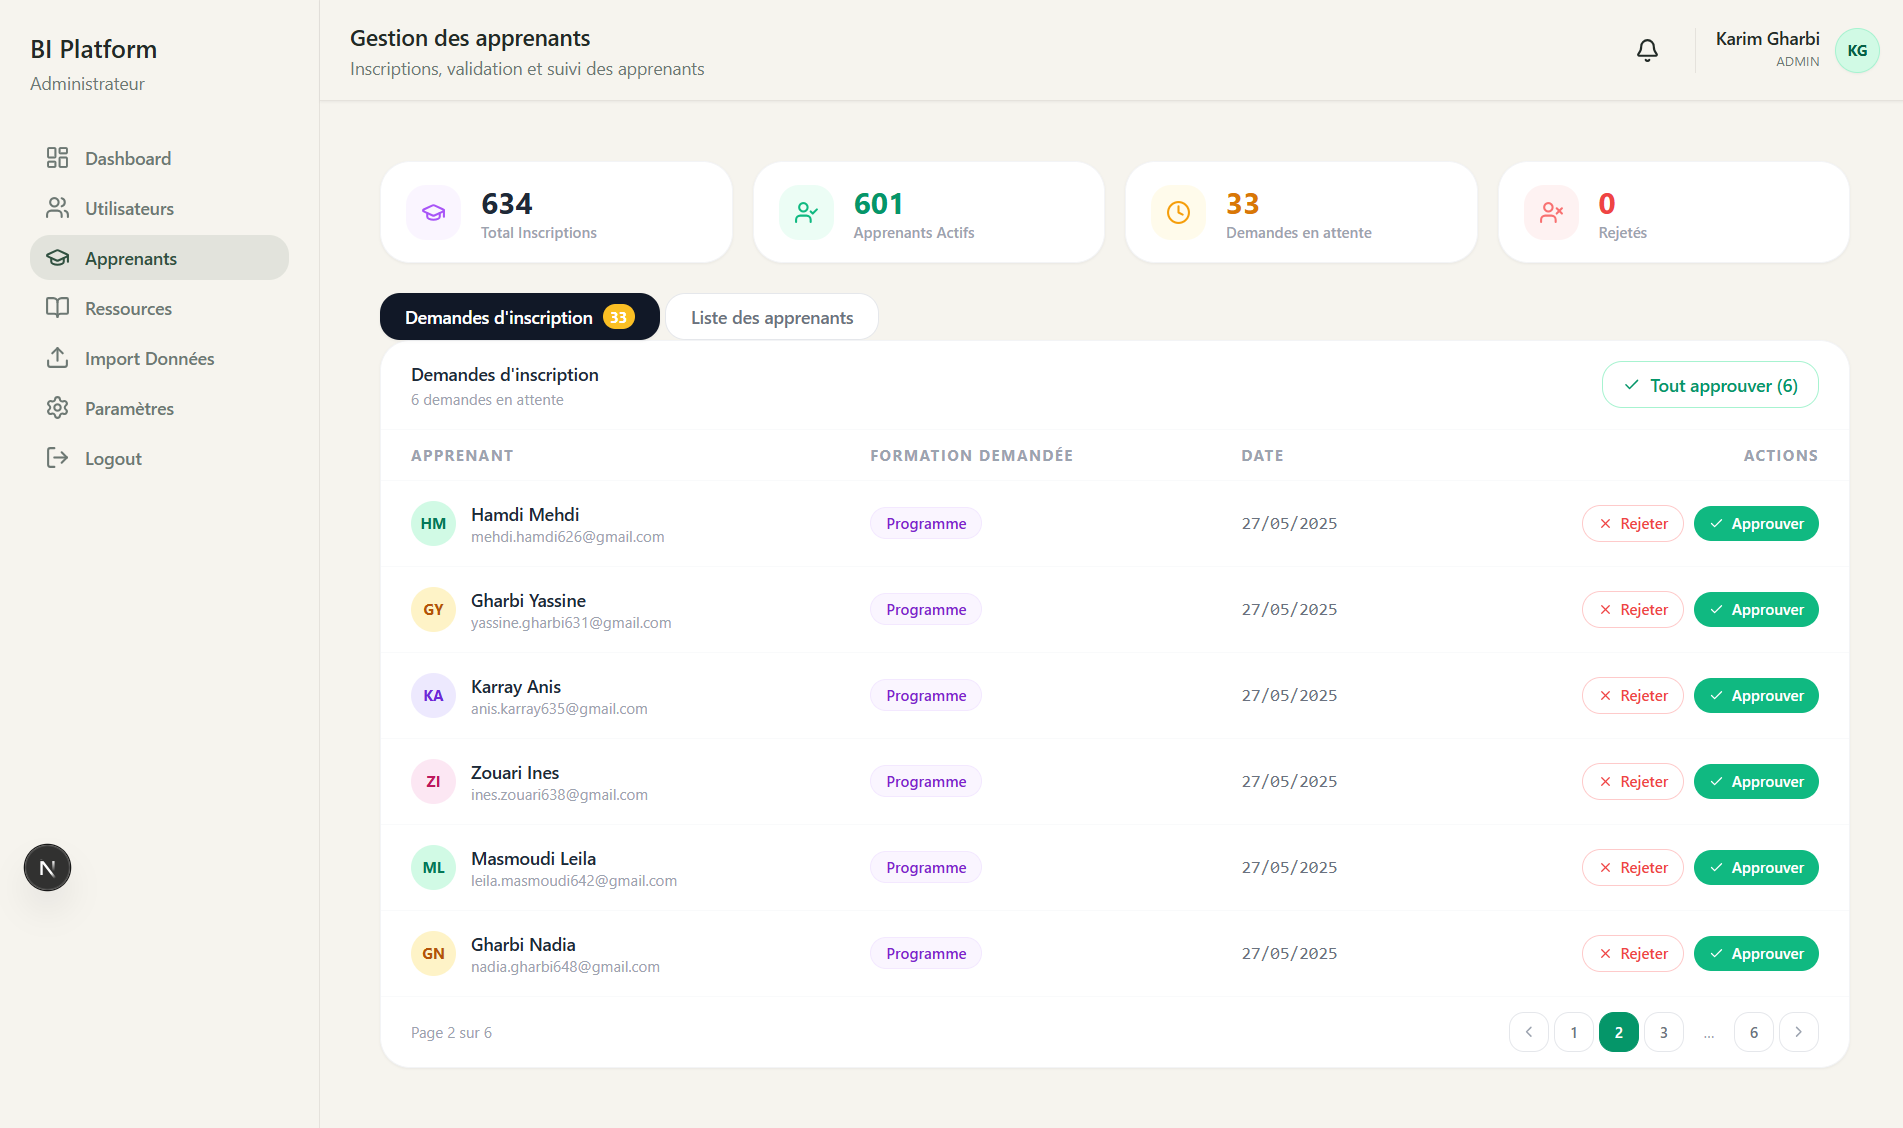
\includegraphics[width=0.9\textwidth]{project/images/localhost_3000_admin_learners.png}
    \caption{Gestion des demandes d'inscription des apprenants}
    \label{fig:capture_learnersvalidated}
\end{figure}

\noindent \textbf{Ajout d’un utilisateur :} 

\noindent La figure \ref{fig:capture_newuser} montre le modal d'ajout d'un nouvel utilisateur, comportant les champs nom, email, rôle et mot de passe.

\begin{figure}[H]  % [H] bech t7otha houni just
    \centering
    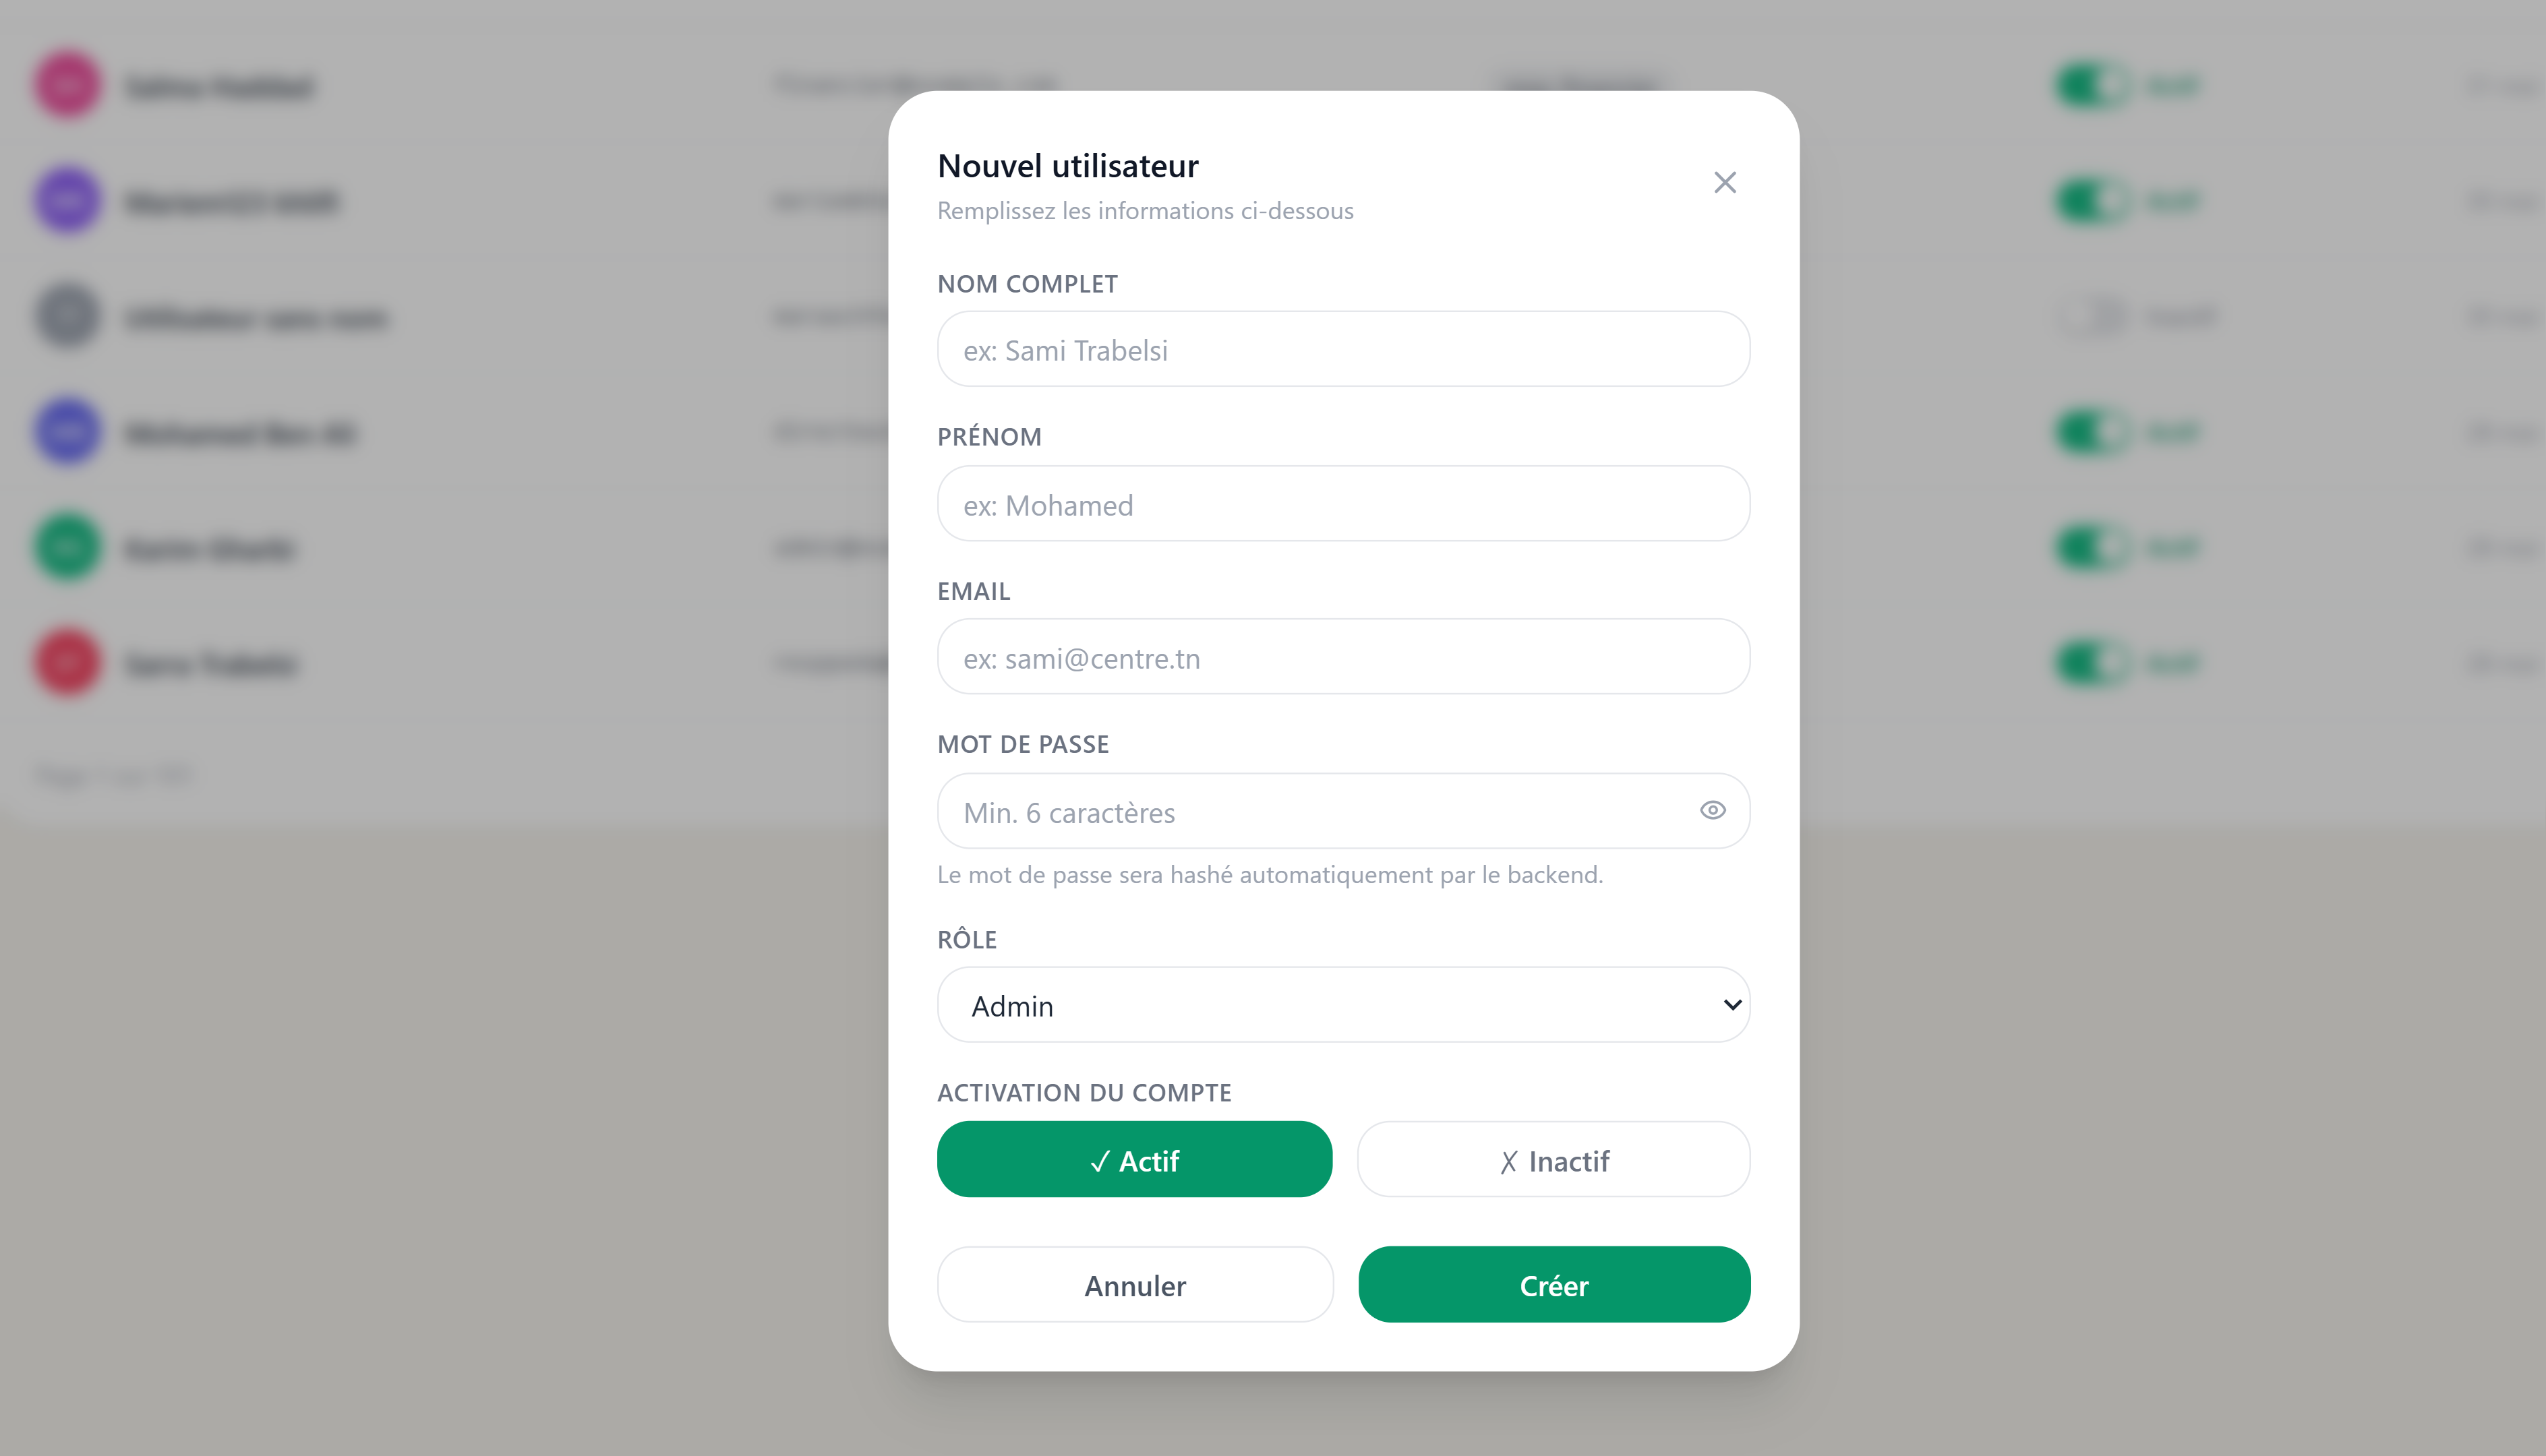
\includegraphics[width=0.8\textwidth]{project/images/newusers.png}
    \caption{Ajout d’un utilisateur}
    \label{fig:capture_newuser}
\end{figure}
\noindent \textbf{Modification des informations :} 

\noindent Les figures \ref{fig:reset-password} et \ref{fig:modifier-user} présentent respectivement la sélection d'un utilisateur et le modal de modification pré-rempli avec ses données actuelles.
\begin{figure}[H]
    \centering
    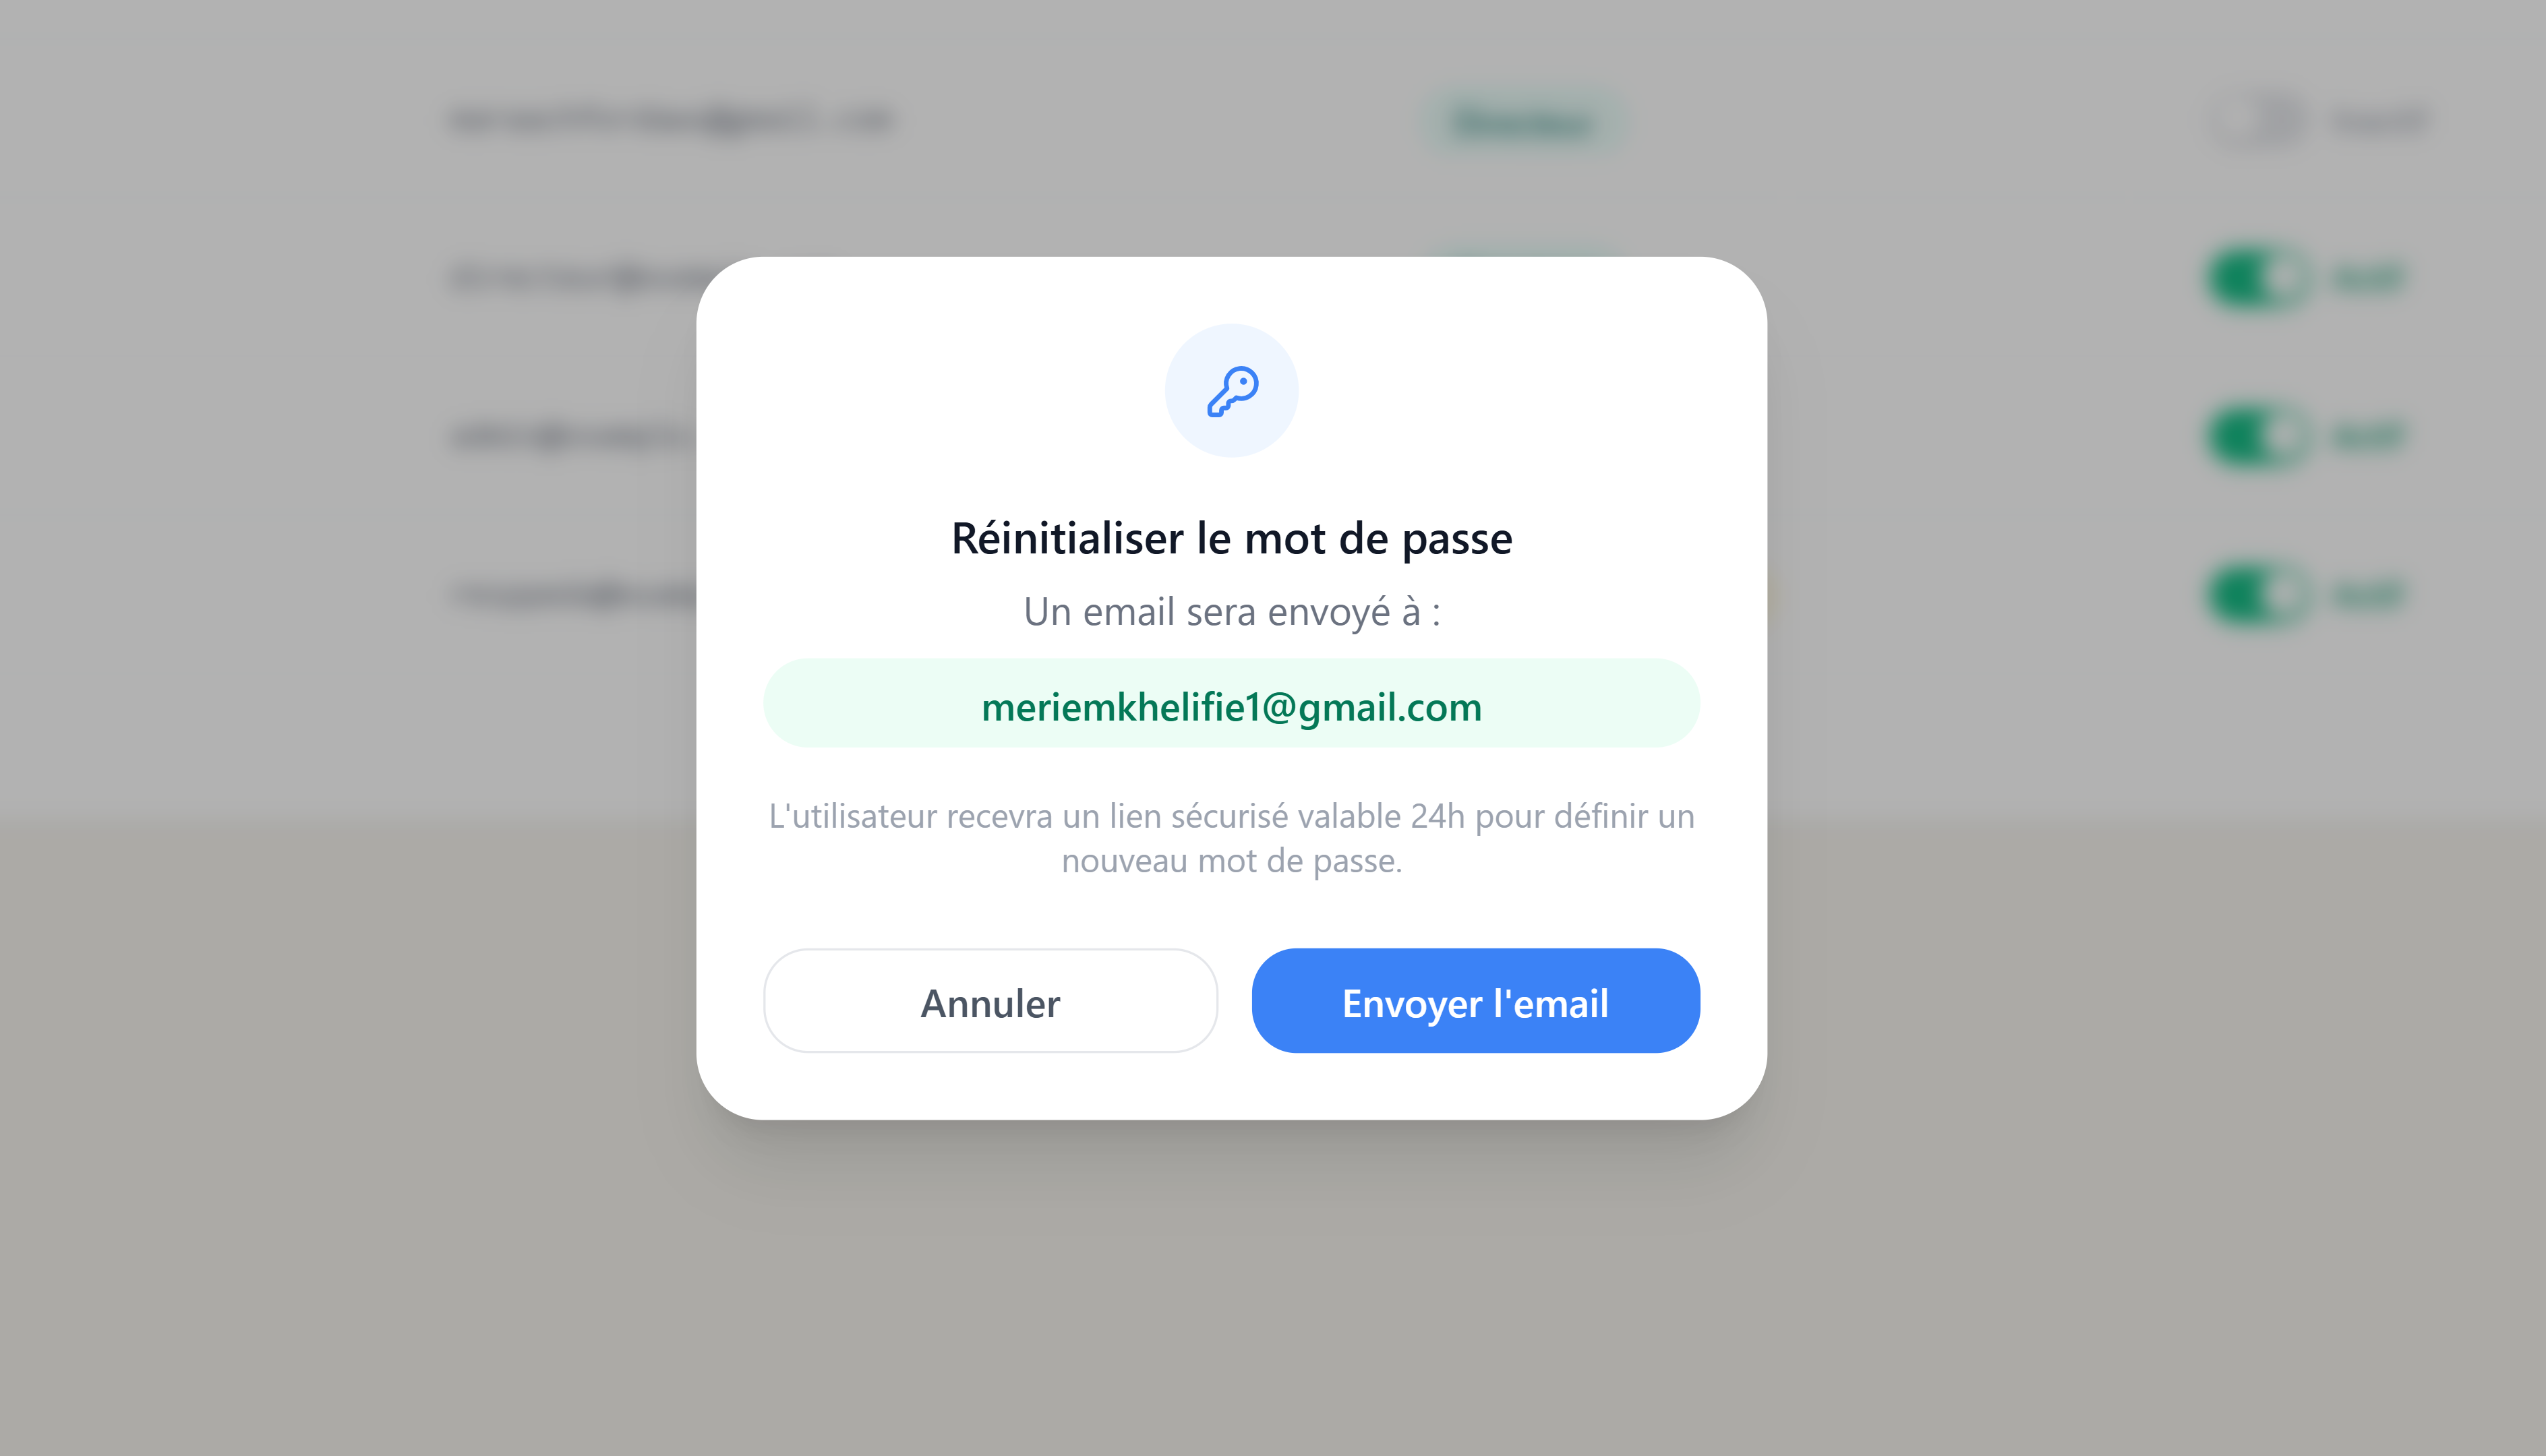
\includegraphics[width=0.6\textwidth]{project/images/resetPassword.png}
    \caption{Réinitialisation du mot de passe}
    \label{fig:reset-password}
\end{figure}

\begin{figure}[H]
    \centering
    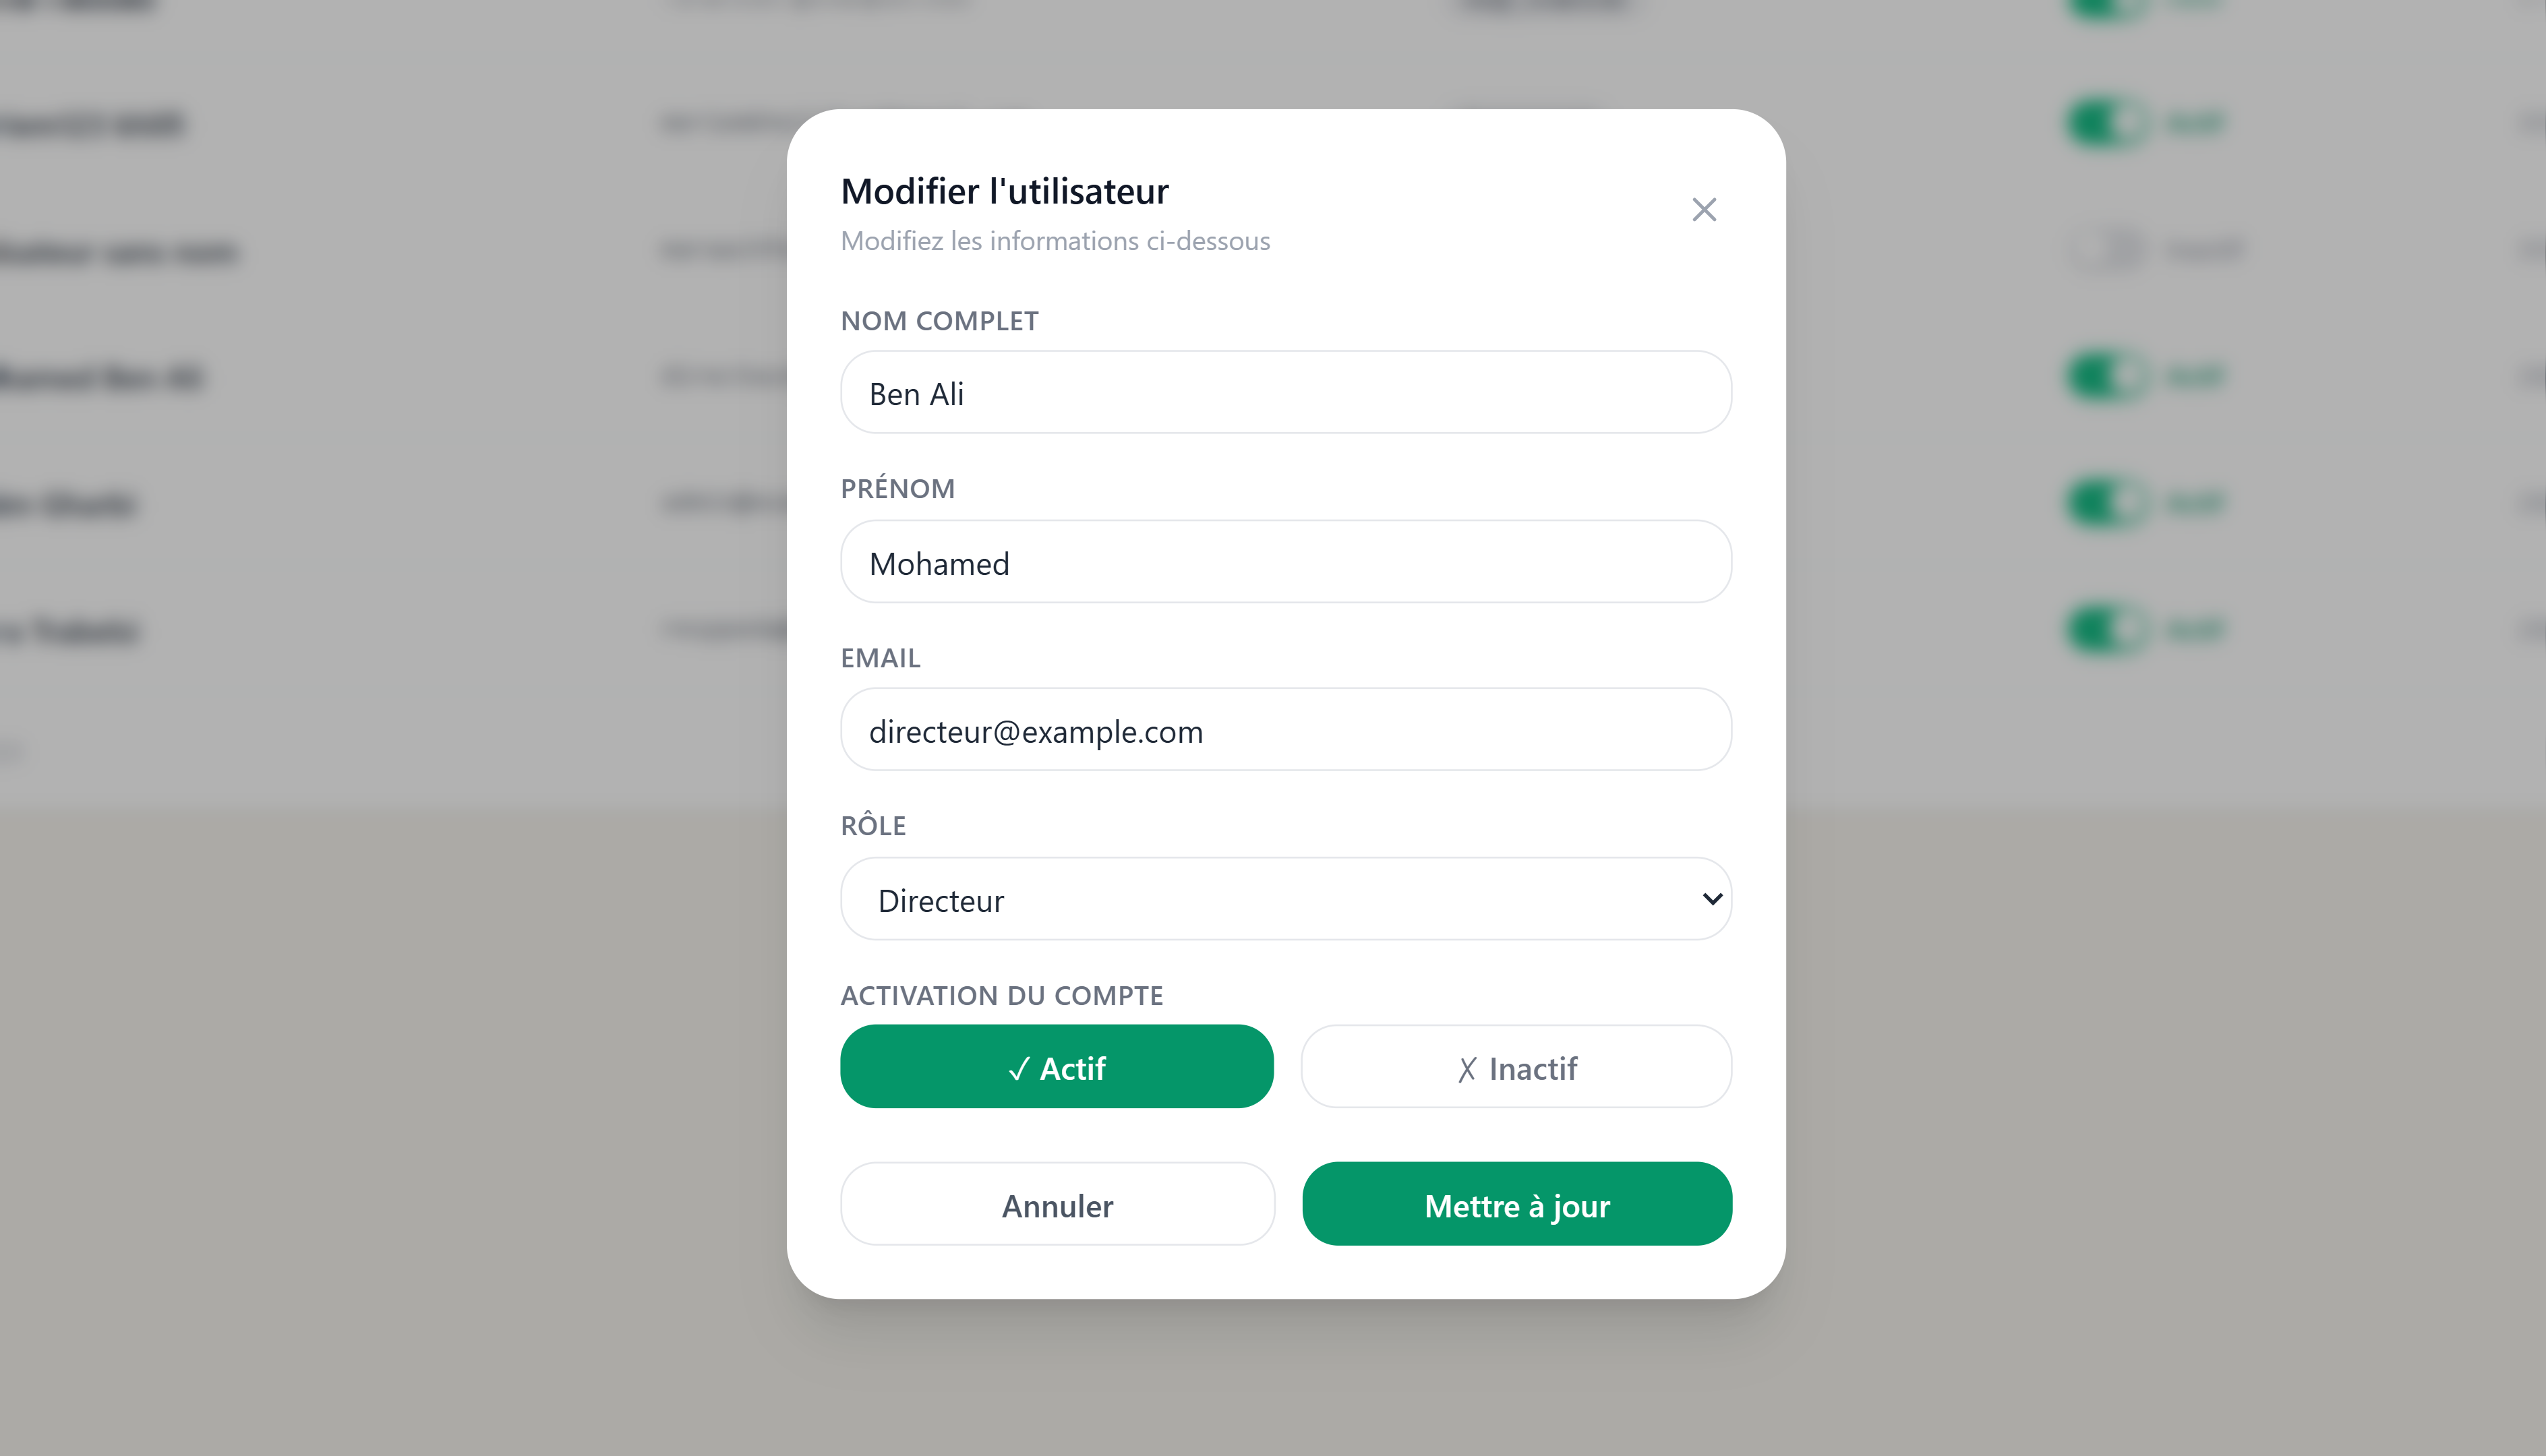
\includegraphics[width=0.6\textwidth]{project/images/ModfierUSERS.png}
    \caption{Modification d'un utilisateur}
    \label{fig:modifier-user}
\end{figure}

\textbf{Suppression d’un utilisateur :} 

\noindent La figure \ref{fig:capture_del} montre le modal de confirmation de suppression, invitant l'administrateur à confirmer ou annuler la suppression définitive du compte.

\begin{figure}[H]  % [H] bech t7otha houni just
    \centering
    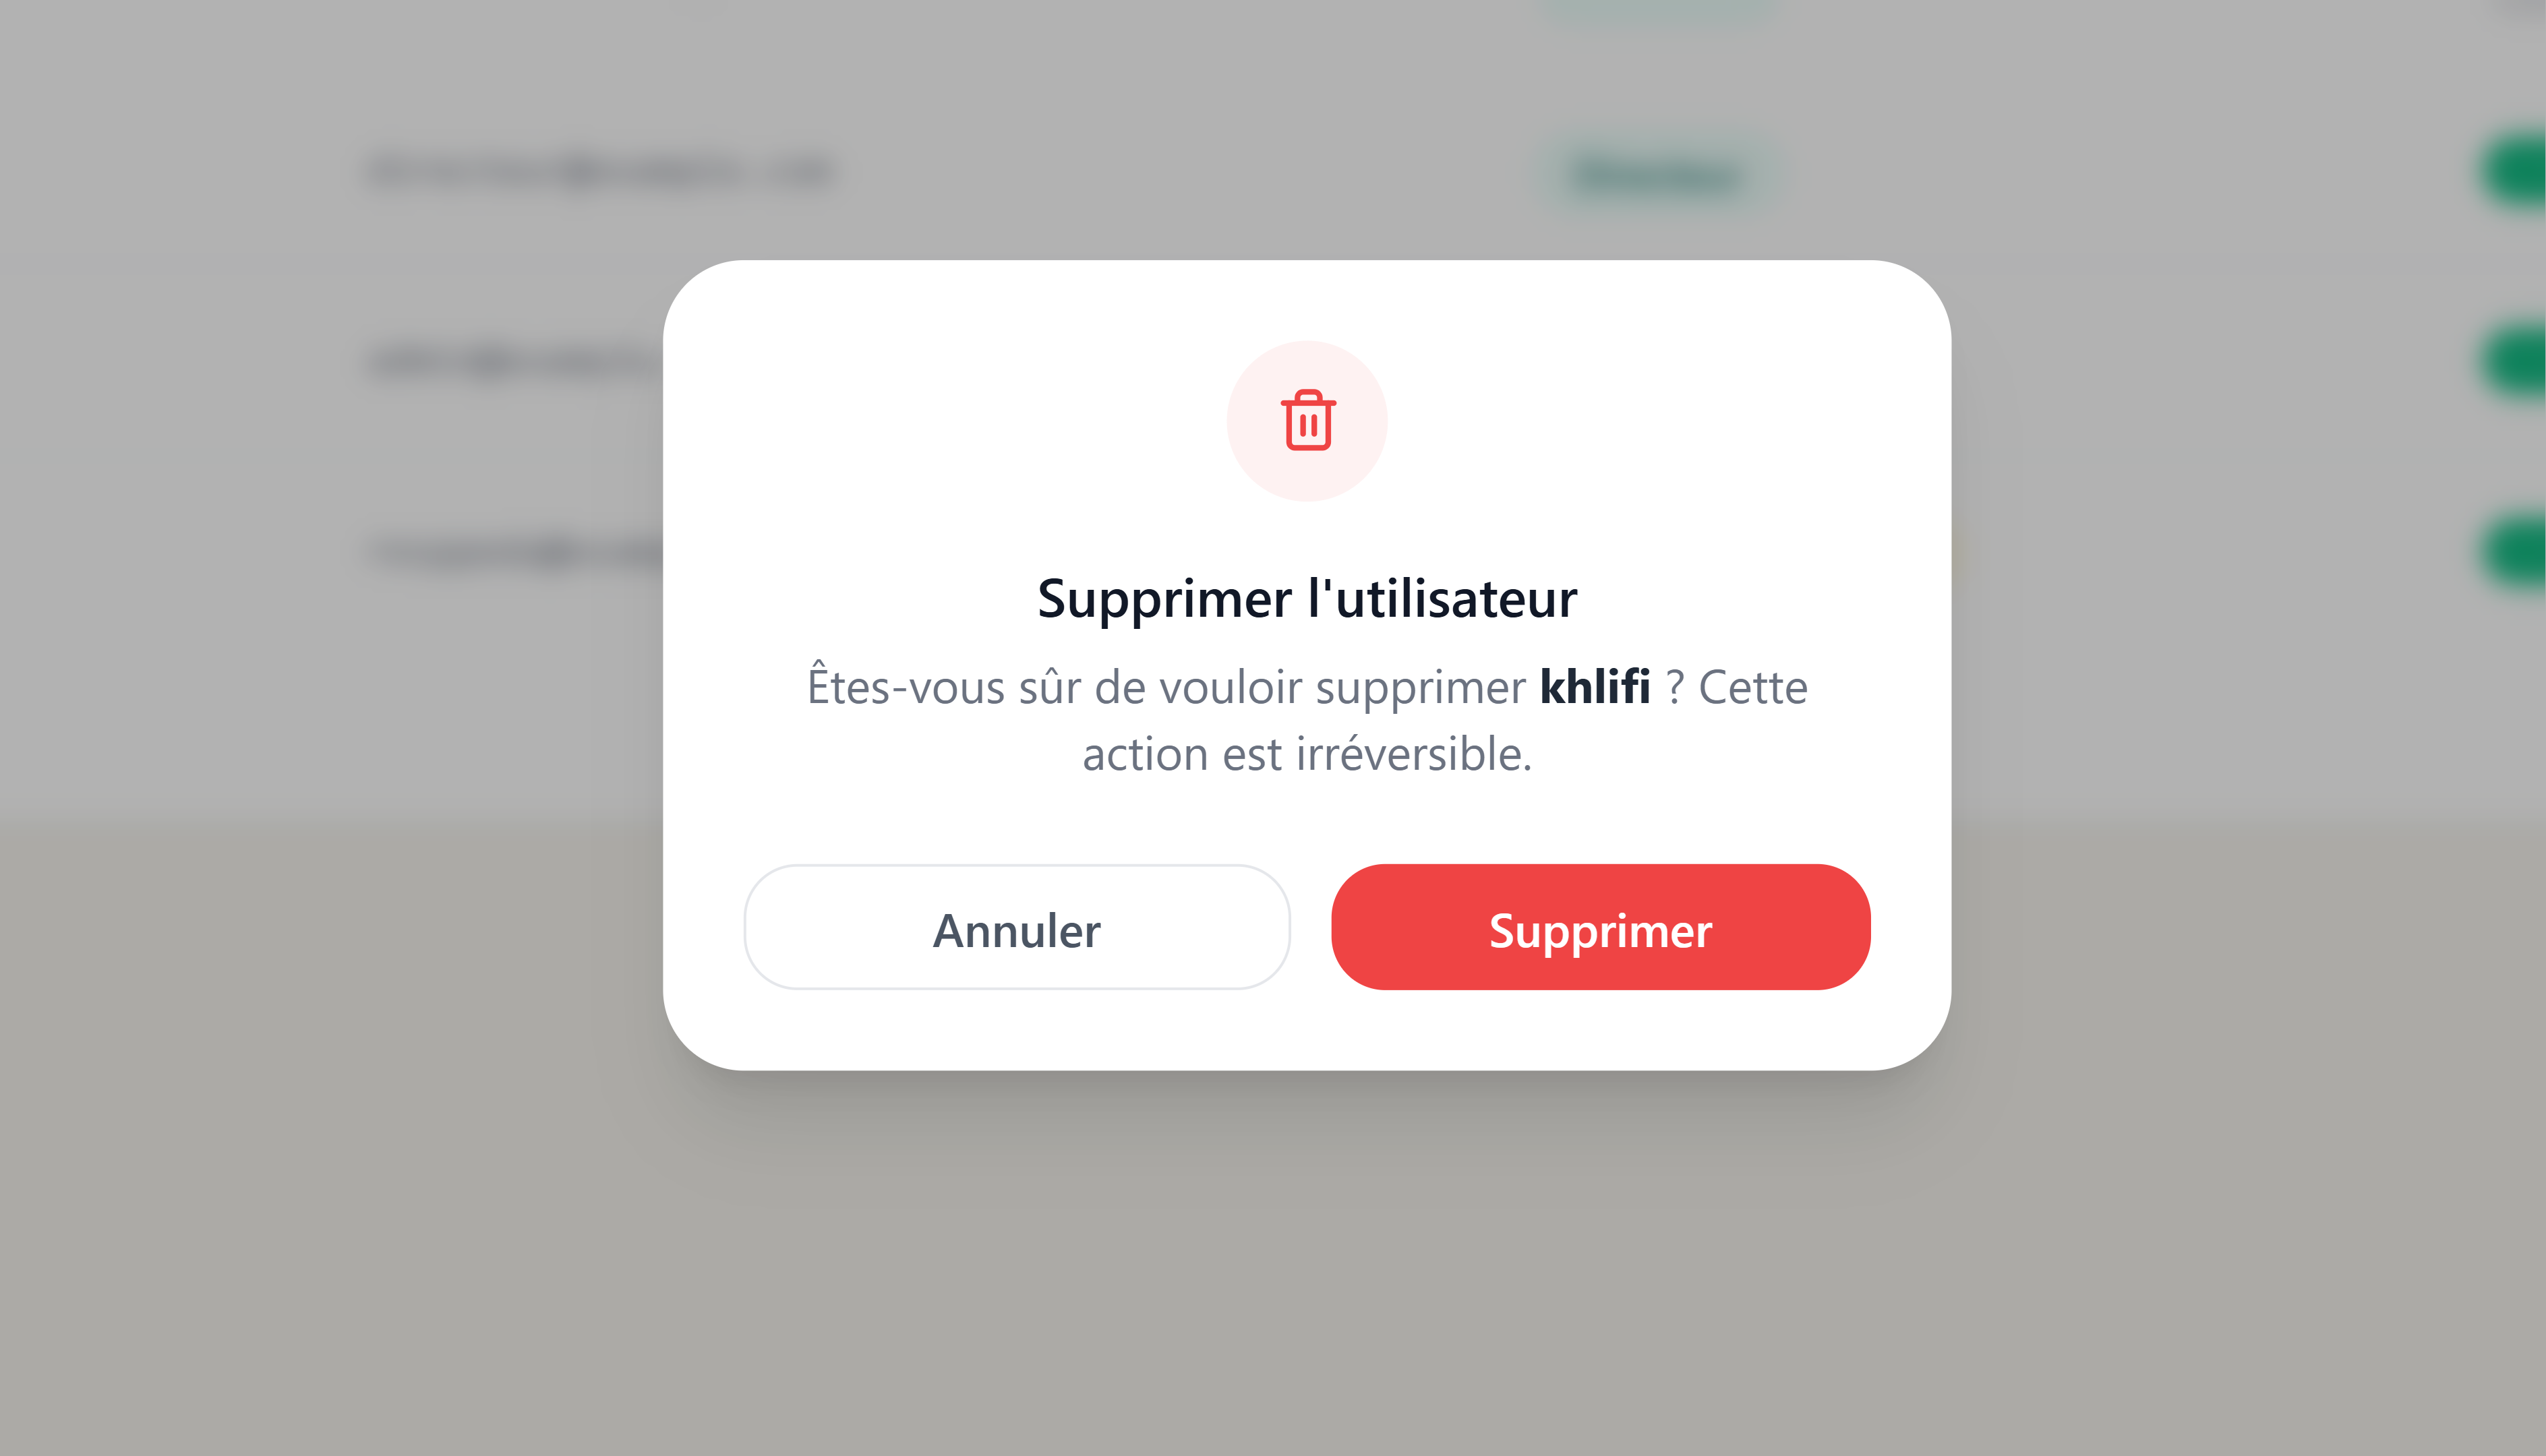
\includegraphics[width=0.8\textwidth]{project/images/deleteUsers.png}
    \caption{Suppression d'un utilisateur}
    \label{fig:capture_del}
\end{figure}

\section{Conclusion}
Ce chapitre a présenté la première release de la plateforme, organisée en deux sprints principaux. Le premier sprint a concerné la mise en place de l’authentification afin de sécuriser l’accès au système, tandis que le second a porté sur la gestion des utilisateurs et des rôles.

\noindent L’ensemble du développement a suivi une démarche structurée basée sur l’analyse, la conception et la réalisation. Cette première version constitue une base fonctionnelle importante pour la suite du projet.
\bibliographystyle{IEEEtran}
\bibliography{references}
\end{document}
